\documentclass[twoside]{book}

% Packages required by doxygen
\usepackage{fixltx2e}
\usepackage{calc}
\usepackage{doxygen}
\usepackage[export]{adjustbox} % also loads graphicx
\usepackage{graphicx}
\usepackage[utf8]{inputenc}
\usepackage{makeidx}
\usepackage{multicol}
\usepackage{multirow}
\PassOptionsToPackage{warn}{textcomp}
\usepackage{textcomp}
\usepackage[nointegrals]{wasysym}
\usepackage[table]{xcolor}

% Font selection
\usepackage[T1]{fontenc}
\usepackage[scaled=.90]{helvet}
\usepackage{courier}
\usepackage{amssymb}
\usepackage{sectsty}
\renewcommand{\familydefault}{\sfdefault}
\allsectionsfont{%
  \fontseries{bc}\selectfont%
  \color{darkgray}%
}
\renewcommand{\DoxyLabelFont}{%
  \fontseries{bc}\selectfont%
  \color{darkgray}%
}
\newcommand{\+}{\discretionary{\mbox{\scriptsize$\hookleftarrow$}}{}{}}

% Page & text layout
\usepackage{geometry}
\geometry{%
  a4paper,%
  top=2.5cm,%
  bottom=2.5cm,%
  left=2.5cm,%
  right=2.5cm%
}
\tolerance=750
\hfuzz=15pt
\hbadness=750
\setlength{\emergencystretch}{15pt}
\setlength{\parindent}{0cm}
\setlength{\parskip}{3ex plus 2ex minus 2ex}
\makeatletter
\renewcommand{\paragraph}{%
  \@startsection{paragraph}{4}{0ex}{-1.0ex}{1.0ex}{%
    \normalfont\normalsize\bfseries\SS@parafont%
  }%
}
\renewcommand{\subparagraph}{%
  \@startsection{subparagraph}{5}{0ex}{-1.0ex}{1.0ex}{%
    \normalfont\normalsize\bfseries\SS@subparafont%
  }%
}
\makeatother

% Headers & footers
\usepackage{fancyhdr}
\pagestyle{fancyplain}
\fancyhead[LE]{\fancyplain{}{\bfseries\thepage}}
\fancyhead[CE]{\fancyplain{}{}}
\fancyhead[RE]{\fancyplain{}{\bfseries\leftmark}}
\fancyhead[LO]{\fancyplain{}{\bfseries\rightmark}}
\fancyhead[CO]{\fancyplain{}{}}
\fancyhead[RO]{\fancyplain{}{\bfseries\thepage}}
\fancyfoot[LE]{\fancyplain{}{}}
\fancyfoot[CE]{\fancyplain{}{}}
\fancyfoot[RE]{\fancyplain{}{\bfseries\scriptsize Generated by Doxygen }}
\fancyfoot[LO]{\fancyplain{}{\bfseries\scriptsize Generated by Doxygen }}
\fancyfoot[CO]{\fancyplain{}{}}
\fancyfoot[RO]{\fancyplain{}{}}
\renewcommand{\footrulewidth}{0.4pt}
\renewcommand{\chaptermark}[1]{%
  \markboth{#1}{}%
}
\renewcommand{\sectionmark}[1]{%
  \markright{\thesection\ #1}%
}

% Indices & bibliography
\usepackage{natbib}
\usepackage[titles]{tocloft}
\setcounter{tocdepth}{3}
\setcounter{secnumdepth}{5}
\makeindex

% Hyperlinks (required, but should be loaded last)
\usepackage{ifpdf}
\ifpdf
  \usepackage[pdftex,pagebackref=true]{hyperref}
\else
  \usepackage[ps2pdf,pagebackref=true]{hyperref}
\fi
\hypersetup{%
  colorlinks=true,%
  linkcolor=blue,%
  citecolor=blue,%
  unicode%
}

% Custom commands
\newcommand{\clearemptydoublepage}{%
  \newpage{\pagestyle{empty}\cleardoublepage}%
}

\usepackage{caption}
\captionsetup{labelsep=space,justification=centering,font={bf},singlelinecheck=off,skip=4pt,position=top}

%===== C O N T E N T S =====

\begin{document}

% Titlepage & ToC
\hypersetup{pageanchor=false,
             bookmarksnumbered=true,
             pdfencoding=unicode
            }
\pagenumbering{alph}
\begin{titlepage}
\vspace*{7cm}
\begin{center}%
{\Large Tiny protocol \\[1ex]\large 0.\+9.\+3 }\\
\vspace*{1cm}
{\large Generated by Doxygen 1.8.13}\\
\end{center}
\end{titlepage}
\clearemptydoublepage
\pagenumbering{roman}
\tableofcontents
\clearemptydoublepage
\pagenumbering{arabic}
\hypersetup{pageanchor=true}

%--- Begin generated contents ---
\chapter{Tiny Protocol}
\label{index}\hypertarget{index}{}This is Tiny protocol implementation for microcontrollers (Arduino, Stellaris).\hypertarget{index_introduction}{}\section{Introduction}\label{index_introduction}
This protocol is intended to be used in low-\/memory systems, like microcontrollers (Stellaris, A\+VR, Espressif, S\+TM). It is also can be compiled for desktop Linux systems, and it is possible to build it for Windows.\hypertarget{index_api}{}\section{Tiny Protocol A\+PI}\label{index_api}
Library A\+PI supports C-\/\+Style functions -\/ the basic A\+PI, and C++ A\+PI, which provides high level easy to use classes. Please refer to documentation. Basically Tiny\+Proto library provides 4 different protocol implementations\+:

\hyperlink{group__HDLC__API}{Tiny H\+D\+LC protocol A\+PI functions} This is basis, which all other protocols implementations are built on top of. Hdlc api provides basic input/output operations, like F\+CS, escape sequencies, etc. There is no C++ wrappers for it.

\hyperlink{group__LIGHT__API}{Tiny light protocol A\+PI functions} This is simple protocol, based on H\+D\+LC api. It simplifies sending and receiving messages on small controllers, and at the same time it has low memory consumption (800 bytes of flash). But, be careful since light version doesn\textquotesingle{}t have any confirmation from remote side. At the same time light version checks for checksum, and validates received data.

\hyperlink{group__HALF__DUPLEX__API}{Tiny Half Duplex A\+PI functions} This is simple implementation with A\+CK from remote side. It needs a little more memory than light version, but it is good still for small microcontrollers. The disadvantages of hd protocol is\+: it doesn\textquotesingle{}t use official H\+D\+LC frame format, each frame being sent must be confirmed before sending next frame. This can cause slow down in communication.

\hyperlink{group__FULL__DUPLEX__API}{Tiny Full Duplex A\+PI functions} This is the heaviest protocol implementation in the library. For atmega controllers it requires 7\+KiB of flash, and at least 700 bytes of R\+AM to operate with 64-\/byte length frames. Unlike hd version, fd version of protocol is much faster, as it doesn\textquotesingle{}t wait for confirmation before sending next frame (thanks to window, specified in H\+D\+LC specs). Fd version of protocol uses official H\+D\+LC frame format, and implements U-\/frames (S\+A\+BM,UA), S-\/frames (RR,R\+EJ), I-\/frames.\hypertarget{index_packet}{}\section{Packet Structure}\label{index_packet}
H\+D\+LC frame format\+: 
\begin{DoxyPre}
     8        any len    None/8/16/32     8
 |   7E   |    DATA     |    FCS     |   7E   |
\end{DoxyPre}


Full duplex hdlc uses standard hdlc frame format\+: 
\begin{DoxyPre}
     8     ADDR  CONTROL     any len    None/8/16/32     8
 |   7E   | FF | hdlc ctl | USER DATA  |    FCS     |   7E   |
\end{DoxyPre}



\begin{DoxyItemize}
\item 7E is packet delimiter (commonly used on layer 2) as defined in H\+D\+L\+C/\+P\+PP framing. packet delimiter is used by the protocol to find first and last byte of the frame being transmitted.
\item U\+S\+ER D\+A\+TA of any length. This field contains user data with replaced 0x7D and 0x7E bytes by special sequenced as defined in H\+D\+L\+C/\+P\+PP framing. Length of data is now limited on buffer used to receive frames and/or 32767 bytes (Tiny Protocol using 16-\/bit field to store frame length).
\item F\+CS is standard checksum. Depending on your selection, this is 8-\/bit, 16-\/bit or 32-\/bit field, or it can be absent at all. Refer to R\+F\+C1662 for examples. F\+CS field is also optional and can be disabled. But in this case transport errors are not detected.
\end{DoxyItemize}\hypertarget{index_callback}{}\section{User-\/defined callbacks}\label{index_callback}
\hyperlink{group__HDLC__API}{Tiny H\+D\+LC protocol A\+PI functions} needs 3 callback functions, defined by a user (you may use any function names you need).

H\+D\+LC callbacks\+: 
\begin{DoxyCode}
\textcolor{keywordtype}{int} write\_func\_cb(\textcolor{keywordtype}{void} *user\_data, \textcolor{keyword}{const} \textcolor{keywordtype}{void} *data, \textcolor{keywordtype}{int} len);
\textcolor{keywordtype}{int} on\_frame\_read(\textcolor{keywordtype}{void} *user\_data, \textcolor{keywordtype}{void} *data, \textcolor{keywordtype}{int} len);
\textcolor{keywordtype}{int} on\_frame\_sent(\textcolor{keywordtype}{void} *user\_data, \textcolor{keyword}{const} \textcolor{keywordtype}{void} *data, \textcolor{keywordtype}{int} len);
\end{DoxyCode}



\begin{DoxyItemize}
\item write\+\_\+func\+\_\+cb() is called by H\+D\+LC implementation every time, it needs to send bytes to TX channel
\item on\+\_\+frame\+\_\+read() is called by H\+D\+LC implementation every time, new frame arrives and checksum is correct.
\item on\+\_\+frame\+\_\+sent() is called by H\+D\+LC implementation every time, new frame is sent to TX. H\+D\+LC protocol requires only write\+\_\+func\+\_\+cb() to be defined. Other callbacks are optional. As for RX processes, your application code is responsible for reading data from RX line, then all you need to do, is to pass received bytes to H\+D\+LC implementation for processing via \hyperlink{group__HDLC__API_ga911a3f1cb32dd6cadd00223e0097642c}{hdlc\+\_\+run\+\_\+rx()}.
\end{DoxyItemize}

All higher level protocols (\hyperlink{group__LIGHT__API}{Tiny light protocol A\+PI functions}, \hyperlink{group__HALF__DUPLEX__API}{Tiny Half Duplex A\+PI functions}, \hyperlink{group__FULL__DUPLEX__API}{Tiny Full Duplex A\+PI functions}) needs 4 callback functions, defined by a user\+: read\+\_\+func\+\_\+cb() is added. The list of callbacks\+:


\begin{DoxyCode}
\textcolor{keywordtype}{int} write\_func\_cb(\textcolor{keywordtype}{void} *user\_data, \textcolor{keyword}{const} \textcolor{keywordtype}{void} *data, \textcolor{keywordtype}{int} len);
\textcolor{keywordtype}{int} read\_func\_cb(\textcolor{keywordtype}{void} *user\_data, \textcolor{keywordtype}{void} *data, \textcolor{keywordtype}{int} len);
\textcolor{keywordtype}{int} on\_frame\_read(\textcolor{keywordtype}{void} *user\_data, \textcolor{keywordtype}{void} *data, \textcolor{keywordtype}{int} len);
\textcolor{keywordtype}{int} on\_frame\_sent(\textcolor{keywordtype}{void} *user\_data, \textcolor{keyword}{const} \textcolor{keywordtype}{void} *data, \textcolor{keywordtype}{int} len);
\end{DoxyCode}


Unlike H\+D\+LC implementation, higher level protocols use different approach. They control both TX and RX channels, for example, to transparently send A\+CK frames, etc. That\textquotesingle{}s why higher level protocols need to read\+\_\+func\+\_\+cb to be defined\+:


\begin{DoxyItemize}
\item read\+\_\+func\+\_\+cb() is called by higher level protocol implementation every time, it needs to read bytes from RX channel.
\end{DoxyItemize}\hypertarget{index_arduino_section}{}\section{Arduino related documentation}\label{index_arduino_section}
\hyperlink{arduino}{Arduino related A\+PI (C++)} 
\chapter{Arduino related A\+PI (C++)}
\label{arduino}
\Hypertarget{arduino}
This is Tiny protocol implementation for microcontrollers (Arduino, Stellaris).\hypertarget{arduino_arduino_tiny}{}\section{Simple Tiny Protocol examples}\label{arduino_arduino_tiny}
Simple Tiny Protocol examples section is applicable only when working with \hyperlink{group__SIMPLE__API}{Tiny simple A\+P\+I functions} and \hyperlink{group__ADVANCED__API}{Tiny advanced A\+P\+I functions}. If you want to work with Tiny Half Duplex protocol, please refere to \hyperlink{arduino_arduino_tiny_hd}{Half Duplex Tiny Protocol examples} section.\hypertarget{arduino_arduino_tiny_init}{}\subsection{Initialization}\label{arduino_arduino_tiny_init}

\begin{DoxyCode}
\hyperlink{classTiny_1_1Proto}{Tiny::Proto} proto;

\textcolor{keywordtype}{void} setup()
\{
    proto.\hyperlink{classTiny_1_1Proto_a1dcad822337b6155148b1da9222fdd82}{beginToSerial}();
\}
\end{DoxyCode}
\hypertarget{arduino_arduino_tiny_send}{}\subsection{Sending/\+Receiving data over protocol}\label{arduino_arduino_tiny_send}
\hypertarget{arduino_arduino_tiny_send_receive1}{}\subsubsection{Variant 1}\label{arduino_arduino_tiny_send_receive1}
First variant\+: without using any helpers to work with data 
\begin{DoxyCode}
\hyperlink{classTiny_1_1Proto}{Tiny::Proto} proto;

\textcolor{comment}{/* The buffer must be defined globally */}
uint8\_t g\_buffer[16];

\textcolor{keywordtype}{void} loop()
\{
    \textcolor{keywordflow}{if} (needToSend)
    \{
        \textcolor{comment}{/* define buffer, you want to use */}
        uint8\_t buffer[16];

        \textcolor{comment}{/* Prepare data you want to send here */}
        buffer[0] = 10;
        buffer[1] = 20;

        \textcolor{comment}{/* Send 2 bytes to remote side */}
        proto.\hyperlink{classTiny_1_1Proto_a46fbc8b8681431b9b0a9a4b953a8dc33}{write}( buffer, 2 );
    \}
    \textcolor{keywordtype}{int} length;
    length = proto.\hyperlink{classTiny_1_1Proto_acc00ac10509eaa11a83b0b88a2278b3e}{read}( g\_buffer, \textcolor{keyword}{sizeof}(g\_buffer), TINY\_FLAG\_NO\_WAIT );
    \textcolor{keywordflow}{if} ( length > 0 )
    \{
        \textcolor{comment}{/* Parse your data received from remote side here. */}
    \}
\}
\end{DoxyCode}
\hypertarget{arduino_arduino_tiny_send_receive2}{}\subsubsection{Variant 2}\label{arduino_arduino_tiny_send_receive2}
Second variant\+: with using special helper to pack the data being sent 
\begin{DoxyCode}
\hyperlink{classTiny_1_1Proto}{Tiny::Proto} proto;

\textcolor{comment}{/* The buffer must be defined globally */}
uint8\_t g\_buffer[16];
\hyperlink{classTiny_1_1Packet}{Tiny::Packet} packet(g\_buffer, \textcolor{keyword}{sizeof}(g\_buffer));

\textcolor{keywordtype}{void} loop()
\{
    \textcolor{keywordflow}{if} (needToSend)
    \{
        \textcolor{comment}{/* define buffer, you want to use */}
        uint8\_t buffer[16];
        \textcolor{comment}{/* Create helper object to simplify packing of data being sent */}
        \hyperlink{classTiny_1_1Packet}{Tiny::Packet} packet(buffer, \textcolor{keyword}{sizeof}(buffer));

        \textcolor{comment}{/* Pack data you want to send here */}
        packet.put( \textcolor{stringliteral}{"message"} );

        \textcolor{comment}{/* Send message to remote side */}
        proto.\hyperlink{classTiny_1_1Proto_a46fbc8b8681431b9b0a9a4b953a8dc33}{write}( packet );
    \}
    \textcolor{keywordtype}{int} length;
    length = proto.\hyperlink{classTiny_1_1Proto_acc00ac10509eaa11a83b0b88a2278b3e}{read}( packet, TINY\_FLAG\_NO\_WAIT );
    \textcolor{keywordflow}{if} ( length > 0 )
    \{
        \textcolor{comment}{/* Parse your data received from remote side here. */}
        \textcolor{comment}{/* For example, read sent ealier in example above "message" */}
        \textcolor{keywordtype}{char} * str = packet.getString();
    \}
\}
\end{DoxyCode}
\hypertarget{arduino_arduino_tiny_close}{}\subsection{Stopping communication}\label{arduino_arduino_tiny_close}

\begin{DoxyCode}
\hyperlink{classTiny_1_1Proto}{Tiny::Proto} proto;

\textcolor{keywordtype}{void} loop()
\{
    ...
    \textcolor{keywordflow}{if} ( needToStop )
    \{
        proto.\hyperlink{classTiny_1_1Proto_ae9f52fa1c4f18981672ad7af12633d4e}{end}();
    \}
\}
\end{DoxyCode}
\hypertarget{arduino_arduino_tiny_hd}{}\section{Half Duplex Tiny Protocol examples}\label{arduino_arduino_tiny_hd}
Half Duplex Tiny Protocol examples section is applicable when working with \hyperlink{group__HALF__DUPLEX__API}{Tiny Half Duplex A\+P\+I functions}, \hyperlink{group__SIMPLE__API}{Tiny simple A\+P\+I functions} and \hyperlink{group__ADVANCED__API}{Tiny advanced A\+P\+I functions}.\hypertarget{arduino_arduino_tiny_hd_init}{}\subsection{Initialization}\label{arduino_arduino_tiny_hd_init}

\begin{DoxyCode}
uint8\_t g\_buffer[64];

\textcolor{keywordtype}{void} onReceiveData(uint8\_t *buffer, \textcolor{keywordtype}{int} len)
\{
\}

\hyperlink{classTiny_1_1ProtoHd}{Tiny::ProtoHd} proto(g\_buffer, \textcolor{keyword}{sizeof}(g\_buffer), onReceiveData);

\textcolor{keywordtype}{void} setup()
\{
    proto.\hyperlink{classTiny_1_1Proto_a1dcad822337b6155148b1da9222fdd82}{beginToSerial}();
\}
\end{DoxyCode}
\hypertarget{arduino_arduino_tiny_hd_send_receive}{}\subsection{Sending/\+Receiving data over protocol}\label{arduino_arduino_tiny_hd_send_receive}
\hypertarget{arduino_arduino_tiny_hd_send_receive1}{}\subsubsection{Variant 1}\label{arduino_arduino_tiny_hd_send_receive1}
First variant\+: without using any helpers to work with data 
\begin{DoxyCode}
uint8\_t g\_buffer[64];

\textcolor{keywordtype}{void} onReceiveData(uint8\_t *buffer, \textcolor{keywordtype}{int} len)
\{
    \textcolor{comment}{/* Parse your received data from remote side here. */}
\}

\hyperlink{classTiny_1_1ProtoHd}{Tiny::ProtoHd} proto(g\_buffer, \textcolor{keyword}{sizeof}(g\_buffer), onReceiveData);

\textcolor{keywordtype}{void} loop()
\{
    \textcolor{keywordflow}{if} (needToSend)
    \{
        \textcolor{comment}{/* define buffer, you want to use */}
        uint8\_t buffer[16];

        \textcolor{comment}{/* Prepare data you want to send here */}
        buffer[0] = 10;
        buffer[1] = 20;

        \textcolor{comment}{/* Send 2 bytes to remote side */}
        proto.\hyperlink{classTiny_1_1Proto_a46fbc8b8681431b9b0a9a4b953a8dc33}{write}( buffer, 2 );
    \}
    proto.run();
    ...
\}
\end{DoxyCode}
\hypertarget{arduino_arduino_tiny_hd_send_receive2}{}\subsubsection{Variant 2}\label{arduino_arduino_tiny_hd_send_receive2}
Second variant\+: with using special helper to pack the data being sent 
\begin{DoxyCode}
uint8\_t g\_buffer[64];

\textcolor{keywordtype}{void} onReceiveData(uint8\_t *buffer, \textcolor{keywordtype}{int} len)
\{
    \textcolor{comment}{/* Parse your received data here. */}
    \textcolor{comment}{/* For example, read sent ealier in example above "message" */}
    \hyperlink{classTiny_1_1Packet}{Tiny::Packet} packet(buffer, len);
    \textcolor{keywordtype}{char} * str = packet.getString();
\}

\hyperlink{classTiny_1_1ProtoHd}{Tiny::ProtoHd} proto(g\_buffer, \textcolor{keyword}{sizeof}(g\_buffer), onReceiveData);

\textcolor{keywordtype}{void} loop()
\{
    \textcolor{keywordflow}{if} (needToSend)
    \{
        \textcolor{comment}{/* define buffer, you want to use */}
        uint8\_t buffer[16];
        \textcolor{comment}{/* Create helper object to simplify packing of data being sent */}
        \hyperlink{classTiny_1_1Packet}{Tiny::Packet} packet(buffer, \textcolor{keyword}{sizeof}(buffer));

        \textcolor{comment}{/* Pack data you want to send here */}
        packet.put( \textcolor{stringliteral}{"message"} );

        \textcolor{comment}{/* Send message to remote side */}
        proto.\hyperlink{classTiny_1_1Proto_a46fbc8b8681431b9b0a9a4b953a8dc33}{write}( packet );
    \}
    proto.run();
    ...
\}
\end{DoxyCode}
\hypertarget{arduino_arduino_tiny_hd_close}{}\subsection{Stopping communication}\label{arduino_arduino_tiny_hd_close}

\begin{DoxyCode}
\hyperlink{classTiny_1_1ProtoHd}{Tiny::ProtoHd} proto(g\_buffer, \textcolor{keyword}{sizeof}(g\_buffer), onReceiveData);

\textcolor{keywordtype}{void} loop()
\{
    ...
    \textcolor{keywordflow}{if} ( needToStop )
    \{
        proto.\hyperlink{classTiny_1_1Proto_ae9f52fa1c4f18981672ad7af12633d4e}{end}();
    \}
\}
\end{DoxyCode}
 
\chapter{Module Index}
\section{Modules}
Here is a list of all modules\+:\begin{DoxyCompactList}
\item \contentsline{section}{Tiny simple A\+PI functions}{\pageref{group__SIMPLE__API}}{}
\item \contentsline{section}{Tiny advanced A\+PI functions}{\pageref{group__ADVANCED__API}}{}
\item \contentsline{section}{Return error codes for Tiny A\+PI functions}{\pageref{group__ERROR__FLAGS}}{}
\item \contentsline{section}{Flags for Tiny A\+PI functions}{\pageref{group__FLAGS__GROUP}}{}
\item \contentsline{section}{Tiny Half Duplex A\+PI functions}{\pageref{group__HALF__DUPLEX__API}}{}
\item \contentsline{section}{Tiny H\+D\+LC protocol A\+PI functions}{\pageref{group__HDLC__API}}{}
\item \contentsline{section}{Tiny light protocol A\+PI functions}{\pageref{group__LIGHT__API}}{}
\end{DoxyCompactList}

\chapter{Hierarchical Index}
\section{Class Hierarchy}
This inheritance list is sorted roughly, but not completely, alphabetically\+:\begin{DoxyCompactList}
\item \contentsline{section}{\+\_\+hdlc\+\_\+handle\+\_\+t}{\pageref{struct__hdlc__handle__t}}{}
\item \contentsline{section}{Tiny\+:\+:I\+Packet}{\pageref{classTiny_1_1IPacket}}{}
\begin{DoxyCompactList}
\item \contentsline{section}{Tiny\+:\+:Packet$<$ S $>$}{\pageref{classTiny_1_1Packet}}{}
\item \contentsline{section}{Tiny\+:\+:PacketD}{\pageref{classTiny_1_1PacketD}}{}
\end{DoxyCompactList}
\item \contentsline{section}{Tiny\+:\+:I\+Proto\+Fd}{\pageref{classTiny_1_1IProtoFd}}{}
\begin{DoxyCompactList}
\item \contentsline{section}{Tiny\+:\+:Proto\+Fd$<$ S $>$}{\pageref{classTiny_1_1ProtoFd}}{}
\item \contentsline{section}{Tiny\+:\+:Proto\+FdD}{\pageref{classTiny_1_1ProtoFdD}}{}
\end{DoxyCompactList}
\item \contentsline{section}{list\+\_\+element\+\_\+}{\pageref{structlist__element__}}{}
\item \contentsline{section}{Tiny\+:\+:Proto\+Hd}{\pageref{classTiny_1_1ProtoHd}}{}
\item \contentsline{section}{Tiny\+:\+:Proto\+Hdlc}{\pageref{classTiny_1_1ProtoHdlc}}{}
\item \contentsline{section}{Tiny\+:\+:Proto\+Light}{\pageref{classTiny_1_1ProtoLight}}{}
\item \contentsline{section}{S\+Tiny\+Hd\+Data\+\_\+}{\pageref{structSTinyHdData__}}{}
\item \contentsline{section}{S\+Tiny\+Hd\+Init\+\_\+}{\pageref{structSTinyHdInit__}}{}
\item \contentsline{section}{S\+Tiny\+Light\+Data}{\pageref{structSTinyLightData}}{}
\item \contentsline{section}{S\+Tiny\+Stats}{\pageref{structSTinyStats}}{}
\item \contentsline{section}{tiny\+\_\+fd\+\_\+init\+\_\+t\+\_\+}{\pageref{structtiny__fd__init__t__}}{}
\item \contentsline{section}{tiny\+\_\+request\+\_\+}{\pageref{structtiny__request__}}{}
\end{DoxyCompactList}

\chapter{Class Index}
\section{Class List}
Here are the classes, structs, unions and interfaces with brief descriptions\+:\begin{DoxyCompactList}
\item\contentsline{section}{\hyperlink{struct__hdlc__handle__t}{\+\_\+hdlc\+\_\+handle\+\_\+t} }{\pageref{struct__hdlc__handle__t}}{}
\item\contentsline{section}{\hyperlink{classTiny_1_1Hdlc}{Tiny\+::\+Hdlc} }{\pageref{classTiny_1_1Hdlc}}{}
\item\contentsline{section}{\hyperlink{classTiny_1_1IHdlc}{Tiny\+::\+I\+Hdlc} }{\pageref{classTiny_1_1IHdlc}}{}
\item\contentsline{section}{\hyperlink{classTiny_1_1IPacket}{Tiny\+::\+I\+Packet} }{\pageref{classTiny_1_1IPacket}}{}
\item\contentsline{section}{\hyperlink{structlist__element__}{list\+\_\+element\+\_\+} \\*Structure defines base type for the lists }{\pageref{structlist__element__}}{}
\item\contentsline{section}{\hyperlink{classTiny_1_1Packet}{Tiny\+::\+Packet$<$ S $>$} }{\pageref{classTiny_1_1Packet}}{}
\item\contentsline{section}{\hyperlink{classTiny_1_1ProtoHd}{Tiny\+::\+Proto\+Hd} }{\pageref{classTiny_1_1ProtoHd}}{}
\item\contentsline{section}{\hyperlink{classTiny_1_1ProtoLight}{Tiny\+::\+Proto\+Light} }{\pageref{classTiny_1_1ProtoLight}}{}
\item\contentsline{section}{\hyperlink{structSTinyData}{S\+Tiny\+Data} }{\pageref{structSTinyData}}{}
\item\contentsline{section}{\hyperlink{structSTinyHdData__}{S\+Tiny\+Hd\+Data\+\_\+} }{\pageref{structSTinyHdData__}}{}
\item\contentsline{section}{\hyperlink{structSTinyHdInit__}{S\+Tiny\+Hd\+Init\+\_\+} }{\pageref{structSTinyHdInit__}}{}
\item\contentsline{section}{\hyperlink{structSTinyLightData}{S\+Tiny\+Light\+Data} }{\pageref{structSTinyLightData}}{}
\item\contentsline{section}{\hyperlink{structSTinyRxStatus}{S\+Tiny\+Rx\+Status} }{\pageref{structSTinyRxStatus}}{}
\item\contentsline{section}{\hyperlink{structSTinyStats}{S\+Tiny\+Stats} }{\pageref{structSTinyStats}}{}
\item\contentsline{section}{\hyperlink{structSTinyTxStatus}{S\+Tiny\+Tx\+Status} }{\pageref{structSTinyTxStatus}}{}
\item\contentsline{section}{\hyperlink{structtiny__events__t}{tiny\+\_\+events\+\_\+t} }{\pageref{structtiny__events__t}}{}
\item\contentsline{section}{\hyperlink{structtiny__request__}{tiny\+\_\+request\+\_\+} \\*Defines type for tiny request list item }{\pageref{structtiny__request__}}{}
\end{DoxyCompactList}

\chapter{File Index}
\section{File List}
Here is a list of all documented files with brief descriptions\+:\begin{DoxyCompactList}
\item\contentsline{section}{src/\hyperlink{TinyLightProtocol_8h}{Tiny\+Light\+Protocol.\+h} \\*Tiny light protocol Arduino A\+PI }{\pageref{TinyLightProtocol_8h}}{}
\item\contentsline{section}{src/\hyperlink{TinyPacket_8h}{Tiny\+Packet.\+h} \\*Tiny protocol Arduino A\+PI }{\pageref{TinyPacket_8h}}{}
\item\contentsline{section}{src/\hyperlink{TinyProtocol_8h}{Tiny\+Protocol.\+h} \\*Tiny protocol Arduino A\+PI }{\pageref{TinyProtocol_8h}}{}
\item\contentsline{section}{src/\hyperlink{TinyProtocolFd_8h}{Tiny\+Protocol\+Fd.\+h} \\*Tiny protocol Arduino A\+PI }{\pageref{TinyProtocolFd_8h}}{}
\item\contentsline{section}{src/\hyperlink{TinyProtocolHd_8h}{Tiny\+Protocol\+Hd.\+h} \\*Tiny protocol Arduino A\+PI }{\pageref{TinyProtocolHd_8h}}{}
\item\contentsline{section}{src/\hyperlink{TinyProtocolHdlc_8h}{Tiny\+Protocol\+Hdlc.\+h} \\*Tiny protocol Arduino A\+PI }{\pageref{TinyProtocolHdlc_8h}}{}
\item\contentsline{section}{src/proto/crc/{\bfseries crc.\+h} }{\pageref{crc_8h}}{}
\item\contentsline{section}{src/proto/fd/\hyperlink{tiny__fd_8h}{tiny\+\_\+fd.\+h} \\*Tiny Protocol Full Duplex A\+PI }{\pageref{tiny__fd_8h}}{}
\item\contentsline{section}{src/proto/fd/{\bfseries tiny\+\_\+fd\+\_\+int.\+h} }{\pageref{tiny__fd__int_8h}}{}
\item\contentsline{section}{src/proto/hal/{\bfseries tiny\+\_\+debug.\+h} }{\pageref{tiny__debug_8h}}{}
\item\contentsline{section}{src/proto/hal/{\bfseries tiny\+\_\+list.\+h} }{\pageref{tiny__list_8h}}{}
\item\contentsline{section}{src/proto/hal/\hyperlink{tiny__serial_8h}{tiny\+\_\+serial.\+h} \\*Tiny U\+A\+RT serial A\+PI }{\pageref{tiny__serial_8h}}{}
\item\contentsline{section}{src/proto/hal/\hyperlink{tiny__types_8h}{tiny\+\_\+types.\+h} \\*Tiny protocol Types }{\pageref{tiny__types_8h}}{}
\item\contentsline{section}{src/proto/hal/include/{\bfseries arduino\+\_\+hal.\+h} }{\pageref{arduino__hal_8h}}{}
\item\contentsline{section}{src/proto/hal/include/{\bfseries avr\+\_\+hal.\+h} }{\pageref{avr__hal_8h}}{}
\item\contentsline{section}{src/proto/hal/include/{\bfseries esp32\+\_\+hal.\+h} }{\pageref{esp32__hal_8h}}{}
\item\contentsline{section}{src/proto/hal/include/{\bfseries linux\+\_\+hal.\+h} }{\pageref{linux__hal_8h}}{}
\item\contentsline{section}{src/proto/hal/include/{\bfseries mingw32\+\_\+hal.\+h} }{\pageref{mingw32__hal_8h}}{}
\item\contentsline{section}{src/proto/hal/include/{\bfseries no\+\_\+platform\+\_\+hal.\+h} }{\pageref{no__platform__hal_8h}}{}
\item\contentsline{section}{src/proto/hal/include/{\bfseries win32\+\_\+hal.\+h} }{\pageref{win32__hal_8h}}{}
\item\contentsline{section}{src/proto/hal/serial/{\bfseries linux\+\_\+serial.\+h} }{\pageref{linux__serial_8h}}{}
\item\contentsline{section}{src/proto/hal/serial/{\bfseries noplatform\+\_\+serial.\+h} }{\pageref{noplatform__serial_8h}}{}
\item\contentsline{section}{src/proto/hal/serial/\hyperlink{win32__serial_8h}{win32\+\_\+serial.\+h} \\*U\+A\+RT serial A\+PI }{\pageref{win32__serial_8h}}{}
\item\contentsline{section}{src/proto/half\+\_\+duplex/\hyperlink{tiny__hd_8h}{tiny\+\_\+hd.\+h} \\*Tiny Protocol Half Duplex A\+PI }{\pageref{tiny__hd_8h}}{}
\item\contentsline{section}{src/proto/half\+\_\+duplex/{\bfseries tiny\+\_\+rq\+\_\+pool.\+h} }{\pageref{tiny__rq__pool_8h}}{}
\item\contentsline{section}{src/proto/hdlc/{\bfseries tiny\+\_\+hdlc.\+h} }{\pageref{tiny__hdlc_8h}}{}
\item\contentsline{section}{src/proto/light/\hyperlink{tiny__light_8h}{tiny\+\_\+light.\+h} \\*Tiny Light protocol A\+PI }{\pageref{tiny__light_8h}}{}
\end{DoxyCompactList}

\chapter{Module Documentation}
\hypertarget{group__FULL__DUPLEX__API}{}\section{Tiny Full Duplex A\+PI functions}
\label{group__FULL__DUPLEX__API}\index{Tiny Full Duplex A\+P\+I functions@{Tiny Full Duplex A\+P\+I functions}}
\subsection*{Classes}
\begin{DoxyCompactItemize}
\item 
struct \hyperlink{structtiny__fd__init__t__}{tiny\+\_\+fd\+\_\+init\+\_\+t\+\_\+}
\item 
class \hyperlink{classTiny_1_1IProtoFd}{Tiny\+::\+I\+Proto\+Fd}
\end{DoxyCompactItemize}
\subsection*{Typedefs}
\begin{DoxyCompactItemize}
\item 
typedef struct tiny\+\_\+fd\+\_\+data\+\_\+t $\ast$ \hyperlink{group__FULL__DUPLEX__API_ga91e6b79431fe38570fb102701ef0b7e8}{tiny\+\_\+fd\+\_\+handle\+\_\+t}
\item 
typedef struct \hyperlink{structtiny__fd__init__t__}{tiny\+\_\+fd\+\_\+init\+\_\+t\+\_\+} \hyperlink{group__FULL__DUPLEX__API_gad19ac27f4ba1d2b807e0a440b0c927d2}{tiny\+\_\+fd\+\_\+init\+\_\+t}
\end{DoxyCompactItemize}
\subsection*{Functions}
\begin{DoxyCompactItemize}
\item 
int \hyperlink{group__FULL__DUPLEX__API_ga27fa59dffd1575419753beb35282bad5}{tiny\+\_\+fd\+\_\+init} (\hyperlink{group__FULL__DUPLEX__API_ga91e6b79431fe38570fb102701ef0b7e8}{tiny\+\_\+fd\+\_\+handle\+\_\+t} $\ast$handle, \hyperlink{group__FULL__DUPLEX__API_gad19ac27f4ba1d2b807e0a440b0c927d2}{tiny\+\_\+fd\+\_\+init\+\_\+t} $\ast$init)
\begin{DoxyCompactList}\small\item\em Initialized communication for Tiny Full Duplex protocol. \end{DoxyCompactList}\item 
void \hyperlink{group__FULL__DUPLEX__API_ga11e470503e3359bc29a5bcb65a9771d5}{tiny\+\_\+fd\+\_\+close} (\hyperlink{group__FULL__DUPLEX__API_ga91e6b79431fe38570fb102701ef0b7e8}{tiny\+\_\+fd\+\_\+handle\+\_\+t} handle)
\begin{DoxyCompactList}\small\item\em stops Tiny Full Duplex state machine \end{DoxyCompactList}\item 
int \hyperlink{group__FULL__DUPLEX__API_ga601c9874a570331580856c1ea28f7914}{tiny\+\_\+fd\+\_\+run\+\_\+tx} (\hyperlink{group__FULL__DUPLEX__API_ga91e6b79431fe38570fb102701ef0b7e8}{tiny\+\_\+fd\+\_\+handle\+\_\+t} handle, uint16\+\_\+t timeout)
\begin{DoxyCompactList}\small\item\em runs tx processing for specified period of time. \end{DoxyCompactList}\item 
int \hyperlink{group__FULL__DUPLEX__API_gad31f944514aef01e27bc3ec67fdbe140}{tiny\+\_\+fd\+\_\+run\+\_\+rx} (\hyperlink{group__FULL__DUPLEX__API_ga91e6b79431fe38570fb102701ef0b7e8}{tiny\+\_\+fd\+\_\+handle\+\_\+t} handle, uint16\+\_\+t timeout)
\begin{DoxyCompactList}\small\item\em runs rx processing for specified period of time. \end{DoxyCompactList}\item 
int \hyperlink{group__FULL__DUPLEX__API_ga490157ee98ea6148f99a5bb1f26c5f60}{tiny\+\_\+fd\+\_\+send} (\hyperlink{group__FULL__DUPLEX__API_ga91e6b79431fe38570fb102701ef0b7e8}{tiny\+\_\+fd\+\_\+handle\+\_\+t} handle, const void $\ast$buf, int len)
\begin{DoxyCompactList}\small\item\em Sends userdata over full-\/duplex protocol. \end{DoxyCompactList}\item 
int \hyperlink{group__FULL__DUPLEX__API_ga19789bea5b5acd68804773f0d6b0e3f7}{tiny\+\_\+fd\+\_\+buffer\+\_\+size\+\_\+by\+\_\+mtu} (int mtu, int max\+\_\+tx\+\_\+frames)
\item 
void \hyperlink{group__FULL__DUPLEX__API_gab86352107f707322e0ca15febf586cba}{tiny\+\_\+fd\+\_\+set\+\_\+ka\+\_\+timeout} (\hyperlink{group__FULL__DUPLEX__API_ga91e6b79431fe38570fb102701ef0b7e8}{tiny\+\_\+fd\+\_\+handle\+\_\+t} handle, uint32\+\_\+t keep\+\_\+alive)
\end{DoxyCompactItemize}


\subsection{Detailed Description}


\subsection{Typedef Documentation}
\mbox{\Hypertarget{group__FULL__DUPLEX__API_ga91e6b79431fe38570fb102701ef0b7e8}\label{group__FULL__DUPLEX__API_ga91e6b79431fe38570fb102701ef0b7e8}} 
\index{Tiny Full Duplex A\+P\+I functions@{Tiny Full Duplex A\+P\+I functions}!tiny\+\_\+fd\+\_\+handle\+\_\+t@{tiny\+\_\+fd\+\_\+handle\+\_\+t}}
\index{tiny\+\_\+fd\+\_\+handle\+\_\+t@{tiny\+\_\+fd\+\_\+handle\+\_\+t}!Tiny Full Duplex A\+P\+I functions@{Tiny Full Duplex A\+P\+I functions}}
\subsubsection{\texorpdfstring{tiny\+\_\+fd\+\_\+handle\+\_\+t}{tiny\_fd\_handle\_t}}
{\footnotesize\ttfamily typedef struct tiny\+\_\+fd\+\_\+data\+\_\+t$\ast$ \hyperlink{group__FULL__DUPLEX__API_ga91e6b79431fe38570fb102701ef0b7e8}{tiny\+\_\+fd\+\_\+handle\+\_\+t}}

This handle points to service data, required for full-\/duplex functioning. \mbox{\Hypertarget{group__FULL__DUPLEX__API_gad19ac27f4ba1d2b807e0a440b0c927d2}\label{group__FULL__DUPLEX__API_gad19ac27f4ba1d2b807e0a440b0c927d2}} 
\index{Tiny Full Duplex A\+P\+I functions@{Tiny Full Duplex A\+P\+I functions}!tiny\+\_\+fd\+\_\+init\+\_\+t@{tiny\+\_\+fd\+\_\+init\+\_\+t}}
\index{tiny\+\_\+fd\+\_\+init\+\_\+t@{tiny\+\_\+fd\+\_\+init\+\_\+t}!Tiny Full Duplex A\+P\+I functions@{Tiny Full Duplex A\+P\+I functions}}
\subsubsection{\texorpdfstring{tiny\+\_\+fd\+\_\+init\+\_\+t}{tiny\_fd\_init\_t}}
{\footnotesize\ttfamily typedef struct \hyperlink{structtiny__fd__init__t__}{tiny\+\_\+fd\+\_\+init\+\_\+t\+\_\+}  \hyperlink{group__FULL__DUPLEX__API_gad19ac27f4ba1d2b807e0a440b0c927d2}{tiny\+\_\+fd\+\_\+init\+\_\+t}}

This structure is used for initialization of Tiny Full Duplex protocol. 

\subsection{Function Documentation}
\mbox{\Hypertarget{group__FULL__DUPLEX__API_ga19789bea5b5acd68804773f0d6b0e3f7}\label{group__FULL__DUPLEX__API_ga19789bea5b5acd68804773f0d6b0e3f7}} 
\index{Tiny Full Duplex A\+P\+I functions@{Tiny Full Duplex A\+P\+I functions}!tiny\+\_\+fd\+\_\+buffer\+\_\+size\+\_\+by\+\_\+mtu@{tiny\+\_\+fd\+\_\+buffer\+\_\+size\+\_\+by\+\_\+mtu}}
\index{tiny\+\_\+fd\+\_\+buffer\+\_\+size\+\_\+by\+\_\+mtu@{tiny\+\_\+fd\+\_\+buffer\+\_\+size\+\_\+by\+\_\+mtu}!Tiny Full Duplex A\+P\+I functions@{Tiny Full Duplex A\+P\+I functions}}
\subsubsection{\texorpdfstring{tiny\+\_\+fd\+\_\+buffer\+\_\+size\+\_\+by\+\_\+mtu()}{tiny\_fd\_buffer\_size\_by\_mtu()}}
{\footnotesize\ttfamily int tiny\+\_\+fd\+\_\+buffer\+\_\+size\+\_\+by\+\_\+mtu (\begin{DoxyParamCaption}\item[{int}]{mtu,  }\item[{int}]{max\+\_\+tx\+\_\+frames }\end{DoxyParamCaption})}

Returns minimum required buffer size for specified parameters. 
\begin{DoxyParams}{Parameters}
{\em mtu} & size of desired user payload in bytes. \\
\hline
{\em max\+\_\+tx\+\_\+frames} & maximum tx queue size of I-\/frames. \\
\hline
\end{DoxyParams}
\mbox{\Hypertarget{group__FULL__DUPLEX__API_ga11e470503e3359bc29a5bcb65a9771d5}\label{group__FULL__DUPLEX__API_ga11e470503e3359bc29a5bcb65a9771d5}} 
\index{Tiny Full Duplex A\+P\+I functions@{Tiny Full Duplex A\+P\+I functions}!tiny\+\_\+fd\+\_\+close@{tiny\+\_\+fd\+\_\+close}}
\index{tiny\+\_\+fd\+\_\+close@{tiny\+\_\+fd\+\_\+close}!Tiny Full Duplex A\+P\+I functions@{Tiny Full Duplex A\+P\+I functions}}
\subsubsection{\texorpdfstring{tiny\+\_\+fd\+\_\+close()}{tiny\_fd\_close()}}
{\footnotesize\ttfamily void tiny\+\_\+fd\+\_\+close (\begin{DoxyParamCaption}\item[{\hyperlink{group__FULL__DUPLEX__API_ga91e6b79431fe38570fb102701ef0b7e8}{tiny\+\_\+fd\+\_\+handle\+\_\+t}}]{handle }\end{DoxyParamCaption})}



stops Tiny Full Duplex state machine 

stops Tiny Full Duplex state machine.


\begin{DoxyParams}{Parameters}
{\em handle} & handle of full-\/duplex protocol \\
\hline
\end{DoxyParams}
\mbox{\Hypertarget{group__FULL__DUPLEX__API_ga27fa59dffd1575419753beb35282bad5}\label{group__FULL__DUPLEX__API_ga27fa59dffd1575419753beb35282bad5}} 
\index{Tiny Full Duplex A\+P\+I functions@{Tiny Full Duplex A\+P\+I functions}!tiny\+\_\+fd\+\_\+init@{tiny\+\_\+fd\+\_\+init}}
\index{tiny\+\_\+fd\+\_\+init@{tiny\+\_\+fd\+\_\+init}!Tiny Full Duplex A\+P\+I functions@{Tiny Full Duplex A\+P\+I functions}}
\subsubsection{\texorpdfstring{tiny\+\_\+fd\+\_\+init()}{tiny\_fd\_init()}}
{\footnotesize\ttfamily int tiny\+\_\+fd\+\_\+init (\begin{DoxyParamCaption}\item[{\hyperlink{group__FULL__DUPLEX__API_ga91e6b79431fe38570fb102701ef0b7e8}{tiny\+\_\+fd\+\_\+handle\+\_\+t} $\ast$}]{handle,  }\item[{\hyperlink{group__FULL__DUPLEX__API_gad19ac27f4ba1d2b807e0a440b0c927d2}{tiny\+\_\+fd\+\_\+init\+\_\+t} $\ast$}]{init }\end{DoxyParamCaption})}



Initialized communication for Tiny Full Duplex protocol. 

The function initializes internal structures for Tiny Full Duplex state machine.


\begin{DoxyParams}{Parameters}
{\em handle} & -\/ pointer to Tiny Full Duplex data \\
\hline
{\em init} & -\/ pointer to tiny\+\_\+fd\+\_\+init\+\_\+t data. \\
\hline
\end{DoxyParams}
\begin{DoxyReturn}{Returns}
T\+I\+N\+Y\+\_\+\+N\+O\+\_\+\+E\+R\+R\+OR in case of success. T\+I\+N\+Y\+\_\+\+E\+R\+R\+\_\+\+F\+A\+I\+L\+ED if init parameters are incorrect. 
\end{DoxyReturn}
\begin{DoxyRemark}{Remarks}
This function is not thread safe. 
\end{DoxyRemark}
\mbox{\Hypertarget{group__FULL__DUPLEX__API_gad31f944514aef01e27bc3ec67fdbe140}\label{group__FULL__DUPLEX__API_gad31f944514aef01e27bc3ec67fdbe140}} 
\index{Tiny Full Duplex A\+P\+I functions@{Tiny Full Duplex A\+P\+I functions}!tiny\+\_\+fd\+\_\+run\+\_\+rx@{tiny\+\_\+fd\+\_\+run\+\_\+rx}}
\index{tiny\+\_\+fd\+\_\+run\+\_\+rx@{tiny\+\_\+fd\+\_\+run\+\_\+rx}!Tiny Full Duplex A\+P\+I functions@{Tiny Full Duplex A\+P\+I functions}}
\subsubsection{\texorpdfstring{tiny\+\_\+fd\+\_\+run\+\_\+rx()}{tiny\_fd\_run\_rx()}}
{\footnotesize\ttfamily int tiny\+\_\+fd\+\_\+run\+\_\+rx (\begin{DoxyParamCaption}\item[{\hyperlink{group__FULL__DUPLEX__API_ga91e6b79431fe38570fb102701ef0b7e8}{tiny\+\_\+fd\+\_\+handle\+\_\+t}}]{handle,  }\item[{uint16\+\_\+t}]{timeout }\end{DoxyParamCaption})}



runs rx processing for specified period of time. 

Runs rx processing for specified period of time. After timeout happens, the function returns. If you need it to run in non-\/blocking mode, please using timeout 0 ms.


\begin{DoxyParams}{Parameters}
{\em handle} & handle of full-\/duplex protocol \\
\hline
{\em timeout} & maximum timeout in milliseconds to perform rx operations \\
\hline
\end{DoxyParams}
\mbox{\Hypertarget{group__FULL__DUPLEX__API_ga601c9874a570331580856c1ea28f7914}\label{group__FULL__DUPLEX__API_ga601c9874a570331580856c1ea28f7914}} 
\index{Tiny Full Duplex A\+P\+I functions@{Tiny Full Duplex A\+P\+I functions}!tiny\+\_\+fd\+\_\+run\+\_\+tx@{tiny\+\_\+fd\+\_\+run\+\_\+tx}}
\index{tiny\+\_\+fd\+\_\+run\+\_\+tx@{tiny\+\_\+fd\+\_\+run\+\_\+tx}!Tiny Full Duplex A\+P\+I functions@{Tiny Full Duplex A\+P\+I functions}}
\subsubsection{\texorpdfstring{tiny\+\_\+fd\+\_\+run\+\_\+tx()}{tiny\_fd\_run\_tx()}}
{\footnotesize\ttfamily int tiny\+\_\+fd\+\_\+run\+\_\+tx (\begin{DoxyParamCaption}\item[{\hyperlink{group__FULL__DUPLEX__API_ga91e6b79431fe38570fb102701ef0b7e8}{tiny\+\_\+fd\+\_\+handle\+\_\+t}}]{handle,  }\item[{uint16\+\_\+t}]{timeout }\end{DoxyParamCaption})}



runs tx processing for specified period of time. 

Runs tx processing for specified period of time. After timeout happens, the function returns. If you need it to run in non-\/blocking mode, please use timeout 0 ms.

\begin{DoxyWarning}{Warning}
this function actually sends data to the communication channel. \hyperlink{group__FULL__DUPLEX__API_ga490157ee98ea6148f99a5bb1f26c5f60}{tiny\+\_\+fd\+\_\+send()} puts data to queue, but doesn\textquotesingle{}t really send them.
\end{DoxyWarning}

\begin{DoxyParams}{Parameters}
{\em handle} & handle of full-\/duplex protocol \\
\hline
{\em timeout} & maximum timeout in milliseconds to perform tx operations \\
\hline
\end{DoxyParams}
\mbox{\Hypertarget{group__FULL__DUPLEX__API_ga490157ee98ea6148f99a5bb1f26c5f60}\label{group__FULL__DUPLEX__API_ga490157ee98ea6148f99a5bb1f26c5f60}} 
\index{Tiny Full Duplex A\+P\+I functions@{Tiny Full Duplex A\+P\+I functions}!tiny\+\_\+fd\+\_\+send@{tiny\+\_\+fd\+\_\+send}}
\index{tiny\+\_\+fd\+\_\+send@{tiny\+\_\+fd\+\_\+send}!Tiny Full Duplex A\+P\+I functions@{Tiny Full Duplex A\+P\+I functions}}
\subsubsection{\texorpdfstring{tiny\+\_\+fd\+\_\+send()}{tiny\_fd\_send()}}
{\footnotesize\ttfamily int tiny\+\_\+fd\+\_\+send (\begin{DoxyParamCaption}\item[{\hyperlink{group__FULL__DUPLEX__API_ga91e6b79431fe38570fb102701ef0b7e8}{tiny\+\_\+fd\+\_\+handle\+\_\+t}}]{handle,  }\item[{const void $\ast$}]{buf,  }\item[{int}]{len }\end{DoxyParamCaption})}



Sends userdata over full-\/duplex protocol. 

Sends userdata over full-\/duplex protocol. Note, that this command will return success, when data are copied to internal queue. That doesn\textquotesingle{}t mean that data physically sent, but they are enqueued for sending.

When timeout happens, the data were not actually enqueued. Call this function once again. If T\+I\+N\+Y\+\_\+\+E\+R\+R\+\_\+\+D\+A\+T\+A\+\_\+\+T\+O\+O\+\_\+\+L\+A\+R\+GE is returned, try to send less data. If you don\textquotesingle{}t want to care about data size, please, use different function tiny\+\_\+fd\+\_\+write()..


\begin{DoxyParams}{Parameters}
{\em handle} & pointer to tiny\+\_\+fd\+\_\+handle\+\_\+t \\
\hline
{\em buf} & data to send \\
\hline
{\em len} & length of data to send\\
\hline
\end{DoxyParams}
\begin{DoxyReturn}{Returns}
Success result or error code\+:
\begin{DoxyItemize}
\item T\+I\+N\+Y\+\_\+\+S\+U\+C\+C\+E\+SS if user data are put to internal queue.
\item T\+I\+N\+Y\+\_\+\+E\+R\+R\+\_\+\+T\+I\+M\+E\+O\+UT if no room in internal queue to put data. Retry operation once again.
\item T\+I\+N\+Y\+\_\+\+E\+R\+R\+\_\+\+F\+A\+I\+L\+ED if request was cancelled, by \hyperlink{group__FULL__DUPLEX__API_ga11e470503e3359bc29a5bcb65a9771d5}{tiny\+\_\+fd\+\_\+close()} or other error happened.
\item T\+I\+N\+Y\+\_\+\+E\+R\+R\+\_\+\+D\+A\+T\+A\+\_\+\+T\+O\+O\+\_\+\+L\+A\+R\+GE if user data are too big to fit in tx buffer. 
\end{DoxyItemize}
\end{DoxyReturn}
\mbox{\Hypertarget{group__FULL__DUPLEX__API_gab86352107f707322e0ca15febf586cba}\label{group__FULL__DUPLEX__API_gab86352107f707322e0ca15febf586cba}} 
\index{Tiny Full Duplex A\+P\+I functions@{Tiny Full Duplex A\+P\+I functions}!tiny\+\_\+fd\+\_\+set\+\_\+ka\+\_\+timeout@{tiny\+\_\+fd\+\_\+set\+\_\+ka\+\_\+timeout}}
\index{tiny\+\_\+fd\+\_\+set\+\_\+ka\+\_\+timeout@{tiny\+\_\+fd\+\_\+set\+\_\+ka\+\_\+timeout}!Tiny Full Duplex A\+P\+I functions@{Tiny Full Duplex A\+P\+I functions}}
\subsubsection{\texorpdfstring{tiny\+\_\+fd\+\_\+set\+\_\+ka\+\_\+timeout()}{tiny\_fd\_set\_ka\_timeout()}}
{\footnotesize\ttfamily void tiny\+\_\+fd\+\_\+set\+\_\+ka\+\_\+timeout (\begin{DoxyParamCaption}\item[{\hyperlink{group__FULL__DUPLEX__API_ga91e6b79431fe38570fb102701ef0b7e8}{tiny\+\_\+fd\+\_\+handle\+\_\+t}}]{handle,  }\item[{uint32\+\_\+t}]{keep\+\_\+alive }\end{DoxyParamCaption})}

Sets keep alive timeout in milliseconds. This timeout is used to send special RR frames, when no user data queued for sending. 
\begin{DoxyParams}{Parameters}
{\em handle} & pointer to tiny\+\_\+fd\+\_\+handle\+\_\+t \\
\hline
{\em keep\+\_\+alive} & timeout in milliseconds \\
\hline
\end{DoxyParams}

\hypertarget{group__ERROR__FLAGS}{}\section{Return error codes for Tiny A\+PI functions}
\label{group__ERROR__FLAGS}\index{Return error codes for Tiny A\+P\+I functions@{Return error codes for Tiny A\+P\+I functions}}
\subsection*{Macros}
\begin{DoxyCompactItemize}
\item 
\mbox{\Hypertarget{group__ERROR__FLAGS_ga16cd043c890ed1fa381b3a20f75a626c}\label{group__ERROR__FLAGS_ga16cd043c890ed1fa381b3a20f75a626c}} 
\#define \hyperlink{group__ERROR__FLAGS_ga16cd043c890ed1fa381b3a20f75a626c}{T\+I\+N\+Y\+\_\+\+S\+U\+C\+C\+E\+SS}~(1)
\begin{DoxyCompactList}\small\item\em Tiny operation successful. Only tiny\+\_\+send\+\_\+start and tiny\+\_\+read\+\_\+start functions return this code. \end{DoxyCompactList}\item 
\mbox{\Hypertarget{group__ERROR__FLAGS_ga69c869a686b67bf0b7b8115599515d61}\label{group__ERROR__FLAGS_ga69c869a686b67bf0b7b8115599515d61}} 
\#define \hyperlink{group__ERROR__FLAGS_ga69c869a686b67bf0b7b8115599515d61}{T\+I\+N\+Y\+\_\+\+N\+O\+\_\+\+E\+R\+R\+OR}~(0)
\begin{DoxyCompactList}\small\item\em No error. For tiny\+\_\+send and tiny\+\_\+read functions, this means, no data sent or received. \end{DoxyCompactList}\item 
\mbox{\Hypertarget{group__ERROR__FLAGS_ga84e6ca143550038e1a71cf36078d1926}\label{group__ERROR__FLAGS_ga84e6ca143550038e1a71cf36078d1926}} 
\#define \hyperlink{group__ERROR__FLAGS_ga84e6ca143550038e1a71cf36078d1926}{T\+I\+N\+Y\+\_\+\+E\+R\+R\+\_\+\+F\+A\+I\+L\+ED}~(-\/1)
\begin{DoxyCompactList}\small\item\em Timeout. \end{DoxyCompactList}\item 
\mbox{\Hypertarget{group__ERROR__FLAGS_gac9ba8076a1eb8613e8d1f07629ff0cd1}\label{group__ERROR__FLAGS_gac9ba8076a1eb8613e8d1f07629ff0cd1}} 
\#define \hyperlink{group__ERROR__FLAGS_gac9ba8076a1eb8613e8d1f07629ff0cd1}{T\+I\+N\+Y\+\_\+\+E\+R\+R\+\_\+\+T\+I\+M\+E\+O\+UT}~(-\/2)
\begin{DoxyCompactList}\small\item\em Timeout happened. The function must be called once again. \end{DoxyCompactList}\item 
\mbox{\Hypertarget{group__ERROR__FLAGS_ga7bbe7440d11ad304b0af68e011f4eab7}\label{group__ERROR__FLAGS_ga7bbe7440d11ad304b0af68e011f4eab7}} 
\#define \hyperlink{group__ERROR__FLAGS_ga7bbe7440d11ad304b0af68e011f4eab7}{T\+I\+N\+Y\+\_\+\+E\+R\+R\+\_\+\+D\+A\+T\+A\+\_\+\+T\+O\+O\+\_\+\+L\+A\+R\+GE}~(-\/3)
\begin{DoxyCompactList}\small\item\em Data too large to fit the user buffer, valid for tiny\+\_\+read function. \end{DoxyCompactList}\item 
\mbox{\Hypertarget{group__ERROR__FLAGS_ga541a9e67a84e39595ad647d641c4df2e}\label{group__ERROR__FLAGS_ga541a9e67a84e39595ad647d641c4df2e}} 
\#define \hyperlink{group__ERROR__FLAGS_ga541a9e67a84e39595ad647d641c4df2e}{T\+I\+N\+Y\+\_\+\+E\+R\+R\+\_\+\+I\+N\+V\+A\+L\+I\+D\+\_\+\+D\+A\+TA}~(-\/4)
\begin{DoxyCompactList}\small\item\em Some invalid data passed to Tiny A\+PI function. \end{DoxyCompactList}\item 
\mbox{\Hypertarget{group__ERROR__FLAGS_ga9b3e170e1c6ce269f216ef4a1ac61995}\label{group__ERROR__FLAGS_ga9b3e170e1c6ce269f216ef4a1ac61995}} 
\#define \hyperlink{group__ERROR__FLAGS_ga9b3e170e1c6ce269f216ef4a1ac61995}{T\+I\+N\+Y\+\_\+\+E\+R\+R\+\_\+\+B\+U\+SY}~(-\/5)
\begin{DoxyCompactList}\small\item\em A\+PI function detected that operation cannot be performed right now. \end{DoxyCompactList}\item 
\mbox{\Hypertarget{group__ERROR__FLAGS_gae1949de45d9c478830dad9c9b996193a}\label{group__ERROR__FLAGS_gae1949de45d9c478830dad9c9b996193a}} 
\#define \hyperlink{group__ERROR__FLAGS_gae1949de45d9c478830dad9c9b996193a}{T\+I\+N\+Y\+\_\+\+E\+R\+R\+\_\+\+O\+U\+T\+\_\+\+O\+F\+\_\+\+S\+Y\+NC}~(-\/6)
\begin{DoxyCompactList}\small\item\em Out of sync -\/ received some data, which are not part of the frame (tiny\+\_\+read) \end{DoxyCompactList}\item 
\mbox{\Hypertarget{group__ERROR__FLAGS_gab15347e8e9f90d709d94d9c151d505b7}\label{group__ERROR__FLAGS_gab15347e8e9f90d709d94d9c151d505b7}} 
\#define \hyperlink{group__ERROR__FLAGS_gab15347e8e9f90d709d94d9c151d505b7}{T\+I\+N\+Y\+\_\+\+E\+R\+R\+\_\+\+A\+G\+A\+IN}~(-\/7)
\begin{DoxyCompactList}\small\item\em No data for now, need to retry reading once again. \end{DoxyCompactList}\end{DoxyCompactItemize}


\subsection{Detailed Description}

\hypertarget{group__FLAGS__GROUP}{}\section{Flags for Tiny A\+P\+I functions}
\label{group__FLAGS__GROUP}\index{Flags for Tiny A\+P\+I functions@{Flags for Tiny A\+P\+I functions}}
\subsection*{Macros}
\begin{DoxyCompactItemize}
\item 
\hypertarget{group__FLAGS__GROUP_gadadd60eb21d7949e6d097ad36aab9b2e}{}\#define \hyperlink{group__FLAGS__GROUP_gadadd60eb21d7949e6d097ad36aab9b2e}{T\+I\+N\+Y\+\_\+\+F\+L\+A\+G\+\_\+\+N\+O\+\_\+\+W\+A\+I\+T}~(0)\label{group__FLAGS__GROUP_gadadd60eb21d7949e6d097ad36aab9b2e}

\begin{DoxyCompactList}\small\item\em This flag makes tiny A\+P\+I functions perform as non-\/blocking. \end{DoxyCompactList}\item 
\hypertarget{group__FLAGS__GROUP_ga3a34267804581c5709d03f52d232b307}{}\#define \hyperlink{group__FLAGS__GROUP_ga3a34267804581c5709d03f52d232b307}{T\+I\+N\+Y\+\_\+\+F\+L\+A\+G\+\_\+\+W\+A\+I\+T\+\_\+\+F\+O\+R\+E\+V\+E\+R}~(1)\label{group__FLAGS__GROUP_ga3a34267804581c5709d03f52d232b307}

\begin{DoxyCompactList}\small\item\em This flag makes tiny A\+P\+I functions perform in blocking mode. \end{DoxyCompactList}\item 
\hypertarget{group__FLAGS__GROUP_gadadd60eb21d7949e6d097ad36aab9b2e}{}\#define \hyperlink{group__FLAGS__GROUP_gadadd60eb21d7949e6d097ad36aab9b2e}{T\+I\+N\+Y\+\_\+\+F\+L\+A\+G\+\_\+\+N\+O\+\_\+\+W\+A\+I\+T}~(0)\label{group__FLAGS__GROUP_gadadd60eb21d7949e6d097ad36aab9b2e}

\begin{DoxyCompactList}\small\item\em This flag makes tiny A\+P\+I functions perform as non-\/blocking. \end{DoxyCompactList}\item 
\hypertarget{group__FLAGS__GROUP_ga3a34267804581c5709d03f52d232b307}{}\#define \hyperlink{group__FLAGS__GROUP_ga3a34267804581c5709d03f52d232b307}{T\+I\+N\+Y\+\_\+\+F\+L\+A\+G\+\_\+\+W\+A\+I\+T\+\_\+\+F\+O\+R\+E\+V\+E\+R}~(1)\label{group__FLAGS__GROUP_ga3a34267804581c5709d03f52d232b307}

\begin{DoxyCompactList}\small\item\em This flag makes tiny A\+P\+I functions perform in blocking mode. \end{DoxyCompactList}\end{DoxyCompactItemize}


\subsection{Detailed Description}

\hypertarget{group__HALF__DUPLEX__API}{}\section{Tiny Half Duplex A\+PI functions}
\label{group__HALF__DUPLEX__API}\index{Tiny Half Duplex A\+P\+I functions@{Tiny Half Duplex A\+P\+I functions}}
\subsection*{Classes}
\begin{DoxyCompactItemize}
\item 
struct \hyperlink{structSTinyHdData__}{S\+Tiny\+Hd\+Data\+\_\+}
\item 
struct \hyperlink{structSTinyHdInit__}{S\+Tiny\+Hd\+Init\+\_\+}
\item 
class \hyperlink{classTiny_1_1ProtoHd}{Tiny\+::\+Proto\+Hd}
\end{DoxyCompactItemize}
\subsection*{Typedefs}
\begin{DoxyCompactItemize}
\item 
typedef struct \hyperlink{structSTinyHdData__}{S\+Tiny\+Hd\+Data\+\_\+} \hyperlink{group__HALF__DUPLEX__API_gaf9f81ad129b754a780dfca5dcd7f7cf9}{S\+Tiny\+Hd\+Data}
\item 
typedef struct \hyperlink{structSTinyHdInit__}{S\+Tiny\+Hd\+Init\+\_\+} \hyperlink{group__HALF__DUPLEX__API_ga784f1a0f0ae7f06da4bc288fa3f22408}{S\+Tiny\+Hd\+Init}
\end{DoxyCompactItemize}
\subsection*{Functions}
\begin{DoxyCompactItemize}
\item 
int \hyperlink{group__HALF__DUPLEX__API_ga747e6a3a0b5d2a9e1fe0c143c20057e9}{tiny\+\_\+hd\+\_\+init} (\hyperlink{group__HALF__DUPLEX__API_gaf9f81ad129b754a780dfca5dcd7f7cf9}{S\+Tiny\+Hd\+Data} $\ast$handle, \hyperlink{group__HALF__DUPLEX__API_ga784f1a0f0ae7f06da4bc288fa3f22408}{S\+Tiny\+Hd\+Init} $\ast$init)
\begin{DoxyCompactList}\small\item\em Initialized communication for Tiny Half Duplex protocol. \end{DoxyCompactList}\item 
void \hyperlink{group__HALF__DUPLEX__API_ga275846730a88b9654345d5defbda31e7}{tiny\+\_\+hd\+\_\+close} (\hyperlink{group__HALF__DUPLEX__API_gaf9f81ad129b754a780dfca5dcd7f7cf9}{S\+Tiny\+Hd\+Data} $\ast$handle)
\begin{DoxyCompactList}\small\item\em stops Tiny Half Duplex state machine \end{DoxyCompactList}\item 
int \hyperlink{group__HALF__DUPLEX__API_gac962595f09883dea1dd0992a608a17b9}{tiny\+\_\+hd\+\_\+run} (\hyperlink{group__HALF__DUPLEX__API_gaf9f81ad129b754a780dfca5dcd7f7cf9}{S\+Tiny\+Hd\+Data} $\ast$handle)
\begin{DoxyCompactList}\small\item\em runs receive functions of Tiny Half Duplex protocol. \end{DoxyCompactList}\item 
int \hyperlink{group__HALF__DUPLEX__API_ga84325cc961c3f31e2ba6111d0235bd61}{tiny\+\_\+hd\+\_\+run\+\_\+tx} (\hyperlink{group__HALF__DUPLEX__API_gaf9f81ad129b754a780dfca5dcd7f7cf9}{S\+Tiny\+Hd\+Data} $\ast$handle)
\item 
int \hyperlink{group__HALF__DUPLEX__API_ga5aad8dcb504b80bac923496f2686a6d6}{tiny\+\_\+send\+\_\+wait\+\_\+ack} (\hyperlink{group__HALF__DUPLEX__API_gaf9f81ad129b754a780dfca5dcd7f7cf9}{S\+Tiny\+Hd\+Data} $\ast$handle, void $\ast$buf, uint16\+\_\+t len)
\begin{DoxyCompactList}\small\item\em Sends userdata and waits for acknowledgement from remote side. \end{DoxyCompactList}\end{DoxyCompactItemize}


\subsection{Detailed Description}


\subsection{Typedef Documentation}
\mbox{\Hypertarget{group__HALF__DUPLEX__API_gaf9f81ad129b754a780dfca5dcd7f7cf9}\label{group__HALF__DUPLEX__API_gaf9f81ad129b754a780dfca5dcd7f7cf9}} 
\index{Tiny Half Duplex A\+P\+I functions@{Tiny Half Duplex A\+P\+I functions}!S\+Tiny\+Hd\+Data@{S\+Tiny\+Hd\+Data}}
\index{S\+Tiny\+Hd\+Data@{S\+Tiny\+Hd\+Data}!Tiny Half Duplex A\+P\+I functions@{Tiny Half Duplex A\+P\+I functions}}
\subsubsection{\texorpdfstring{S\+Tiny\+Hd\+Data}{STinyHdData}}
{\footnotesize\ttfamily typedef struct \hyperlink{structSTinyHdData__}{S\+Tiny\+Hd\+Data\+\_\+}  \hyperlink{group__HALF__DUPLEX__API_gaf9f81ad129b754a780dfca5dcd7f7cf9}{S\+Tiny\+Hd\+Data}}

This structure contains service data, required for half-\/duplex functioning. \mbox{\Hypertarget{group__HALF__DUPLEX__API_ga784f1a0f0ae7f06da4bc288fa3f22408}\label{group__HALF__DUPLEX__API_ga784f1a0f0ae7f06da4bc288fa3f22408}} 
\index{Tiny Half Duplex A\+P\+I functions@{Tiny Half Duplex A\+P\+I functions}!S\+Tiny\+Hd\+Init@{S\+Tiny\+Hd\+Init}}
\index{S\+Tiny\+Hd\+Init@{S\+Tiny\+Hd\+Init}!Tiny Half Duplex A\+P\+I functions@{Tiny Half Duplex A\+P\+I functions}}
\subsubsection{\texorpdfstring{S\+Tiny\+Hd\+Init}{STinyHdInit}}
{\footnotesize\ttfamily typedef struct \hyperlink{structSTinyHdInit__}{S\+Tiny\+Hd\+Init\+\_\+}  \hyperlink{group__HALF__DUPLEX__API_ga784f1a0f0ae7f06da4bc288fa3f22408}{S\+Tiny\+Hd\+Init}}

This structure is used for initialization of Tiny Half Duplex protocol. 

\subsection{Function Documentation}
\mbox{\Hypertarget{group__HALF__DUPLEX__API_ga275846730a88b9654345d5defbda31e7}\label{group__HALF__DUPLEX__API_ga275846730a88b9654345d5defbda31e7}} 
\index{Tiny Half Duplex A\+P\+I functions@{Tiny Half Duplex A\+P\+I functions}!tiny\+\_\+hd\+\_\+close@{tiny\+\_\+hd\+\_\+close}}
\index{tiny\+\_\+hd\+\_\+close@{tiny\+\_\+hd\+\_\+close}!Tiny Half Duplex A\+P\+I functions@{Tiny Half Duplex A\+P\+I functions}}
\subsubsection{\texorpdfstring{tiny\+\_\+hd\+\_\+close()}{tiny\_hd\_close()}}
{\footnotesize\ttfamily void tiny\+\_\+hd\+\_\+close (\begin{DoxyParamCaption}\item[{\hyperlink{group__HALF__DUPLEX__API_gaf9f81ad129b754a780dfca5dcd7f7cf9}{S\+Tiny\+Hd\+Data} $\ast$}]{handle }\end{DoxyParamCaption})}



stops Tiny Half Duplex state machine 

stops Tiny Half Duplex state machine.


\begin{DoxyParams}{Parameters}
{\em handle} & -\/ pointer to S\+Tiny\+Hd\+Data \\
\hline
\end{DoxyParams}
\mbox{\Hypertarget{group__HALF__DUPLEX__API_ga747e6a3a0b5d2a9e1fe0c143c20057e9}\label{group__HALF__DUPLEX__API_ga747e6a3a0b5d2a9e1fe0c143c20057e9}} 
\index{Tiny Half Duplex A\+P\+I functions@{Tiny Half Duplex A\+P\+I functions}!tiny\+\_\+hd\+\_\+init@{tiny\+\_\+hd\+\_\+init}}
\index{tiny\+\_\+hd\+\_\+init@{tiny\+\_\+hd\+\_\+init}!Tiny Half Duplex A\+P\+I functions@{Tiny Half Duplex A\+P\+I functions}}
\subsubsection{\texorpdfstring{tiny\+\_\+hd\+\_\+init()}{tiny\_hd\_init()}}
{\footnotesize\ttfamily int tiny\+\_\+hd\+\_\+init (\begin{DoxyParamCaption}\item[{\hyperlink{group__HALF__DUPLEX__API_gaf9f81ad129b754a780dfca5dcd7f7cf9}{S\+Tiny\+Hd\+Data} $\ast$}]{handle,  }\item[{\hyperlink{group__HALF__DUPLEX__API_ga784f1a0f0ae7f06da4bc288fa3f22408}{S\+Tiny\+Hd\+Init} $\ast$}]{init }\end{DoxyParamCaption})}



Initialized communication for Tiny Half Duplex protocol. 

The function initializes internal structures for Tiny Half Duplex state machine.


\begin{DoxyParams}{Parameters}
{\em handle} & -\/ pointer to Tiny Half Duplex data \\
\hline
{\em init} & -\/ pointer to S\+Tiny\+Hd\+Init data. \\
\hline
\end{DoxyParams}
\begin{DoxyReturn}{Returns}
T\+I\+N\+Y\+\_\+\+N\+O\+\_\+\+E\+R\+R\+OR in case of success. T\+I\+N\+Y\+\_\+\+E\+R\+R\+\_\+\+F\+A\+I\+L\+ED if init parameters are incorrect. 
\end{DoxyReturn}
\begin{DoxyRemark}{Remarks}
This function is not thread safe. 
\end{DoxyRemark}
\mbox{\Hypertarget{group__HALF__DUPLEX__API_gac962595f09883dea1dd0992a608a17b9}\label{group__HALF__DUPLEX__API_gac962595f09883dea1dd0992a608a17b9}} 
\index{Tiny Half Duplex A\+P\+I functions@{Tiny Half Duplex A\+P\+I functions}!tiny\+\_\+hd\+\_\+run@{tiny\+\_\+hd\+\_\+run}}
\index{tiny\+\_\+hd\+\_\+run@{tiny\+\_\+hd\+\_\+run}!Tiny Half Duplex A\+P\+I functions@{Tiny Half Duplex A\+P\+I functions}}
\subsubsection{\texorpdfstring{tiny\+\_\+hd\+\_\+run()}{tiny\_hd\_run()}}
{\footnotesize\ttfamily int tiny\+\_\+hd\+\_\+run (\begin{DoxyParamCaption}\item[{\hyperlink{group__HALF__DUPLEX__API_gaf9f81ad129b754a780dfca5dcd7f7cf9}{S\+Tiny\+Hd\+Data} $\ast$}]{handle }\end{DoxyParamCaption})}



runs receive functions of Tiny Half Duplex protocol. 

Runs receive functions of Tiny Half Duplex protocol. This function must be called all the time in the loop if send operation is not performed. For atmega controllers this means to call \hyperlink{group__HALF__DUPLEX__API_gac962595f09883dea1dd0992a608a17b9}{tiny\+\_\+hd\+\_\+run()} in loop() routine. If user packet is received during execution of the function, it wil call on\+\_\+frame\+\_\+cb\+\_\+t callback to process received packet.


\begin{DoxyParams}{Parameters}
{\em handle} & -\/ pointer to S\+Tiny\+Hd\+Data \\
\hline
\end{DoxyParams}
\begin{DoxySeeAlso}{See also}
\hyperlink{group__ERROR__FLAGS_ga84e6ca143550038e1a71cf36078d1926}{T\+I\+N\+Y\+\_\+\+E\+R\+R\+\_\+\+F\+A\+I\+L\+ED} 

\hyperlink{group__ERROR__FLAGS_ga7bbe7440d11ad304b0af68e011f4eab7}{T\+I\+N\+Y\+\_\+\+E\+R\+R\+\_\+\+D\+A\+T\+A\+\_\+\+T\+O\+O\+\_\+\+L\+A\+R\+GE} 

\hyperlink{group__ERROR__FLAGS_gae1949de45d9c478830dad9c9b996193a}{T\+I\+N\+Y\+\_\+\+E\+R\+R\+\_\+\+O\+U\+T\+\_\+\+O\+F\+\_\+\+S\+Y\+NC} 

\hyperlink{group__ERROR__FLAGS_ga9b3e170e1c6ce269f216ef4a1ac61995}{T\+I\+N\+Y\+\_\+\+E\+R\+R\+\_\+\+B\+U\+SY} 

T\+I\+N\+Y\+\_\+\+N\+O\+\_\+\+E\+R\+R\+OR 
\end{DoxySeeAlso}
\begin{DoxyReturn}{Returns}
T\+I\+N\+Y\+\_\+\+E\+R\+R\+\_\+\+O\+U\+T\+\_\+\+O\+F\+\_\+\+S\+Y\+NC -\/ if first byte received from the channel is not packet marker. You may ignore this error. T\+I\+N\+Y\+\_\+\+E\+R\+R\+\_\+\+D\+A\+T\+A\+\_\+\+T\+O\+O\+\_\+\+L\+A\+R\+GE -\/ if incoming packet is too large to fit the buffer T\+I\+N\+Y\+\_\+\+E\+R\+R\+\_\+\+F\+A\+I\+L\+ED -\/ if something wrong with received data T\+I\+N\+Y\+\_\+\+B\+U\+SY -\/ if another receive operation is in progress. T\+I\+N\+Y\+\_\+\+S\+U\+C\+C\+E\+SS -\/ if nothing is received. greater 0 -\/ number of received bytes. Callbak will be called in this case. 
\end{DoxyReturn}
\begin{DoxyWarning}{Warning}
do not use blocking send (tiny\+\_\+send\+\_\+wait\+\_\+ack) in on\+\_\+frame\+\_\+cb\+\_\+t callback. 
\end{DoxyWarning}
\mbox{\Hypertarget{group__HALF__DUPLEX__API_ga84325cc961c3f31e2ba6111d0235bd61}\label{group__HALF__DUPLEX__API_ga84325cc961c3f31e2ba6111d0235bd61}} 
\index{Tiny Half Duplex A\+P\+I functions@{Tiny Half Duplex A\+P\+I functions}!tiny\+\_\+hd\+\_\+run\+\_\+tx@{tiny\+\_\+hd\+\_\+run\+\_\+tx}}
\index{tiny\+\_\+hd\+\_\+run\+\_\+tx@{tiny\+\_\+hd\+\_\+run\+\_\+tx}!Tiny Half Duplex A\+P\+I functions@{Tiny Half Duplex A\+P\+I functions}}
\subsubsection{\texorpdfstring{tiny\+\_\+hd\+\_\+run\+\_\+tx()}{tiny\_hd\_run\_tx()}}
{\footnotesize\ttfamily int tiny\+\_\+hd\+\_\+run\+\_\+tx (\begin{DoxyParamCaption}\item[{\hyperlink{group__HALF__DUPLEX__API_gaf9f81ad129b754a780dfca5dcd7f7cf9}{S\+Tiny\+Hd\+Data} $\ast$}]{handle }\end{DoxyParamCaption})}

Use this function for multithread mode, when you need to run tx in separate thread.


\begin{DoxyParams}{Parameters}
{\em handle} & -\/ pointer to S\+Tiny\+Hd\+Data \\
\hline
\end{DoxyParams}
\begin{DoxyReturn}{Returns}
T\+I\+N\+Y\+\_\+\+E\+R\+R\+\_\+\+F\+A\+I\+L\+ED -\/ if something wrong with received data T\+I\+N\+Y\+\_\+\+S\+U\+C\+C\+E\+SS -\/ if nothing is received. 
\end{DoxyReturn}
\mbox{\Hypertarget{group__HALF__DUPLEX__API_ga5aad8dcb504b80bac923496f2686a6d6}\label{group__HALF__DUPLEX__API_ga5aad8dcb504b80bac923496f2686a6d6}} 
\index{Tiny Half Duplex A\+P\+I functions@{Tiny Half Duplex A\+P\+I functions}!tiny\+\_\+send\+\_\+wait\+\_\+ack@{tiny\+\_\+send\+\_\+wait\+\_\+ack}}
\index{tiny\+\_\+send\+\_\+wait\+\_\+ack@{tiny\+\_\+send\+\_\+wait\+\_\+ack}!Tiny Half Duplex A\+P\+I functions@{Tiny Half Duplex A\+P\+I functions}}
\subsubsection{\texorpdfstring{tiny\+\_\+send\+\_\+wait\+\_\+ack()}{tiny\_send\_wait\_ack()}}
{\footnotesize\ttfamily int tiny\+\_\+send\+\_\+wait\+\_\+ack (\begin{DoxyParamCaption}\item[{\hyperlink{group__HALF__DUPLEX__API_gaf9f81ad129b754a780dfca5dcd7f7cf9}{S\+Tiny\+Hd\+Data} $\ast$}]{handle,  }\item[{void $\ast$}]{buf,  }\item[{uint16\+\_\+t}]{len }\end{DoxyParamCaption})}



Sends userdata and waits for acknowledgement from remote side. 

Sends userdata and waits for acknowledgement from remote side.

\begin{DoxyRemark}{Remarks}
Each outoing packet is assigned 16-\/bit uid, and remote side must confirm with service packet sent back with this 16-\/bit uid. Generated uids have range in \mbox{[}0 \+: 0x0\+F\+FF\mbox{]}. Higher 4 bits of uid field are used to pass flags with the packet.
\end{DoxyRemark}

\begin{DoxyParams}{Parameters}
{\em handle} & -\/ pointer to S\+Tiny\+Hd\+Data \\
\hline
{\em buf} & -\/ data to send \\
\hline
{\em len} & -\/ length of data to send\\
\hline
\end{DoxyParams}
\begin{DoxyReturn}{Returns}
number of bytes, sent. T\+I\+N\+Y\+\_\+\+E\+R\+R\+\_\+\+T\+I\+M\+E\+O\+UT -\/ if no response from remote side after 3 retries. T\+I\+N\+Y\+\_\+\+E\+R\+R\+\_\+\+F\+A\+I\+L\+ED -\/ if request was cancelled, by \hyperlink{group__HALF__DUPLEX__API_ga275846730a88b9654345d5defbda31e7}{tiny\+\_\+hd\+\_\+close()}. other error codes -\/ if send/receive errors happened. 
\end{DoxyReturn}

\hypertarget{group__HDLC__API}{}\section{Tiny H\+D\+LC protocol A\+PI functions}
\label{group__HDLC__API}\index{Tiny H\+D\+L\+C protocol A\+P\+I functions@{Tiny H\+D\+L\+C protocol A\+P\+I functions}}


low level H\+D\+LC protocol function -\/ only framing  


\subsection*{Classes}
\begin{DoxyCompactItemize}
\item 
struct \hyperlink{struct__hdlc__handle__t}{\+\_\+hdlc\+\_\+handle\+\_\+t}
\end{DoxyCompactItemize}
\subsection*{Typedefs}
\begin{DoxyCompactItemize}
\item 
typedef struct \hyperlink{struct__hdlc__handle__t}{\+\_\+hdlc\+\_\+handle\+\_\+t} \hyperlink{group__HDLC__API_ga4537a8665b2abe023cb7fe40ea1bd024}{hdlc\+\_\+struct\+\_\+t}
\item 
\mbox{\Hypertarget{group__HDLC__API_gabeaf7578aed5279d3af891bd85a9f961}\label{group__HDLC__API_gabeaf7578aed5279d3af891bd85a9f961}} 
typedef struct \hyperlink{struct__hdlc__handle__t}{\+\_\+hdlc\+\_\+handle\+\_\+t} $\ast$ \hyperlink{group__HDLC__API_gabeaf7578aed5279d3af891bd85a9f961}{hdlc\+\_\+handle\+\_\+t}
\begin{DoxyCompactList}\small\item\em hdlc handle \end{DoxyCompactList}\end{DoxyCompactItemize}
\subsection*{Enumerations}
\begin{DoxyCompactItemize}
\item 
enum \hyperlink{group__HDLC__API_gabb73b32d08d8e79eefe9385634a74bf7}{hdlc\+\_\+crc\+\_\+t} \{ \newline
\hyperlink{group__HDLC__API_ggabb73b32d08d8e79eefe9385634a74bf7a5f34a095f94c39357e31badd2feb9426}{H\+D\+L\+C\+\_\+\+C\+R\+C\+\_\+\+D\+E\+F\+A\+U\+LT} = 0, 
\hyperlink{group__HDLC__API_ggabb73b32d08d8e79eefe9385634a74bf7a01bc9e3bb4df100ae74bd65e33223a10}{H\+D\+L\+C\+\_\+\+C\+R\+C\+\_\+8} = 8, 
\hyperlink{group__HDLC__API_ggabb73b32d08d8e79eefe9385634a74bf7a7ee7be32ac5752572334f3c6bc6fa5a1}{H\+D\+L\+C\+\_\+\+C\+R\+C\+\_\+16} = 16, 
\hyperlink{group__HDLC__API_ggabb73b32d08d8e79eefe9385634a74bf7a77c7dfdc97801651d98b6c4eb79882d3}{H\+D\+L\+C\+\_\+\+C\+R\+C\+\_\+32} = 32, 
\newline
\hyperlink{group__HDLC__API_ggabb73b32d08d8e79eefe9385634a74bf7a6ed874f871614e9de6358d678256a140}{H\+D\+L\+C\+\_\+\+C\+R\+C\+\_\+\+O\+FF} = 0x\+FF
 \}
\end{DoxyCompactItemize}
\subsection*{Functions}
\begin{DoxyCompactItemize}
\item 
\hyperlink{group__HDLC__API_gabeaf7578aed5279d3af891bd85a9f961}{hdlc\+\_\+handle\+\_\+t} \hyperlink{group__HDLC__API_gaa41c388433273a76460ddfbaff0f8f5d}{hdlc\+\_\+init} (\hyperlink{group__HDLC__API_ga4537a8665b2abe023cb7fe40ea1bd024}{hdlc\+\_\+struct\+\_\+t} $\ast$hdlc\+\_\+info)
\item 
int \hyperlink{group__HDLC__API_ga21d727583f0f4534c8e4688eafcec66f}{hdlc\+\_\+close} (\hyperlink{group__HDLC__API_gabeaf7578aed5279d3af891bd85a9f961}{hdlc\+\_\+handle\+\_\+t} handle)
\item 
void \hyperlink{group__HDLC__API_ga532836280097de1c8881df8336f21075}{hdlc\+\_\+reset} (\hyperlink{group__HDLC__API_gabeaf7578aed5279d3af891bd85a9f961}{hdlc\+\_\+handle\+\_\+t} handle)
\item 
int \hyperlink{group__HDLC__API_ga911a3f1cb32dd6cadd00223e0097642c}{hdlc\+\_\+run\+\_\+rx} (\hyperlink{group__HDLC__API_gabeaf7578aed5279d3af891bd85a9f961}{hdlc\+\_\+handle\+\_\+t} handle, const void $\ast$data, int len, int $\ast$error)
\item 
int \hyperlink{group__HDLC__API_gaf20d86bb10361096f507838394c624c7}{hdlc\+\_\+run\+\_\+rx\+\_\+until\+\_\+read} (\hyperlink{group__HDLC__API_gabeaf7578aed5279d3af891bd85a9f961}{hdlc\+\_\+handle\+\_\+t} handle, \hyperlink{tiny__types_8h_a15bec127d9ee63658563d62e92b5261b}{read\+\_\+block\+\_\+cb\+\_\+t} readcb, void $\ast$user\+\_\+data, uint16\+\_\+t timeout)
\item 
void \hyperlink{group__HDLC__API_ga73156f5cc3e59c3abb880d124de78f91}{hdlc\+\_\+set\+\_\+rx\+\_\+buffer} (\hyperlink{group__HDLC__API_gabeaf7578aed5279d3af891bd85a9f961}{hdlc\+\_\+handle\+\_\+t} handle, void $\ast$data, int size)
\item 
int \hyperlink{group__HDLC__API_gae31d921043b4f175603114c206b6b829}{hdlc\+\_\+run\+\_\+tx} (\hyperlink{group__HDLC__API_gabeaf7578aed5279d3af891bd85a9f961}{hdlc\+\_\+handle\+\_\+t} handle)
\item 
int \hyperlink{group__HDLC__API_ga8b5cc456927145cebd82b2b560a6fa10}{hdlc\+\_\+send} (\hyperlink{group__HDLC__API_gabeaf7578aed5279d3af891bd85a9f961}{hdlc\+\_\+handle\+\_\+t} handle, const void $\ast$data, int len, uint32\+\_\+t timeout)
\end{DoxyCompactItemize}


\subsection{Detailed Description}
low level H\+D\+LC protocol function -\/ only framing 

this group implements low level H\+D\+LC functions, which implement framing only according to R\+FC 1662\+: 0x7E, 0x7D, 0x20 (I\+SO Standard 3309-\/1979). 

\subsection{Typedef Documentation}
\mbox{\Hypertarget{group__HDLC__API_ga4537a8665b2abe023cb7fe40ea1bd024}\label{group__HDLC__API_ga4537a8665b2abe023cb7fe40ea1bd024}} 
\index{Tiny H\+D\+L\+C protocol A\+P\+I functions@{Tiny H\+D\+L\+C protocol A\+P\+I functions}!hdlc\+\_\+struct\+\_\+t@{hdlc\+\_\+struct\+\_\+t}}
\index{hdlc\+\_\+struct\+\_\+t@{hdlc\+\_\+struct\+\_\+t}!Tiny H\+D\+L\+C protocol A\+P\+I functions@{Tiny H\+D\+L\+C protocol A\+P\+I functions}}
\subsubsection{\texorpdfstring{hdlc\+\_\+struct\+\_\+t}{hdlc\_struct\_t}}
{\footnotesize\ttfamily typedef struct \hyperlink{struct__hdlc__handle__t}{\+\_\+hdlc\+\_\+handle\+\_\+t}  \hyperlink{group__HDLC__API_ga4537a8665b2abe023cb7fe40ea1bd024}{hdlc\+\_\+struct\+\_\+t}}

Structure describes configuration of lowest H\+D\+LC level Initialize this structure by 0 before passing to \hyperlink{group__HDLC__API_gaa41c388433273a76460ddfbaff0f8f5d}{hdlc\+\_\+init()} function. 

\subsection{Enumeration Type Documentation}
\mbox{\Hypertarget{group__HDLC__API_gabb73b32d08d8e79eefe9385634a74bf7}\label{group__HDLC__API_gabb73b32d08d8e79eefe9385634a74bf7}} 
\index{Tiny H\+D\+L\+C protocol A\+P\+I functions@{Tiny H\+D\+L\+C protocol A\+P\+I functions}!hdlc\+\_\+crc\+\_\+t@{hdlc\+\_\+crc\+\_\+t}}
\index{hdlc\+\_\+crc\+\_\+t@{hdlc\+\_\+crc\+\_\+t}!Tiny H\+D\+L\+C protocol A\+P\+I functions@{Tiny H\+D\+L\+C protocol A\+P\+I functions}}
\subsubsection{\texorpdfstring{hdlc\+\_\+crc\+\_\+t}{hdlc\_crc\_t}}
{\footnotesize\ttfamily enum \hyperlink{group__HDLC__API_gabb73b32d08d8e79eefe9385634a74bf7}{hdlc\+\_\+crc\+\_\+t}}

H\+D\+LC C\+RC options, available \begin{DoxyEnumFields}{Enumerator}
\raisebox{\heightof{T}}[0pt][0pt]{\index{H\+D\+L\+C\+\_\+\+C\+R\+C\+\_\+\+D\+E\+F\+A\+U\+LT@{H\+D\+L\+C\+\_\+\+C\+R\+C\+\_\+\+D\+E\+F\+A\+U\+LT}!Tiny H\+D\+L\+C protocol A\+P\+I functions@{Tiny H\+D\+L\+C protocol A\+P\+I functions}}\index{Tiny H\+D\+L\+C protocol A\+P\+I functions@{Tiny H\+D\+L\+C protocol A\+P\+I functions}!H\+D\+L\+C\+\_\+\+C\+R\+C\+\_\+\+D\+E\+F\+A\+U\+LT@{H\+D\+L\+C\+\_\+\+C\+R\+C\+\_\+\+D\+E\+F\+A\+U\+LT}}}\mbox{\Hypertarget{group__HDLC__API_ggabb73b32d08d8e79eefe9385634a74bf7a5f34a095f94c39357e31badd2feb9426}\label{group__HDLC__API_ggabb73b32d08d8e79eefe9385634a74bf7a5f34a095f94c39357e31badd2feb9426}} 
H\+D\+L\+C\+\_\+\+C\+R\+C\+\_\+\+D\+E\+F\+A\+U\+LT&If default is specified H\+D\+LC will auto select C\+RC option. \\
\hline

\raisebox{\heightof{T}}[0pt][0pt]{\index{H\+D\+L\+C\+\_\+\+C\+R\+C\+\_\+8@{H\+D\+L\+C\+\_\+\+C\+R\+C\+\_\+8}!Tiny H\+D\+L\+C protocol A\+P\+I functions@{Tiny H\+D\+L\+C protocol A\+P\+I functions}}\index{Tiny H\+D\+L\+C protocol A\+P\+I functions@{Tiny H\+D\+L\+C protocol A\+P\+I functions}!H\+D\+L\+C\+\_\+\+C\+R\+C\+\_\+8@{H\+D\+L\+C\+\_\+\+C\+R\+C\+\_\+8}}}\mbox{\Hypertarget{group__HDLC__API_ggabb73b32d08d8e79eefe9385634a74bf7a01bc9e3bb4df100ae74bd65e33223a10}\label{group__HDLC__API_ggabb73b32d08d8e79eefe9385634a74bf7a01bc9e3bb4df100ae74bd65e33223a10}} 
H\+D\+L\+C\+\_\+\+C\+R\+C\+\_\+8&Simple sum of all bytes in user payload. \\
\hline

\raisebox{\heightof{T}}[0pt][0pt]{\index{H\+D\+L\+C\+\_\+\+C\+R\+C\+\_\+16@{H\+D\+L\+C\+\_\+\+C\+R\+C\+\_\+16}!Tiny H\+D\+L\+C protocol A\+P\+I functions@{Tiny H\+D\+L\+C protocol A\+P\+I functions}}\index{Tiny H\+D\+L\+C protocol A\+P\+I functions@{Tiny H\+D\+L\+C protocol A\+P\+I functions}!H\+D\+L\+C\+\_\+\+C\+R\+C\+\_\+16@{H\+D\+L\+C\+\_\+\+C\+R\+C\+\_\+16}}}\mbox{\Hypertarget{group__HDLC__API_ggabb73b32d08d8e79eefe9385634a74bf7a7ee7be32ac5752572334f3c6bc6fa5a1}\label{group__HDLC__API_ggabb73b32d08d8e79eefe9385634a74bf7a7ee7be32ac5752572334f3c6bc6fa5a1}} 
H\+D\+L\+C\+\_\+\+C\+R\+C\+\_\+16&C\+C\+I\+T\+T-\/16. \\
\hline

\raisebox{\heightof{T}}[0pt][0pt]{\index{H\+D\+L\+C\+\_\+\+C\+R\+C\+\_\+32@{H\+D\+L\+C\+\_\+\+C\+R\+C\+\_\+32}!Tiny H\+D\+L\+C protocol A\+P\+I functions@{Tiny H\+D\+L\+C protocol A\+P\+I functions}}\index{Tiny H\+D\+L\+C protocol A\+P\+I functions@{Tiny H\+D\+L\+C protocol A\+P\+I functions}!H\+D\+L\+C\+\_\+\+C\+R\+C\+\_\+32@{H\+D\+L\+C\+\_\+\+C\+R\+C\+\_\+32}}}\mbox{\Hypertarget{group__HDLC__API_ggabb73b32d08d8e79eefe9385634a74bf7a77c7dfdc97801651d98b6c4eb79882d3}\label{group__HDLC__API_ggabb73b32d08d8e79eefe9385634a74bf7a77c7dfdc97801651d98b6c4eb79882d3}} 
H\+D\+L\+C\+\_\+\+C\+R\+C\+\_\+32&C\+C\+I\+T\+T-\/32. \\
\hline

\raisebox{\heightof{T}}[0pt][0pt]{\index{H\+D\+L\+C\+\_\+\+C\+R\+C\+\_\+\+O\+FF@{H\+D\+L\+C\+\_\+\+C\+R\+C\+\_\+\+O\+FF}!Tiny H\+D\+L\+C protocol A\+P\+I functions@{Tiny H\+D\+L\+C protocol A\+P\+I functions}}\index{Tiny H\+D\+L\+C protocol A\+P\+I functions@{Tiny H\+D\+L\+C protocol A\+P\+I functions}!H\+D\+L\+C\+\_\+\+C\+R\+C\+\_\+\+O\+FF@{H\+D\+L\+C\+\_\+\+C\+R\+C\+\_\+\+O\+FF}}}\mbox{\Hypertarget{group__HDLC__API_ggabb73b32d08d8e79eefe9385634a74bf7a6ed874f871614e9de6358d678256a140}\label{group__HDLC__API_ggabb73b32d08d8e79eefe9385634a74bf7a6ed874f871614e9de6358d678256a140}} 
H\+D\+L\+C\+\_\+\+C\+R\+C\+\_\+\+O\+FF&Disable C\+RC field. \\
\hline

\end{DoxyEnumFields}


\subsection{Function Documentation}
\mbox{\Hypertarget{group__HDLC__API_ga21d727583f0f4534c8e4688eafcec66f}\label{group__HDLC__API_ga21d727583f0f4534c8e4688eafcec66f}} 
\index{Tiny H\+D\+L\+C protocol A\+P\+I functions@{Tiny H\+D\+L\+C protocol A\+P\+I functions}!hdlc\+\_\+close@{hdlc\+\_\+close}}
\index{hdlc\+\_\+close@{hdlc\+\_\+close}!Tiny H\+D\+L\+C protocol A\+P\+I functions@{Tiny H\+D\+L\+C protocol A\+P\+I functions}}
\subsubsection{\texorpdfstring{hdlc\+\_\+close()}{hdlc\_close()}}
{\footnotesize\ttfamily int hdlc\+\_\+close (\begin{DoxyParamCaption}\item[{\hyperlink{group__HDLC__API_gabeaf7578aed5279d3af891bd85a9f961}{hdlc\+\_\+handle\+\_\+t}}]{handle }\end{DoxyParamCaption})}

Shutdowns all hdlc activity


\begin{DoxyParams}{Parameters}
{\em handle} & handle to hdlc instance \\
\hline
\end{DoxyParams}
\mbox{\Hypertarget{group__HDLC__API_gaa41c388433273a76460ddfbaff0f8f5d}\label{group__HDLC__API_gaa41c388433273a76460ddfbaff0f8f5d}} 
\index{Tiny H\+D\+L\+C protocol A\+P\+I functions@{Tiny H\+D\+L\+C protocol A\+P\+I functions}!hdlc\+\_\+init@{hdlc\+\_\+init}}
\index{hdlc\+\_\+init@{hdlc\+\_\+init}!Tiny H\+D\+L\+C protocol A\+P\+I functions@{Tiny H\+D\+L\+C protocol A\+P\+I functions}}
\subsubsection{\texorpdfstring{hdlc\+\_\+init()}{hdlc\_init()}}
{\footnotesize\ttfamily \hyperlink{group__HDLC__API_gabeaf7578aed5279d3af891bd85a9f961}{hdlc\+\_\+handle\+\_\+t} hdlc\+\_\+init (\begin{DoxyParamCaption}\item[{\hyperlink{group__HDLC__API_ga4537a8665b2abe023cb7fe40ea1bd024}{hdlc\+\_\+struct\+\_\+t} $\ast$}]{hdlc\+\_\+info }\end{DoxyParamCaption})}

Initializes hdlc level and returns hdlc handle or N\+U\+LL in case of error.


\begin{DoxyParams}{Parameters}
{\em hdlc\+\_\+info} & pointer to hdlc\+\_\+struct\+\_\+t structure, which defines user-\/specific configuration \\
\hline
\end{DoxyParams}
\begin{DoxyReturn}{Returns}
handle to hdlc instance or N\+U\+LL. 
\end{DoxyReturn}
\begin{DoxyWarning}{Warning}
hdlc\+\_\+info structure passed to the function must be allocated all the time. 
\end{DoxyWarning}
\mbox{\Hypertarget{group__HDLC__API_ga532836280097de1c8881df8336f21075}\label{group__HDLC__API_ga532836280097de1c8881df8336f21075}} 
\index{Tiny H\+D\+L\+C protocol A\+P\+I functions@{Tiny H\+D\+L\+C protocol A\+P\+I functions}!hdlc\+\_\+reset@{hdlc\+\_\+reset}}
\index{hdlc\+\_\+reset@{hdlc\+\_\+reset}!Tiny H\+D\+L\+C protocol A\+P\+I functions@{Tiny H\+D\+L\+C protocol A\+P\+I functions}}
\subsubsection{\texorpdfstring{hdlc\+\_\+reset()}{hdlc\_reset()}}
{\footnotesize\ttfamily void hdlc\+\_\+reset (\begin{DoxyParamCaption}\item[{\hyperlink{group__HDLC__API_gabeaf7578aed5279d3af891bd85a9f961}{hdlc\+\_\+handle\+\_\+t}}]{handle }\end{DoxyParamCaption})}

Resets hdlc state. Use this function, if hw error happened on tx or rx line, and this requires hardware change, and cancelling current operation.


\begin{DoxyParams}{Parameters}
{\em handle} & handle to hdlc instance \\
\hline
\end{DoxyParams}
\mbox{\Hypertarget{group__HDLC__API_ga911a3f1cb32dd6cadd00223e0097642c}\label{group__HDLC__API_ga911a3f1cb32dd6cadd00223e0097642c}} 
\index{Tiny H\+D\+L\+C protocol A\+P\+I functions@{Tiny H\+D\+L\+C protocol A\+P\+I functions}!hdlc\+\_\+run\+\_\+rx@{hdlc\+\_\+run\+\_\+rx}}
\index{hdlc\+\_\+run\+\_\+rx@{hdlc\+\_\+run\+\_\+rx}!Tiny H\+D\+L\+C protocol A\+P\+I functions@{Tiny H\+D\+L\+C protocol A\+P\+I functions}}
\subsubsection{\texorpdfstring{hdlc\+\_\+run\+\_\+rx()}{hdlc\_run\_rx()}}
{\footnotesize\ttfamily int hdlc\+\_\+run\+\_\+rx (\begin{DoxyParamCaption}\item[{\hyperlink{group__HDLC__API_gabeaf7578aed5279d3af891bd85a9f961}{hdlc\+\_\+handle\+\_\+t}}]{handle,  }\item[{const void $\ast$}]{data,  }\item[{int}]{len,  }\item[{int $\ast$}]{error }\end{DoxyParamCaption})}

Processes incoming data. Implementation of reading data from hw is user responsibility. If \hyperlink{group__HDLC__API_ga911a3f1cb32dd6cadd00223e0097642c}{hdlc\+\_\+run\+\_\+rx()} returns value less than size of data passed to the function, then \hyperlink{group__HDLC__API_ga911a3f1cb32dd6cadd00223e0097642c}{hdlc\+\_\+run\+\_\+rx()} must be called later second time with the pointer to and size of not processed bytes.

This function will return the following codes in error field\+:
\begin{DoxyItemize}
\item T\+I\+N\+Y\+\_\+\+E\+R\+R\+\_\+\+D\+A\+T\+A\+\_\+\+T\+O\+O\+\_\+\+L\+A\+R\+GE if receiving data fails to fit incoming buffer
\item T\+I\+N\+Y\+\_\+\+E\+R\+R\+\_\+\+F\+A\+I\+L\+ED if generic failure happened
\item T\+I\+N\+Y\+\_\+\+E\+R\+R\+\_\+\+W\+R\+O\+N\+G\+\_\+\+C\+RC if crc field of incoming frame is incorrect
\item T\+I\+N\+Y\+\_\+\+S\+U\+C\+C\+E\+SS if operation completed successfully
\end{DoxyItemize}


\begin{DoxyParams}{Parameters}
{\em handle} & handle to hdlc instance \\
\hline
{\em data} & pointer to incoming data to process \\
\hline
{\em len} & size of received data in bytes \\
\hline
{\em error} & pointer to store error code. If no error, 0 is returned. this argument can be N\+U\+LL. \\
\hline
\end{DoxyParams}
\begin{DoxyReturn}{Returns}
number of processed bytes from specified data buffer. 
\end{DoxyReturn}
\mbox{\Hypertarget{group__HDLC__API_gaf20d86bb10361096f507838394c624c7}\label{group__HDLC__API_gaf20d86bb10361096f507838394c624c7}} 
\index{Tiny H\+D\+L\+C protocol A\+P\+I functions@{Tiny H\+D\+L\+C protocol A\+P\+I functions}!hdlc\+\_\+run\+\_\+rx\+\_\+until\+\_\+read@{hdlc\+\_\+run\+\_\+rx\+\_\+until\+\_\+read}}
\index{hdlc\+\_\+run\+\_\+rx\+\_\+until\+\_\+read@{hdlc\+\_\+run\+\_\+rx\+\_\+until\+\_\+read}!Tiny H\+D\+L\+C protocol A\+P\+I functions@{Tiny H\+D\+L\+C protocol A\+P\+I functions}}
\subsubsection{\texorpdfstring{hdlc\+\_\+run\+\_\+rx\+\_\+until\+\_\+read()}{hdlc\_run\_rx\_until\_read()}}
{\footnotesize\ttfamily int hdlc\+\_\+run\+\_\+rx\+\_\+until\+\_\+read (\begin{DoxyParamCaption}\item[{\hyperlink{group__HDLC__API_gabeaf7578aed5279d3af891bd85a9f961}{hdlc\+\_\+handle\+\_\+t}}]{handle,  }\item[{\hyperlink{tiny__types_8h_a15bec127d9ee63658563d62e92b5261b}{read\+\_\+block\+\_\+cb\+\_\+t}}]{readcb,  }\item[{void $\ast$}]{user\+\_\+data,  }\item[{uint16\+\_\+t}]{timeout }\end{DoxyParamCaption})}

Runs rx cycle until full frame received.


\begin{DoxyParams}{Parameters}
{\em handle} & handle to hdlc instance \\
\hline
{\em readcb} & callback to read bytes from channel function \\
\hline
{\em user\+\_\+data} & user data to pass to readcb callback function \\
\hline
{\em timeout} & timeout in milliseconds to wait for new frame. \\
\hline
\end{DoxyParams}
\begin{DoxyReturn}{Returns}

\begin{DoxyItemize}
\item T\+I\+N\+Y\+\_\+\+S\+U\+C\+C\+E\+SS if operation completed successfully
\item T\+I\+N\+Y\+\_\+\+E\+R\+R\+\_\+\+F\+A\+I\+L\+ED if generic failure happened
\item T\+I\+N\+Y\+\_\+\+E\+R\+R\+\_\+\+T\+I\+M\+E\+O\+UT if operation cannot be completed in specified time. 
\end{DoxyItemize}
\end{DoxyReturn}
\mbox{\Hypertarget{group__HDLC__API_gae31d921043b4f175603114c206b6b829}\label{group__HDLC__API_gae31d921043b4f175603114c206b6b829}} 
\index{Tiny H\+D\+L\+C protocol A\+P\+I functions@{Tiny H\+D\+L\+C protocol A\+P\+I functions}!hdlc\+\_\+run\+\_\+tx@{hdlc\+\_\+run\+\_\+tx}}
\index{hdlc\+\_\+run\+\_\+tx@{hdlc\+\_\+run\+\_\+tx}!Tiny H\+D\+L\+C protocol A\+P\+I functions@{Tiny H\+D\+L\+C protocol A\+P\+I functions}}
\subsubsection{\texorpdfstring{hdlc\+\_\+run\+\_\+tx()}{hdlc\_run\_tx()}}
{\footnotesize\ttfamily int hdlc\+\_\+run\+\_\+tx (\begin{DoxyParamCaption}\item[{\hyperlink{group__HDLC__API_gabeaf7578aed5279d3af891bd85a9f961}{hdlc\+\_\+handle\+\_\+t}}]{handle }\end{DoxyParamCaption})}

Runs transmission at hdlc level. If there is frame to send, or send is in progress, this function will call send\+\_\+tx() callback multiple times. If send\+\_\+tx() callback reports 0, that means that hw device is busy and in this case \hyperlink{group__HDLC__API_gae31d921043b4f175603114c206b6b829}{hdlc\+\_\+run\+\_\+tx()} will return immediately.

\begin{DoxyWarning}{Warning}
this function must be called from one thread only.
\end{DoxyWarning}

\begin{DoxyParams}{Parameters}
{\em handle} & handle to hdlc instance \\
\hline
\end{DoxyParams}
\begin{DoxyReturn}{Returns}
negative value in case of error 0 if hw is busy, or no data is waiting for sending positive number of bytes passed to hw channel. 
\end{DoxyReturn}
\mbox{\Hypertarget{group__HDLC__API_ga8b5cc456927145cebd82b2b560a6fa10}\label{group__HDLC__API_ga8b5cc456927145cebd82b2b560a6fa10}} 
\index{Tiny H\+D\+L\+C protocol A\+P\+I functions@{Tiny H\+D\+L\+C protocol A\+P\+I functions}!hdlc\+\_\+send@{hdlc\+\_\+send}}
\index{hdlc\+\_\+send@{hdlc\+\_\+send}!Tiny H\+D\+L\+C protocol A\+P\+I functions@{Tiny H\+D\+L\+C protocol A\+P\+I functions}}
\subsubsection{\texorpdfstring{hdlc\+\_\+send()}{hdlc\_send()}}
{\footnotesize\ttfamily int hdlc\+\_\+send (\begin{DoxyParamCaption}\item[{\hyperlink{group__HDLC__API_gabeaf7578aed5279d3af891bd85a9f961}{hdlc\+\_\+handle\+\_\+t}}]{handle,  }\item[{const void $\ast$}]{data,  }\item[{int}]{len,  }\item[{uint32\+\_\+t}]{timeout }\end{DoxyParamCaption})}

Puts next frame for sending. This function is thread-\/safe. You may call it from parallel threads.

If multithread\+\_\+mode is specificed for hdlc protocol, then \hyperlink{group__HDLC__API_ga8b5cc456927145cebd82b2b560a6fa10}{hdlc\+\_\+send()} function will wait for specified timeout until some tx thread, implemented by application, completes sending of the frame. If timeout happens, you may call \hyperlink{group__HDLC__API_ga8b5cc456927145cebd82b2b560a6fa10}{hdlc\+\_\+send()} second time, using N\+U\+LL as data argument, but be careful, since another thread may complete sending between two calls.

If multithread\+\_\+mode is disabled for hdlc protocol, then \hyperlink{group__HDLC__API_ga8b5cc456927145cebd82b2b560a6fa10}{hdlc\+\_\+send()} function will start frame sending immediately by itself if TX line is not busy. In this case \hyperlink{group__HDLC__API_ga8b5cc456927145cebd82b2b560a6fa10}{hdlc\+\_\+send()} will block until frame is sent or timeout. If timeout happens, but the frame is not sent still, you need to call \hyperlink{group__HDLC__API_ga8b5cc456927145cebd82b2b560a6fa10}{hdlc\+\_\+send()} second time, but with data pameter specified as N\+U\+LL.

If timeout is specified as 0, \hyperlink{group__HDLC__API_ga8b5cc456927145cebd82b2b560a6fa10}{hdlc\+\_\+send()} function will not wait or perform send operation, but only pass data pointer to hdlc state machine. In this case, some other thread needs to or in the same thread you need to send data using \hyperlink{group__HDLC__API_gae31d921043b4f175603114c206b6b829}{hdlc\+\_\+run\+\_\+tx()}.


\begin{DoxyParams}{Parameters}
{\em handle} & handle to hdlc instance \\
\hline
{\em data} & pointer to new data to send (can be N\+U\+LL is you need to retry sending) \\
\hline
{\em len} & size of data to send in bytes \\
\hline
{\em timeout} & time in milliseconds to wait for data to be sent \\
\hline
\end{DoxyParams}
\begin{DoxyReturn}{Returns}
T\+I\+N\+Y\+\_\+\+E\+R\+R\+\_\+\+F\+A\+I\+L\+ED if generic error happens T\+I\+N\+Y\+\_\+\+E\+R\+R\+\_\+\+B\+U\+SY if TX queue is busy with another frame. T\+I\+N\+Y\+\_\+\+E\+R\+R\+\_\+\+T\+I\+M\+E\+O\+UT if send operation cannot be completed in specified time. T\+I\+N\+Y\+\_\+\+S\+U\+C\+C\+E\+SS if data is successfully sent 
\end{DoxyReturn}
\begin{DoxyWarning}{Warning}
buffer with data must be available all the time until data are actually sent to tx hw channel. That is if you use zero timeout, you need to use callback to understand, when buffer is not longer needed at hdlc level. 
\end{DoxyWarning}
\mbox{\Hypertarget{group__HDLC__API_ga73156f5cc3e59c3abb880d124de78f91}\label{group__HDLC__API_ga73156f5cc3e59c3abb880d124de78f91}} 
\index{Tiny H\+D\+L\+C protocol A\+P\+I functions@{Tiny H\+D\+L\+C protocol A\+P\+I functions}!hdlc\+\_\+set\+\_\+rx\+\_\+buffer@{hdlc\+\_\+set\+\_\+rx\+\_\+buffer}}
\index{hdlc\+\_\+set\+\_\+rx\+\_\+buffer@{hdlc\+\_\+set\+\_\+rx\+\_\+buffer}!Tiny H\+D\+L\+C protocol A\+P\+I functions@{Tiny H\+D\+L\+C protocol A\+P\+I functions}}
\subsubsection{\texorpdfstring{hdlc\+\_\+set\+\_\+rx\+\_\+buffer()}{hdlc\_set\_rx\_buffer()}}
{\footnotesize\ttfamily void hdlc\+\_\+set\+\_\+rx\+\_\+buffer (\begin{DoxyParamCaption}\item[{\hyperlink{group__HDLC__API_gabeaf7578aed5279d3af891bd85a9f961}{hdlc\+\_\+handle\+\_\+t}}]{handle,  }\item[{void $\ast$}]{data,  }\item[{int}]{size }\end{DoxyParamCaption})}

Sets new RX buffer for hdlc protocol. This function is not thread-\/safe.


\begin{DoxyParams}{Parameters}
{\em handle} & handle to hdlc instance \\
\hline
{\em data} & pointer to rx buffer \\
\hline
{\em size} & size of rx buffer in bytes \\
\hline
\end{DoxyParams}

\hypertarget{group__LIGHT__API}{}\section{Tiny light A\+PI functions}
\label{group__LIGHT__API}\index{Tiny light A\+P\+I functions@{Tiny light A\+P\+I functions}}
\subsection*{Functions}
\begin{DoxyCompactItemize}
\item 
int \hyperlink{group__LIGHT__API_ga221cf790724163d1aee89ad6a6c9a14d}{tiny\+\_\+light\+\_\+init} (void $\ast$handle, \hyperlink{tiny__proto__types_8h_a7f69e669de5baa69a43ee5cb439a7496}{write\+\_\+block\+\_\+cb\+\_\+t} write\+\_\+func, \hyperlink{tiny__proto__types_8h_ae3d867e030f59de94508902f2b84a7ec}{read\+\_\+block\+\_\+cb\+\_\+t} read\+\_\+func, void $\ast$pdata)
\item 
int \hyperlink{group__LIGHT__API_ga6e045b8f4ef551c274fbacaa625e2748}{tiny\+\_\+light\+\_\+close} (void $\ast$handle)
\item 
int \hyperlink{group__LIGHT__API_ga12391f0d4c06fb6296b84fd4681a87f7}{tiny\+\_\+light\+\_\+send} (void $\ast$handle, const uint8\+\_\+t $\ast$pbuf, int len)
\begin{DoxyCompactList}\small\item\em sends frame with user payload to communication channel in blocking mode \end{DoxyCompactList}\item 
int \hyperlink{group__LIGHT__API_ga0181db79922917957779e1f2d740c407}{tiny\+\_\+light\+\_\+read} (void $\ast$handle, uint8\+\_\+t $\ast$pbuf, int len)
\begin{DoxyCompactList}\small\item\em reads frame from the channel in blocking mode. \end{DoxyCompactList}\end{DoxyCompactItemize}


\subsection{Detailed Description}


\subsection{Function Documentation}
\mbox{\Hypertarget{group__LIGHT__API_ga6e045b8f4ef551c274fbacaa625e2748}\label{group__LIGHT__API_ga6e045b8f4ef551c274fbacaa625e2748}} 
\index{Tiny light A\+P\+I functions@{Tiny light A\+P\+I functions}!tiny\+\_\+light\+\_\+close@{tiny\+\_\+light\+\_\+close}}
\index{tiny\+\_\+light\+\_\+close@{tiny\+\_\+light\+\_\+close}!Tiny light A\+P\+I functions@{Tiny light A\+P\+I functions}}
\subsubsection{\texorpdfstring{tiny\+\_\+light\+\_\+close()}{tiny\_light\_close()}}
{\footnotesize\ttfamily int tiny\+\_\+light\+\_\+close (\begin{DoxyParamCaption}\item[{void $\ast$}]{handle }\end{DoxyParamCaption})}

The function closes channel. 
\begin{DoxyParams}{Parameters}
{\em handle} & -\/ pointer to Tiny Light data. \\
\hline
\end{DoxyParams}
\begin{DoxySeeAlso}{See also}
\hyperlink{group__SIMPLE__API_gab9bfaed3c75551c8b7f3f8b25e766546}{tiny\+\_\+init()} 
\end{DoxySeeAlso}
\begin{DoxyReturn}{Returns}
T\+I\+N\+Y\+\_\+\+E\+R\+R\+\_\+\+I\+N\+V\+A\+L\+I\+D\+\_\+\+D\+A\+TA, T\+I\+N\+Y\+\_\+\+N\+O\+\_\+\+E\+R\+R\+OR. 
\end{DoxyReturn}
\begin{DoxyRemark}{Remarks}
This function is not thread safe. 
\end{DoxyRemark}
\mbox{\Hypertarget{group__LIGHT__API_ga221cf790724163d1aee89ad6a6c9a14d}\label{group__LIGHT__API_ga221cf790724163d1aee89ad6a6c9a14d}} 
\index{Tiny light A\+P\+I functions@{Tiny light A\+P\+I functions}!tiny\+\_\+light\+\_\+init@{tiny\+\_\+light\+\_\+init}}
\index{tiny\+\_\+light\+\_\+init@{tiny\+\_\+light\+\_\+init}!Tiny light A\+P\+I functions@{Tiny light A\+P\+I functions}}
\subsubsection{\texorpdfstring{tiny\+\_\+light\+\_\+init()}{tiny\_light\_init()}}
{\footnotesize\ttfamily int tiny\+\_\+light\+\_\+init (\begin{DoxyParamCaption}\item[{void $\ast$}]{handle,  }\item[{\hyperlink{tiny__proto__types_8h_a7f69e669de5baa69a43ee5cb439a7496}{write\+\_\+block\+\_\+cb\+\_\+t}}]{write\+\_\+func,  }\item[{\hyperlink{tiny__proto__types_8h_ae3d867e030f59de94508902f2b84a7ec}{read\+\_\+block\+\_\+cb\+\_\+t}}]{read\+\_\+func,  }\item[{void $\ast$}]{pdata }\end{DoxyParamCaption})}

The function initializes internal structures for Tiny channel and return handle to be used with all Tiny and I\+PC functions. 
\begin{DoxyParams}{Parameters}
{\em handle} & -\/ pointer to Tiny Light data \\
\hline
{\em write\+\_\+func} & -\/ pointer to write data function (to communication channel). \\
\hline
{\em read\+\_\+func} & -\/ pointer to read function (from communication channel). read\+\_\+func is not required and should be N\+U\+LL, if event-\/based A\+PI of Tiny Protocol is used. \\
\hline
{\em pdata} & -\/ pointer to a user private data. This pointer is passed to write\+\_\+func/read\+\_\+func. \\
\hline
\end{DoxyParams}
\begin{DoxySeeAlso}{See also}
\hyperlink{tiny__proto__types_8h_a7f69e669de5baa69a43ee5cb439a7496}{write\+\_\+block\+\_\+cb\+\_\+t} 

\hyperlink{tiny__proto__types_8h_ae3d867e030f59de94508902f2b84a7ec}{read\+\_\+block\+\_\+cb\+\_\+t} 
\end{DoxySeeAlso}
\begin{DoxyReturn}{Returns}
T\+I\+N\+Y\+\_\+\+N\+O\+\_\+\+E\+R\+R\+OR or error code. 
\end{DoxyReturn}
\begin{DoxyRemark}{Remarks}
This function is not thread safe. 
\end{DoxyRemark}
\mbox{\Hypertarget{group__LIGHT__API_ga0181db79922917957779e1f2d740c407}\label{group__LIGHT__API_ga0181db79922917957779e1f2d740c407}} 
\index{Tiny light A\+P\+I functions@{Tiny light A\+P\+I functions}!tiny\+\_\+light\+\_\+read@{tiny\+\_\+light\+\_\+read}}
\index{tiny\+\_\+light\+\_\+read@{tiny\+\_\+light\+\_\+read}!Tiny light A\+P\+I functions@{Tiny light A\+P\+I functions}}
\subsubsection{\texorpdfstring{tiny\+\_\+light\+\_\+read()}{tiny\_light\_read()}}
{\footnotesize\ttfamily int tiny\+\_\+light\+\_\+read (\begin{DoxyParamCaption}\item[{void $\ast$}]{handle,  }\item[{uint8\+\_\+t $\ast$}]{pbuf,  }\item[{int}]{len }\end{DoxyParamCaption})}



reads frame from the channel in blocking mode. 

The function reads user data from communication channel 
\begin{DoxyParams}{Parameters}
{\em handle} & -\/ pointer to Tiny Light data. \\
\hline
{\em pbuf} & a const pointer to unsigned char -\/ buffer with data to send \\
\hline
{\em len} & an integer argument -\/ length of data to send \\
\hline
\end{DoxyParams}
\begin{DoxySeeAlso}{See also}
\hyperlink{group__ERROR__FLAGS_ga541a9e67a84e39595ad647d641c4df2e}{T\+I\+N\+Y\+\_\+\+E\+R\+R\+\_\+\+I\+N\+V\+A\+L\+I\+D\+\_\+\+D\+A\+TA} 

\hyperlink{group__ERROR__FLAGS_ga84e6ca143550038e1a71cf36078d1926}{T\+I\+N\+Y\+\_\+\+E\+R\+R\+\_\+\+F\+A\+I\+L\+ED} 

\hyperlink{group__ERROR__FLAGS_ga7bbe7440d11ad304b0af68e011f4eab7}{T\+I\+N\+Y\+\_\+\+E\+R\+R\+\_\+\+D\+A\+T\+A\+\_\+\+T\+O\+O\+\_\+\+L\+A\+R\+GE} 

\hyperlink{group__ERROR__FLAGS_gae1949de45d9c478830dad9c9b996193a}{T\+I\+N\+Y\+\_\+\+E\+R\+R\+\_\+\+O\+U\+T\+\_\+\+O\+F\+\_\+\+S\+Y\+NC} 

\hyperlink{group__ERROR__FLAGS_ga9b3e170e1c6ce269f216ef4a1ac61995}{T\+I\+N\+Y\+\_\+\+E\+R\+R\+\_\+\+B\+U\+SY} 
\end{DoxySeeAlso}
\begin{DoxyReturn}{Returns}
T\+I\+N\+Y\+\_\+\+E\+R\+R\+\_\+\+I\+N\+V\+A\+L\+I\+D\+\_\+\+D\+A\+TA, T\+I\+N\+Y\+\_\+\+E\+R\+R\+\_\+\+F\+A\+I\+L\+ED, T\+I\+N\+Y\+\_\+\+E\+R\+R\+\_\+\+O\+U\+T\+\_\+\+O\+F\+\_\+\+S\+Y\+NC, T\+I\+N\+Y\+\_\+\+E\+R\+R\+\_\+\+B\+U\+SY, T\+I\+N\+Y\+\_\+\+E\+R\+R\+\_\+\+D\+A\+T\+A\+\_\+\+T\+O\+O\+\_\+\+L\+A\+R\+GE or number of sent bytes. 
\end{DoxyReturn}
\begin{DoxyNote}{Note}
T\+I\+N\+Y\+\_\+\+E\+R\+R\+\_\+\+D\+A\+T\+A\+\_\+\+T\+O\+O\+\_\+\+L\+A\+R\+GE can be returned in successful case. If frame is received, but passed buffer to the function is too small to fit all. 
\end{DoxyNote}
\begin{DoxyRemark}{Remarks}
This function is not thread safe. 
\end{DoxyRemark}
\mbox{\Hypertarget{group__LIGHT__API_ga12391f0d4c06fb6296b84fd4681a87f7}\label{group__LIGHT__API_ga12391f0d4c06fb6296b84fd4681a87f7}} 
\index{Tiny light A\+P\+I functions@{Tiny light A\+P\+I functions}!tiny\+\_\+light\+\_\+send@{tiny\+\_\+light\+\_\+send}}
\index{tiny\+\_\+light\+\_\+send@{tiny\+\_\+light\+\_\+send}!Tiny light A\+P\+I functions@{Tiny light A\+P\+I functions}}
\subsubsection{\texorpdfstring{tiny\+\_\+light\+\_\+send()}{tiny\_light\_send()}}
{\footnotesize\ttfamily int tiny\+\_\+light\+\_\+send (\begin{DoxyParamCaption}\item[{void $\ast$}]{handle,  }\item[{const uint8\+\_\+t $\ast$}]{pbuf,  }\item[{int}]{len }\end{DoxyParamCaption})}



sends frame with user payload to communication channel in blocking mode 

The function sends data to communication channel. The function works in blocking mode, i.\+e. it returns control only if user data are successfully sent, or in case of error. 
\begin{DoxyParams}{Parameters}
{\em handle} & -\/ pointer to Tiny Light data. \\
\hline
{\em pbuf} & -\/ a const pointer to unsigned char -\/ buffer with data to send \\
\hline
{\em len} & -\/ an integer argument -\/ length of data to send \\
\hline
\end{DoxyParams}
\begin{DoxySeeAlso}{See also}
\hyperlink{group__ERROR__FLAGS_ga541a9e67a84e39595ad647d641c4df2e}{T\+I\+N\+Y\+\_\+\+E\+R\+R\+\_\+\+I\+N\+V\+A\+L\+I\+D\+\_\+\+D\+A\+TA} 

\hyperlink{group__ERROR__FLAGS_ga84e6ca143550038e1a71cf36078d1926}{T\+I\+N\+Y\+\_\+\+E\+R\+R\+\_\+\+F\+A\+I\+L\+ED} 
\end{DoxySeeAlso}
\begin{DoxyReturn}{Returns}
T\+I\+N\+Y\+\_\+\+E\+R\+R\+\_\+\+I\+N\+V\+A\+L\+I\+D\+\_\+\+D\+A\+TA, T\+I\+N\+Y\+\_\+\+E\+R\+R\+\_\+\+F\+A\+I\+L\+ED or number of sent bytes. 
\end{DoxyReturn}
\begin{DoxyRemark}{Remarks}
This function is thread safe.
\end{DoxyRemark}
Returns negative value in case of error length of sent data 
\chapter{Class Documentation}
\hypertarget{struct__hdlc__handle__t}{}\section{\+\_\+hdlc\+\_\+handle\+\_\+t Struct Reference}
\label{struct__hdlc__handle__t}\index{\+\_\+hdlc\+\_\+handle\+\_\+t@{\+\_\+hdlc\+\_\+handle\+\_\+t}}


{\ttfamily \#include $<$tiny\+\_\+hdlc.\+h$>$}

\subsection*{Public Attributes}
\begin{DoxyCompactItemize}
\item 
\hyperlink{tiny__types_8h_aafd634660bba76cace57a8f9b01e044d}{write\+\_\+block\+\_\+cb\+\_\+t} \hyperlink{struct__hdlc__handle__t_a1b3432eda3d865c6edd355ff9e8d588c}{send\+\_\+tx}
\item 
int($\ast$ \hyperlink{struct__hdlc__handle__t_a751872adfef39b5b1325fa8826bae689}{on\+\_\+frame\+\_\+read} )(void $\ast$\hyperlink{struct__hdlc__handle__t_a41563ee7b01240a582d2f9ce9a632da8}{user\+\_\+data}, void $\ast$data, int len)
\item 
int($\ast$ \hyperlink{struct__hdlc__handle__t_a9aba360df83395af01ff448bca03e259}{on\+\_\+frame\+\_\+sent} )(void $\ast$\hyperlink{struct__hdlc__handle__t_a41563ee7b01240a582d2f9ce9a632da8}{user\+\_\+data}, const void $\ast$data, int len)
\item 
void $\ast$ \hyperlink{struct__hdlc__handle__t_a4736ab7a858df79cf74bd19e6dbacb13}{rx\+\_\+buf}
\item 
int \hyperlink{struct__hdlc__handle__t_a40baccf093b26c08d9108c8238f95675}{rx\+\_\+buf\+\_\+size}
\item 
\hyperlink{group__HDLC__API_gabb73b32d08d8e79eefe9385634a74bf7}{hdlc\+\_\+crc\+\_\+t} \hyperlink{struct__hdlc__handle__t_a156f67a5da24e537a8c0dcda28b59668}{crc\+\_\+type}
\item 
bool \hyperlink{struct__hdlc__handle__t_aa70c56a76a3c4c5d9ccdee3b019bbce7}{multithread\+\_\+mode}
\item 
void $\ast$ \hyperlink{struct__hdlc__handle__t_a41563ee7b01240a582d2f9ce9a632da8}{user\+\_\+data}
\end{DoxyCompactItemize}


\subsection{Detailed Description}
Structure describes configuration of lowest H\+D\+LC level Initialize this structure by 0 before passing to \hyperlink{group__HDLC__API_gaa41c388433273a76460ddfbaff0f8f5d}{hdlc\+\_\+init()} function. 

\subsection{Member Data Documentation}
\mbox{\Hypertarget{struct__hdlc__handle__t_a156f67a5da24e537a8c0dcda28b59668}\label{struct__hdlc__handle__t_a156f67a5da24e537a8c0dcda28b59668}} 
\index{\+\_\+hdlc\+\_\+handle\+\_\+t@{\+\_\+hdlc\+\_\+handle\+\_\+t}!crc\+\_\+type@{crc\+\_\+type}}
\index{crc\+\_\+type@{crc\+\_\+type}!\+\_\+hdlc\+\_\+handle\+\_\+t@{\+\_\+hdlc\+\_\+handle\+\_\+t}}
\subsubsection{\texorpdfstring{crc\+\_\+type}{crc\_type}}
{\footnotesize\ttfamily \hyperlink{group__HDLC__API_gabb73b32d08d8e79eefe9385634a74bf7}{hdlc\+\_\+crc\+\_\+t} \+\_\+hdlc\+\_\+handle\+\_\+t\+::crc\+\_\+type}

crc field type to use on hdlc level. If H\+D\+L\+C\+\_\+\+C\+R\+C\+\_\+\+D\+E\+F\+A\+U\+LT is passed, crc type will be selected automatically (depending on library configuration), but H\+D\+L\+C\+\_\+\+C\+R\+C\+\_\+16 has higher priority. \mbox{\Hypertarget{struct__hdlc__handle__t_aa70c56a76a3c4c5d9ccdee3b019bbce7}\label{struct__hdlc__handle__t_aa70c56a76a3c4c5d9ccdee3b019bbce7}} 
\index{\+\_\+hdlc\+\_\+handle\+\_\+t@{\+\_\+hdlc\+\_\+handle\+\_\+t}!multithread\+\_\+mode@{multithread\+\_\+mode}}
\index{multithread\+\_\+mode@{multithread\+\_\+mode}!\+\_\+hdlc\+\_\+handle\+\_\+t@{\+\_\+hdlc\+\_\+handle\+\_\+t}}
\subsubsection{\texorpdfstring{multithread\+\_\+mode}{multithread\_mode}}
{\footnotesize\ttfamily bool \+\_\+hdlc\+\_\+handle\+\_\+t\+::multithread\+\_\+mode}

Set this to true, if you want to implements TX data transmission in separate thread from the threads, which call \hyperlink{group__HDLC__API_ga8b5cc456927145cebd82b2b560a6fa10}{hdlc\+\_\+send()}. \mbox{\Hypertarget{struct__hdlc__handle__t_a751872adfef39b5b1325fa8826bae689}\label{struct__hdlc__handle__t_a751872adfef39b5b1325fa8826bae689}} 
\index{\+\_\+hdlc\+\_\+handle\+\_\+t@{\+\_\+hdlc\+\_\+handle\+\_\+t}!on\+\_\+frame\+\_\+read@{on\+\_\+frame\+\_\+read}}
\index{on\+\_\+frame\+\_\+read@{on\+\_\+frame\+\_\+read}!\+\_\+hdlc\+\_\+handle\+\_\+t@{\+\_\+hdlc\+\_\+handle\+\_\+t}}
\subsubsection{\texorpdfstring{on\+\_\+frame\+\_\+read}{on\_frame\_read}}
{\footnotesize\ttfamily int($\ast$ \+\_\+hdlc\+\_\+handle\+\_\+t\+::on\+\_\+frame\+\_\+read) (void $\ast$\hyperlink{struct__hdlc__handle__t_a41563ee7b01240a582d2f9ce9a632da8}{user\+\_\+data}, void $\ast$data, int len)}

User-\/defined callback, which is called when new packet arrives from hw channel. The context of this callback is context, where \hyperlink{group__HDLC__API_ga911a3f1cb32dd6cadd00223e0097642c}{hdlc\+\_\+run\+\_\+rx()} is called from. 
\begin{DoxyParams}{Parameters}
{\em user\+\_\+data} & user-\/defined data  data pointer to received data \\
\hline
{\em len} & size of received data in bytes \\
\hline
\end{DoxyParams}
\begin{DoxyReturn}{Returns}
user callback must return negative value in case of error or 0 value if packet is successfully processed. 
\end{DoxyReturn}
\mbox{\Hypertarget{struct__hdlc__handle__t_a9aba360df83395af01ff448bca03e259}\label{struct__hdlc__handle__t_a9aba360df83395af01ff448bca03e259}} 
\index{\+\_\+hdlc\+\_\+handle\+\_\+t@{\+\_\+hdlc\+\_\+handle\+\_\+t}!on\+\_\+frame\+\_\+sent@{on\+\_\+frame\+\_\+sent}}
\index{on\+\_\+frame\+\_\+sent@{on\+\_\+frame\+\_\+sent}!\+\_\+hdlc\+\_\+handle\+\_\+t@{\+\_\+hdlc\+\_\+handle\+\_\+t}}
\subsubsection{\texorpdfstring{on\+\_\+frame\+\_\+sent}{on\_frame\_sent}}
{\footnotesize\ttfamily int($\ast$ \+\_\+hdlc\+\_\+handle\+\_\+t\+::on\+\_\+frame\+\_\+sent) (void $\ast$\hyperlink{struct__hdlc__handle__t_a41563ee7b01240a582d2f9ce9a632da8}{user\+\_\+data}, const void $\ast$data, int len)}

User-\/defined callback, which is called when the packet is sent to TX channel. The context of this callback is context, where \hyperlink{group__HDLC__API_gae31d921043b4f175603114c206b6b829}{hdlc\+\_\+run\+\_\+tx()} is called from. 
\begin{DoxyParams}{Parameters}
{\em user\+\_\+data} & user-\/defined data  data pointer to sent data \\
\hline
{\em len} & size of sent data in bytes \\
\hline
\end{DoxyParams}
\begin{DoxyReturn}{Returns}
user callback must return negative value in case of error or 0 value if packet is successfully processed. 
\end{DoxyReturn}
\mbox{\Hypertarget{struct__hdlc__handle__t_a4736ab7a858df79cf74bd19e6dbacb13}\label{struct__hdlc__handle__t_a4736ab7a858df79cf74bd19e6dbacb13}} 
\index{\+\_\+hdlc\+\_\+handle\+\_\+t@{\+\_\+hdlc\+\_\+handle\+\_\+t}!rx\+\_\+buf@{rx\+\_\+buf}}
\index{rx\+\_\+buf@{rx\+\_\+buf}!\+\_\+hdlc\+\_\+handle\+\_\+t@{\+\_\+hdlc\+\_\+handle\+\_\+t}}
\subsubsection{\texorpdfstring{rx\+\_\+buf}{rx\_buf}}
{\footnotesize\ttfamily void$\ast$ \+\_\+hdlc\+\_\+handle\+\_\+t\+::rx\+\_\+buf}

Buffer to be used by hdlc level to receive data to \mbox{\Hypertarget{struct__hdlc__handle__t_a40baccf093b26c08d9108c8238f95675}\label{struct__hdlc__handle__t_a40baccf093b26c08d9108c8238f95675}} 
\index{\+\_\+hdlc\+\_\+handle\+\_\+t@{\+\_\+hdlc\+\_\+handle\+\_\+t}!rx\+\_\+buf\+\_\+size@{rx\+\_\+buf\+\_\+size}}
\index{rx\+\_\+buf\+\_\+size@{rx\+\_\+buf\+\_\+size}!\+\_\+hdlc\+\_\+handle\+\_\+t@{\+\_\+hdlc\+\_\+handle\+\_\+t}}
\subsubsection{\texorpdfstring{rx\+\_\+buf\+\_\+size}{rx\_buf\_size}}
{\footnotesize\ttfamily int \+\_\+hdlc\+\_\+handle\+\_\+t\+::rx\+\_\+buf\+\_\+size}

size of rx buffer \mbox{\Hypertarget{struct__hdlc__handle__t_a1b3432eda3d865c6edd355ff9e8d588c}\label{struct__hdlc__handle__t_a1b3432eda3d865c6edd355ff9e8d588c}} 
\index{\+\_\+hdlc\+\_\+handle\+\_\+t@{\+\_\+hdlc\+\_\+handle\+\_\+t}!send\+\_\+tx@{send\+\_\+tx}}
\index{send\+\_\+tx@{send\+\_\+tx}!\+\_\+hdlc\+\_\+handle\+\_\+t@{\+\_\+hdlc\+\_\+handle\+\_\+t}}
\subsubsection{\texorpdfstring{send\+\_\+tx}{send\_tx}}
{\footnotesize\ttfamily \hyperlink{tiny__types_8h_aafd634660bba76cace57a8f9b01e044d}{write\+\_\+block\+\_\+cb\+\_\+t} \+\_\+hdlc\+\_\+handle\+\_\+t\+::send\+\_\+tx}

Send bytes callback user-\/defined function. This callback must implement physical sending of bytes hw channel. 
\begin{DoxyParams}{Parameters}
{\em user\+\_\+data} & user-\/defined data \\
\hline
{\em data} & buffer with data to send over hw channel \\
\hline
{\em len} & size of data in bytes to send. \\
\hline
\end{DoxyParams}
\begin{DoxyReturn}{Returns}
user callback must return negative value in case of error or 0 if hw device is busy, or positive number -\/ number of bytes sent. 
\end{DoxyReturn}
\mbox{\Hypertarget{struct__hdlc__handle__t_a41563ee7b01240a582d2f9ce9a632da8}\label{struct__hdlc__handle__t_a41563ee7b01240a582d2f9ce9a632da8}} 
\index{\+\_\+hdlc\+\_\+handle\+\_\+t@{\+\_\+hdlc\+\_\+handle\+\_\+t}!user\+\_\+data@{user\+\_\+data}}
\index{user\+\_\+data@{user\+\_\+data}!\+\_\+hdlc\+\_\+handle\+\_\+t@{\+\_\+hdlc\+\_\+handle\+\_\+t}}
\subsubsection{\texorpdfstring{user\+\_\+data}{user\_data}}
{\footnotesize\ttfamily void$\ast$ \+\_\+hdlc\+\_\+handle\+\_\+t\+::user\+\_\+data}

User data, which will be passed to user-\/defined callback as first argument 

The documentation for this struct was generated from the following file\+:\begin{DoxyCompactItemize}
\item 
src/proto/hdlc/tiny\+\_\+hdlc.\+h\end{DoxyCompactItemize}

\hypertarget{classTiny_1_1IPacket}{}\section{Tiny\+:\+:I\+Packet Class Reference}
\label{classTiny_1_1IPacket}\index{Tiny\+::\+I\+Packet@{Tiny\+::\+I\+Packet}}


{\ttfamily \#include $<$Tiny\+Packet.\+h$>$}



Inheritance diagram for Tiny\+:\+:I\+Packet\+:\nopagebreak
\begin{figure}[H]
\begin{center}
\leavevmode
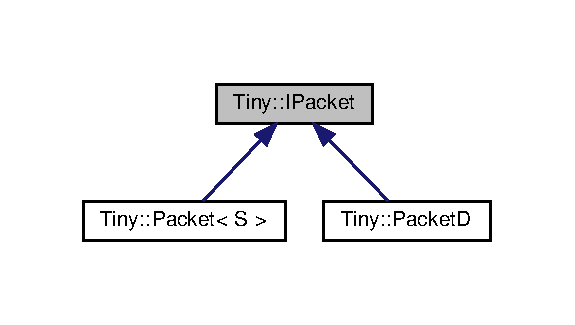
\includegraphics[width=276pt]{classTiny_1_1IPacket__inherit__graph}
\end{center}
\end{figure}
\subsection*{Public Member Functions}
\begin{DoxyCompactItemize}
\item 
\hyperlink{classTiny_1_1IPacket_af44b18c4c8481475d40d8b87a6cb38ff}{I\+Packet} (char $\ast$buf, size\+\_\+t \hyperlink{classTiny_1_1IPacket_a76b6389f0d47b67c8428c58c2b09df51}{size})
\item 
virtual \hyperlink{classTiny_1_1IPacket_a187fce5726b428db3a36e62522472c5b}{$\sim$\+I\+Packet} ()=default
\item 
void \hyperlink{classTiny_1_1IPacket_a6cc28c5235de6a9ce68bea546a4db17c}{clear} ()
\item 
void \hyperlink{classTiny_1_1IPacket_a9d5ba62a453b9cd364c0e214c245f11d}{put} (uint8\+\_\+t byte)
\item 
void \hyperlink{classTiny_1_1IPacket_a9dd0344bbed4500af63a3f700d31945b}{put} (char chr)
\item 
void \hyperlink{classTiny_1_1IPacket_a4dd6118251a5557691e4ed358a3b2ddc}{put} (uint16\+\_\+t \hyperlink{classTiny_1_1IPacket_aedf2ba31c5a29e3829458bd9f03a7051}{data})
\item 
void \hyperlink{classTiny_1_1IPacket_a5ec37c88a536d710fb1561cd62f52c91}{put} (uint32\+\_\+t \hyperlink{classTiny_1_1IPacket_aedf2ba31c5a29e3829458bd9f03a7051}{data})
\item 
void \hyperlink{classTiny_1_1IPacket_abf21aef6652da2e975c8be13e6a643e9}{put} (int16\+\_\+t \hyperlink{classTiny_1_1IPacket_aedf2ba31c5a29e3829458bd9f03a7051}{data})
\item 
void \hyperlink{classTiny_1_1IPacket_a46eaf3eb0232288dfb36ce7cc01b12e5}{put} (const char $\ast$str)
\item 
void \hyperlink{classTiny_1_1IPacket_a5ebc1e6507e7255a8babddbae82dcb2a}{put} (const \hyperlink{classTiny_1_1IPacket}{I\+Packet} \&pkt)
\item 
uint8\+\_\+t \hyperlink{classTiny_1_1IPacket_ac3088a86a37df4d08d0f6ca961abf006}{get\+Byte} ()
\item 
char \hyperlink{classTiny_1_1IPacket_a0fea05a806c533be32c68bb3899bd596}{get\+Char} ()
\item 
uint16\+\_\+t \hyperlink{classTiny_1_1IPacket_a345d5d5791d5929c9a5f9bb2763f99a5}{get\+Uint16} ()
\item 
int16\+\_\+t \hyperlink{classTiny_1_1IPacket_a9fd3b560b1f34e5d4c3e4a856bddc293}{get\+Int16} ()
\item 
uint32\+\_\+t \hyperlink{classTiny_1_1IPacket_a0a0d3758ca0f61e3eee9d20a7142de8d}{get\+Uint32} ()
\item 
char $\ast$ \hyperlink{classTiny_1_1IPacket_ac6e6a22ce9a652954491a8d4db081d79}{get\+String} ()
\item 
size\+\_\+t \hyperlink{classTiny_1_1IPacket_a76b6389f0d47b67c8428c58c2b09df51}{size} () const
\item 
size\+\_\+t \hyperlink{classTiny_1_1IPacket_a0a448d8efe2b6db3ee826f23b184b395}{max\+Size} () const
\item 
char $\ast$ \hyperlink{classTiny_1_1IPacket_aedf2ba31c5a29e3829458bd9f03a7051}{data} ()
\item 
uint8\+\_\+t \& \hyperlink{classTiny_1_1IPacket_aa1d796806e21d1c72a1fc12d2f6db592}{operator\mbox{[}$\,$\mbox{]}} (size\+\_\+t idx)
\end{DoxyCompactItemize}
\subsection*{Friends}
\begin{DoxyCompactItemize}
\item 
\mbox{\Hypertarget{classTiny_1_1IPacket_a7f90e063a34c3417ed1ea25e64608857}\label{classTiny_1_1IPacket_a7f90e063a34c3417ed1ea25e64608857}} 
class {\bfseries Proto\+Hd}
\item 
\mbox{\Hypertarget{classTiny_1_1IPacket_acb64e0550d8886dc8b8b5f1393667578}\label{classTiny_1_1IPacket_acb64e0550d8886dc8b8b5f1393667578}} 
class {\bfseries I\+Proto\+Fd}
\item 
\mbox{\Hypertarget{classTiny_1_1IPacket_a1d317236f2a79fa559d5a9112e555882}\label{classTiny_1_1IPacket_a1d317236f2a79fa559d5a9112e555882}} 
class {\bfseries Proto\+Light}
\end{DoxyCompactItemize}


\subsection{Detailed Description}
Describes packet entity and provides A\+PI methods to manipulate the packet. 

\subsection{Constructor \& Destructor Documentation}
\mbox{\Hypertarget{classTiny_1_1IPacket_af44b18c4c8481475d40d8b87a6cb38ff}\label{classTiny_1_1IPacket_af44b18c4c8481475d40d8b87a6cb38ff}} 
\index{Tiny\+::\+I\+Packet@{Tiny\+::\+I\+Packet}!I\+Packet@{I\+Packet}}
\index{I\+Packet@{I\+Packet}!Tiny\+::\+I\+Packet@{Tiny\+::\+I\+Packet}}
\subsubsection{\texorpdfstring{I\+Packet()}{IPacket()}}
{\footnotesize\ttfamily Tiny\+::\+I\+Packet\+::\+I\+Packet (\begin{DoxyParamCaption}\item[{char $\ast$}]{buf,  }\item[{size\+\_\+t}]{size }\end{DoxyParamCaption})\hspace{0.3cm}{\ttfamily [inline]}}

Creates packet object. 
\begin{DoxyParams}{Parameters}
{\em buf} & -\/ pointer to the buffer to store packet data \\
\hline
{\em size} & -\/ size of the buffer to hold packet data \\
\hline
\end{DoxyParams}
\begin{DoxyNote}{Note}
passed buffer must exist all lifecycle of the \hyperlink{classTiny_1_1Packet}{Packet} object. 
\end{DoxyNote}
\mbox{\Hypertarget{classTiny_1_1IPacket_a187fce5726b428db3a36e62522472c5b}\label{classTiny_1_1IPacket_a187fce5726b428db3a36e62522472c5b}} 
\index{Tiny\+::\+I\+Packet@{Tiny\+::\+I\+Packet}!````~I\+Packet@{$\sim$\+I\+Packet}}
\index{````~I\+Packet@{$\sim$\+I\+Packet}!Tiny\+::\+I\+Packet@{Tiny\+::\+I\+Packet}}
\subsubsection{\texorpdfstring{$\sim$\+I\+Packet()}{~IPacket()}}
{\footnotesize\ttfamily virtual Tiny\+::\+I\+Packet\+::$\sim$\+I\+Packet (\begin{DoxyParamCaption}{ }\end{DoxyParamCaption})\hspace{0.3cm}{\ttfamily [virtual]}, {\ttfamily [default]}}

Destroys the object 

\subsection{Member Function Documentation}
\mbox{\Hypertarget{classTiny_1_1IPacket_a6cc28c5235de6a9ce68bea546a4db17c}\label{classTiny_1_1IPacket_a6cc28c5235de6a9ce68bea546a4db17c}} 
\index{Tiny\+::\+I\+Packet@{Tiny\+::\+I\+Packet}!clear@{clear}}
\index{clear@{clear}!Tiny\+::\+I\+Packet@{Tiny\+::\+I\+Packet}}
\subsubsection{\texorpdfstring{clear()}{clear()}}
{\footnotesize\ttfamily void Tiny\+::\+I\+Packet\+::clear (\begin{DoxyParamCaption}{ }\end{DoxyParamCaption})\hspace{0.3cm}{\ttfamily [inline]}}

Clears \hyperlink{classTiny_1_1Packet}{Packet} state. Buffer and its size are preserved. \mbox{\Hypertarget{classTiny_1_1IPacket_aedf2ba31c5a29e3829458bd9f03a7051}\label{classTiny_1_1IPacket_aedf2ba31c5a29e3829458bd9f03a7051}} 
\index{Tiny\+::\+I\+Packet@{Tiny\+::\+I\+Packet}!data@{data}}
\index{data@{data}!Tiny\+::\+I\+Packet@{Tiny\+::\+I\+Packet}}
\subsubsection{\texorpdfstring{data()}{data()}}
{\footnotesize\ttfamily char$\ast$ Tiny\+::\+I\+Packet\+::data (\begin{DoxyParamCaption}{ }\end{DoxyParamCaption})\hspace{0.3cm}{\ttfamily [inline]}}

Returns size of payload data in the received packet. \begin{DoxyReturn}{Returns}
size of payload data. 
\end{DoxyReturn}
\mbox{\Hypertarget{classTiny_1_1IPacket_ac3088a86a37df4d08d0f6ca961abf006}\label{classTiny_1_1IPacket_ac3088a86a37df4d08d0f6ca961abf006}} 
\index{Tiny\+::\+I\+Packet@{Tiny\+::\+I\+Packet}!get\+Byte@{get\+Byte}}
\index{get\+Byte@{get\+Byte}!Tiny\+::\+I\+Packet@{Tiny\+::\+I\+Packet}}
\subsubsection{\texorpdfstring{get\+Byte()}{getByte()}}
{\footnotesize\ttfamily uint8\+\_\+t Tiny\+::\+I\+Packet\+::get\+Byte (\begin{DoxyParamCaption}{ }\end{DoxyParamCaption})\hspace{0.3cm}{\ttfamily [inline]}}

Reads next byte from the packet. \begin{DoxyReturn}{Returns}
byte from the packet. 
\end{DoxyReturn}
\mbox{\Hypertarget{classTiny_1_1IPacket_a0fea05a806c533be32c68bb3899bd596}\label{classTiny_1_1IPacket_a0fea05a806c533be32c68bb3899bd596}} 
\index{Tiny\+::\+I\+Packet@{Tiny\+::\+I\+Packet}!get\+Char@{get\+Char}}
\index{get\+Char@{get\+Char}!Tiny\+::\+I\+Packet@{Tiny\+::\+I\+Packet}}
\subsubsection{\texorpdfstring{get\+Char()}{getChar()}}
{\footnotesize\ttfamily char Tiny\+::\+I\+Packet\+::get\+Char (\begin{DoxyParamCaption}{ }\end{DoxyParamCaption})\hspace{0.3cm}{\ttfamily [inline]}}

Reads next character from the packet. \begin{DoxyReturn}{Returns}
character from the packet. 
\end{DoxyReturn}
\mbox{\Hypertarget{classTiny_1_1IPacket_a9fd3b560b1f34e5d4c3e4a856bddc293}\label{classTiny_1_1IPacket_a9fd3b560b1f34e5d4c3e4a856bddc293}} 
\index{Tiny\+::\+I\+Packet@{Tiny\+::\+I\+Packet}!get\+Int16@{get\+Int16}}
\index{get\+Int16@{get\+Int16}!Tiny\+::\+I\+Packet@{Tiny\+::\+I\+Packet}}
\subsubsection{\texorpdfstring{get\+Int16()}{getInt16()}}
{\footnotesize\ttfamily int16\+\_\+t Tiny\+::\+I\+Packet\+::get\+Int16 (\begin{DoxyParamCaption}{ }\end{DoxyParamCaption})\hspace{0.3cm}{\ttfamily [inline]}}

Reads next signed 16-\/bit integer from the packet. \begin{DoxyReturn}{Returns}
signed 16-\/bit integer. 
\end{DoxyReturn}
\mbox{\Hypertarget{classTiny_1_1IPacket_ac6e6a22ce9a652954491a8d4db081d79}\label{classTiny_1_1IPacket_ac6e6a22ce9a652954491a8d4db081d79}} 
\index{Tiny\+::\+I\+Packet@{Tiny\+::\+I\+Packet}!get\+String@{get\+String}}
\index{get\+String@{get\+String}!Tiny\+::\+I\+Packet@{Tiny\+::\+I\+Packet}}
\subsubsection{\texorpdfstring{get\+String()}{getString()}}
{\footnotesize\ttfamily char$\ast$ Tiny\+::\+I\+Packet\+::get\+String (\begin{DoxyParamCaption}{ }\end{DoxyParamCaption})\hspace{0.3cm}{\ttfamily [inline]}}

Reads zero-\/terminated string from the packet. \begin{DoxyReturn}{Returns}
zero-\/terminated string. 
\end{DoxyReturn}
\mbox{\Hypertarget{classTiny_1_1IPacket_a345d5d5791d5929c9a5f9bb2763f99a5}\label{classTiny_1_1IPacket_a345d5d5791d5929c9a5f9bb2763f99a5}} 
\index{Tiny\+::\+I\+Packet@{Tiny\+::\+I\+Packet}!get\+Uint16@{get\+Uint16}}
\index{get\+Uint16@{get\+Uint16}!Tiny\+::\+I\+Packet@{Tiny\+::\+I\+Packet}}
\subsubsection{\texorpdfstring{get\+Uint16()}{getUint16()}}
{\footnotesize\ttfamily uint16\+\_\+t Tiny\+::\+I\+Packet\+::get\+Uint16 (\begin{DoxyParamCaption}{ }\end{DoxyParamCaption})\hspace{0.3cm}{\ttfamily [inline]}}

Reads next unsigned 16-\/bit integer from the packet. \begin{DoxyReturn}{Returns}
unsigned 16-\/bit integer. 
\end{DoxyReturn}
\mbox{\Hypertarget{classTiny_1_1IPacket_a0a0d3758ca0f61e3eee9d20a7142de8d}\label{classTiny_1_1IPacket_a0a0d3758ca0f61e3eee9d20a7142de8d}} 
\index{Tiny\+::\+I\+Packet@{Tiny\+::\+I\+Packet}!get\+Uint32@{get\+Uint32}}
\index{get\+Uint32@{get\+Uint32}!Tiny\+::\+I\+Packet@{Tiny\+::\+I\+Packet}}
\subsubsection{\texorpdfstring{get\+Uint32()}{getUint32()}}
{\footnotesize\ttfamily uint32\+\_\+t Tiny\+::\+I\+Packet\+::get\+Uint32 (\begin{DoxyParamCaption}{ }\end{DoxyParamCaption})\hspace{0.3cm}{\ttfamily [inline]}}

Reads next unsigned 32-\/bit integer from the packet. \begin{DoxyReturn}{Returns}
unsigned 32-\/bit integer. 
\end{DoxyReturn}
\mbox{\Hypertarget{classTiny_1_1IPacket_a0a448d8efe2b6db3ee826f23b184b395}\label{classTiny_1_1IPacket_a0a448d8efe2b6db3ee826f23b184b395}} 
\index{Tiny\+::\+I\+Packet@{Tiny\+::\+I\+Packet}!max\+Size@{max\+Size}}
\index{max\+Size@{max\+Size}!Tiny\+::\+I\+Packet@{Tiny\+::\+I\+Packet}}
\subsubsection{\texorpdfstring{max\+Size()}{maxSize()}}
{\footnotesize\ttfamily size\+\_\+t Tiny\+::\+I\+Packet\+::max\+Size (\begin{DoxyParamCaption}{ }\end{DoxyParamCaption}) const\hspace{0.3cm}{\ttfamily [inline]}}

Returns maximum size of packet buffer. \begin{DoxyReturn}{Returns}
max size of packet buffer. 
\end{DoxyReturn}
\mbox{\Hypertarget{classTiny_1_1IPacket_aa1d796806e21d1c72a1fc12d2f6db592}\label{classTiny_1_1IPacket_aa1d796806e21d1c72a1fc12d2f6db592}} 
\index{Tiny\+::\+I\+Packet@{Tiny\+::\+I\+Packet}!operator\mbox{[}\mbox{]}@{operator[]}}
\index{operator\mbox{[}\mbox{]}@{operator[]}!Tiny\+::\+I\+Packet@{Tiny\+::\+I\+Packet}}
\subsubsection{\texorpdfstring{operator[]()}{operator[]()}}
{\footnotesize\ttfamily uint8\+\_\+t\& Tiny\+::\+I\+Packet\+::operator\mbox{[}$\,$\mbox{]} (\begin{DoxyParamCaption}\item[{size\+\_\+t}]{idx }\end{DoxyParamCaption})\hspace{0.3cm}{\ttfamily [inline]}}

You may refer to \hyperlink{classTiny_1_1Packet}{Packet} payload data directly by using operator \mbox{[}\mbox{]} \mbox{\Hypertarget{classTiny_1_1IPacket_a9d5ba62a453b9cd364c0e214c245f11d}\label{classTiny_1_1IPacket_a9d5ba62a453b9cd364c0e214c245f11d}} 
\index{Tiny\+::\+I\+Packet@{Tiny\+::\+I\+Packet}!put@{put}}
\index{put@{put}!Tiny\+::\+I\+Packet@{Tiny\+::\+I\+Packet}}
\subsubsection{\texorpdfstring{put()}{put()}\hspace{0.1cm}{\footnotesize\ttfamily [1/7]}}
{\footnotesize\ttfamily void Tiny\+::\+I\+Packet\+::put (\begin{DoxyParamCaption}\item[{uint8\+\_\+t}]{byte }\end{DoxyParamCaption})\hspace{0.3cm}{\ttfamily [inline]}}

Puts next byte to the packet. For example, after calling this method twice\+: put(5), put(10), -\/ the \hyperlink{classTiny_1_1Packet}{Packet} will contain 5,10. 
\begin{DoxyParams}{Parameters}
{\em byte} & -\/ data byte to put. \\
\hline
\end{DoxyParams}
\mbox{\Hypertarget{classTiny_1_1IPacket_a9dd0344bbed4500af63a3f700d31945b}\label{classTiny_1_1IPacket_a9dd0344bbed4500af63a3f700d31945b}} 
\index{Tiny\+::\+I\+Packet@{Tiny\+::\+I\+Packet}!put@{put}}
\index{put@{put}!Tiny\+::\+I\+Packet@{Tiny\+::\+I\+Packet}}
\subsubsection{\texorpdfstring{put()}{put()}\hspace{0.1cm}{\footnotesize\ttfamily [2/7]}}
{\footnotesize\ttfamily void Tiny\+::\+I\+Packet\+::put (\begin{DoxyParamCaption}\item[{char}]{chr }\end{DoxyParamCaption})\hspace{0.3cm}{\ttfamily [inline]}}

Puts next char to the packet. For example, after calling this method twice\+: put(\textquotesingle{}a\textquotesingle{}), put(\textquotesingle{}c\textquotesingle{}), -\/ the \hyperlink{classTiny_1_1Packet}{Packet} will contain \textquotesingle{}ac\textquotesingle{}. 
\begin{DoxyParams}{Parameters}
{\em chr} & -\/ character to put. \\
\hline
\end{DoxyParams}
\mbox{\Hypertarget{classTiny_1_1IPacket_a4dd6118251a5557691e4ed358a3b2ddc}\label{classTiny_1_1IPacket_a4dd6118251a5557691e4ed358a3b2ddc}} 
\index{Tiny\+::\+I\+Packet@{Tiny\+::\+I\+Packet}!put@{put}}
\index{put@{put}!Tiny\+::\+I\+Packet@{Tiny\+::\+I\+Packet}}
\subsubsection{\texorpdfstring{put()}{put()}\hspace{0.1cm}{\footnotesize\ttfamily [3/7]}}
{\footnotesize\ttfamily void Tiny\+::\+I\+Packet\+::put (\begin{DoxyParamCaption}\item[{uint16\+\_\+t}]{data }\end{DoxyParamCaption})\hspace{0.3cm}{\ttfamily [inline]}}

Puts next 16-\/bit unsigned integer to the packet. 
\begin{DoxyParams}{Parameters}
{\em data} & -\/ data to put. \\
\hline
\end{DoxyParams}
\mbox{\Hypertarget{classTiny_1_1IPacket_a5ec37c88a536d710fb1561cd62f52c91}\label{classTiny_1_1IPacket_a5ec37c88a536d710fb1561cd62f52c91}} 
\index{Tiny\+::\+I\+Packet@{Tiny\+::\+I\+Packet}!put@{put}}
\index{put@{put}!Tiny\+::\+I\+Packet@{Tiny\+::\+I\+Packet}}
\subsubsection{\texorpdfstring{put()}{put()}\hspace{0.1cm}{\footnotesize\ttfamily [4/7]}}
{\footnotesize\ttfamily void Tiny\+::\+I\+Packet\+::put (\begin{DoxyParamCaption}\item[{uint32\+\_\+t}]{data }\end{DoxyParamCaption})\hspace{0.3cm}{\ttfamily [inline]}}

Puts next 32-\/bit unsigned integer to the packet. 
\begin{DoxyParams}{Parameters}
{\em data} & -\/ data to put. \\
\hline
\end{DoxyParams}
\mbox{\Hypertarget{classTiny_1_1IPacket_abf21aef6652da2e975c8be13e6a643e9}\label{classTiny_1_1IPacket_abf21aef6652da2e975c8be13e6a643e9}} 
\index{Tiny\+::\+I\+Packet@{Tiny\+::\+I\+Packet}!put@{put}}
\index{put@{put}!Tiny\+::\+I\+Packet@{Tiny\+::\+I\+Packet}}
\subsubsection{\texorpdfstring{put()}{put()}\hspace{0.1cm}{\footnotesize\ttfamily [5/7]}}
{\footnotesize\ttfamily void Tiny\+::\+I\+Packet\+::put (\begin{DoxyParamCaption}\item[{int16\+\_\+t}]{data }\end{DoxyParamCaption})\hspace{0.3cm}{\ttfamily [inline]}}

Puts next 16-\/bit signed integer to the packet. 
\begin{DoxyParams}{Parameters}
{\em data} & -\/ data to put. \\
\hline
\end{DoxyParams}
\mbox{\Hypertarget{classTiny_1_1IPacket_a46eaf3eb0232288dfb36ce7cc01b12e5}\label{classTiny_1_1IPacket_a46eaf3eb0232288dfb36ce7cc01b12e5}} 
\index{Tiny\+::\+I\+Packet@{Tiny\+::\+I\+Packet}!put@{put}}
\index{put@{put}!Tiny\+::\+I\+Packet@{Tiny\+::\+I\+Packet}}
\subsubsection{\texorpdfstring{put()}{put()}\hspace{0.1cm}{\footnotesize\ttfamily [6/7]}}
{\footnotesize\ttfamily void Tiny\+::\+I\+Packet\+::put (\begin{DoxyParamCaption}\item[{const char $\ast$}]{str }\end{DoxyParamCaption})\hspace{0.3cm}{\ttfamily [inline]}}

Puts next null-\/terminated string to the packet. 
\begin{DoxyParams}{Parameters}
{\em str} & -\/ string to put. \\
\hline
\end{DoxyParams}
\mbox{\Hypertarget{classTiny_1_1IPacket_a5ebc1e6507e7255a8babddbae82dcb2a}\label{classTiny_1_1IPacket_a5ebc1e6507e7255a8babddbae82dcb2a}} 
\index{Tiny\+::\+I\+Packet@{Tiny\+::\+I\+Packet}!put@{put}}
\index{put@{put}!Tiny\+::\+I\+Packet@{Tiny\+::\+I\+Packet}}
\subsubsection{\texorpdfstring{put()}{put()}\hspace{0.1cm}{\footnotesize\ttfamily [7/7]}}
{\footnotesize\ttfamily void Tiny\+::\+I\+Packet\+::put (\begin{DoxyParamCaption}\item[{const \hyperlink{classTiny_1_1IPacket}{I\+Packet} \&}]{pkt }\end{DoxyParamCaption})\hspace{0.3cm}{\ttfamily [inline]}}

Adds data from packet to the new packet being built. 
\begin{DoxyParams}{Parameters}
{\em pkt} & -\/ reference to the \hyperlink{classTiny_1_1Packet}{Packet} to add. \\
\hline
\end{DoxyParams}
\mbox{\Hypertarget{classTiny_1_1IPacket_a76b6389f0d47b67c8428c58c2b09df51}\label{classTiny_1_1IPacket_a76b6389f0d47b67c8428c58c2b09df51}} 
\index{Tiny\+::\+I\+Packet@{Tiny\+::\+I\+Packet}!size@{size}}
\index{size@{size}!Tiny\+::\+I\+Packet@{Tiny\+::\+I\+Packet}}
\subsubsection{\texorpdfstring{size()}{size()}}
{\footnotesize\ttfamily size\+\_\+t Tiny\+::\+I\+Packet\+::size (\begin{DoxyParamCaption}{ }\end{DoxyParamCaption}) const\hspace{0.3cm}{\ttfamily [inline]}}

Returns size of payload data in the received packet. \begin{DoxyReturn}{Returns}
size of payload data. 
\end{DoxyReturn}


The documentation for this class was generated from the following file\+:\begin{DoxyCompactItemize}
\item 
src/\hyperlink{TinyPacket_8h}{Tiny\+Packet.\+h}\end{DoxyCompactItemize}

\hypertarget{classTiny_1_1IProtoFd}{}\section{Tiny\+:\+:I\+Proto\+Fd Class Reference}
\label{classTiny_1_1IProtoFd}\index{Tiny\+::\+I\+Proto\+Fd@{Tiny\+::\+I\+Proto\+Fd}}


{\ttfamily \#include $<$Tiny\+Protocol\+Fd.\+h$>$}



Inheritance diagram for Tiny\+:\+:I\+Proto\+Fd\+:
\nopagebreak
\begin{figure}[H]
\begin{center}
\leavevmode
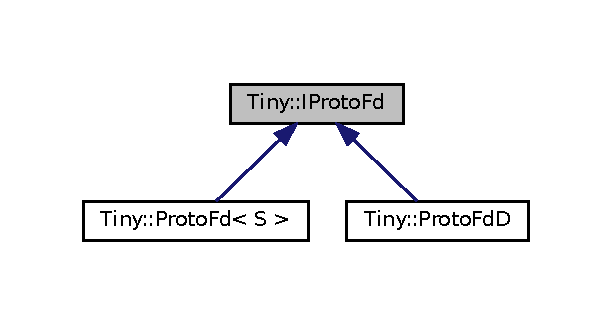
\includegraphics[width=282pt]{classTiny_1_1IProtoFd__inherit__graph}
\end{center}
\end{figure}
\subsection*{Public Member Functions}
\begin{DoxyCompactItemize}
\item 
\hyperlink{classTiny_1_1IProtoFd_a65976c6faaf41504b7c15036edc054cf}{I\+Proto\+Fd} (void $\ast$buffer, int buffer\+Size)
\item 
void \hyperlink{classTiny_1_1IProtoFd_aae4e613316866105c130d613ecb25dd4}{begin} (\hyperlink{tiny__types_8h_aafd634660bba76cace57a8f9b01e044d}{write\+\_\+block\+\_\+cb\+\_\+t} writecb, \hyperlink{tiny__types_8h_a15bec127d9ee63658563d62e92b5261b}{read\+\_\+block\+\_\+cb\+\_\+t} readcb)
\item 
void \hyperlink{classTiny_1_1IProtoFd_a1cf42b4182e49dcde4862a768d07c811}{begin\+To\+Serial} ()
\item 
void \hyperlink{classTiny_1_1IProtoFd_a7d41a0caae1d5e6808a441c821ed8927}{begin\+To\+Serial1} ()
\item 
void \hyperlink{classTiny_1_1IProtoFd_ae7582aca0fa5472da6f4ae2911d56259}{begin\+To\+Serial2} ()
\item 
void \hyperlink{classTiny_1_1IProtoFd_a2d4df949358d4e8afa391e8960729d71}{begin\+To\+Serial3} ()
\item 
void \hyperlink{classTiny_1_1IProtoFd_ad17e76d0ef7ea40838e51acc2498c482}{end} ()
\item 
int \hyperlink{classTiny_1_1IProtoFd_adea59df6702e16fd986a91c7ee62012a}{write} (char $\ast$buf, int size)
\item 
int \hyperlink{classTiny_1_1IProtoFd_aa822a1dec320e6edc70a84699371fe81}{write} (\hyperlink{classTiny_1_1IPacket}{I\+Packet} \&pkt)
\item 
int \hyperlink{classTiny_1_1IProtoFd_a37292eb5c9faf1be8c4850985e0ae2eb}{run\+\_\+rx} (uint16\+\_\+t timeout=0)
\item 
int \hyperlink{classTiny_1_1IProtoFd_a19be0bd5124009c7de051554841070b3}{run\+\_\+tx} (uint16\+\_\+t timeout=0)
\item 
void \hyperlink{classTiny_1_1IProtoFd_af41446f47a7c520ff8f9683e6ae45614}{disable\+Crc} ()
\item 
void \hyperlink{classTiny_1_1IProtoFd_a7dec2906051505034e91b503318a5563}{enable\+Crc} (\hyperlink{group__HDLC__API_gabb73b32d08d8e79eefe9385634a74bf7}{hdlc\+\_\+crc\+\_\+t} crc)
\item 
bool \hyperlink{classTiny_1_1IProtoFd_a0f43402e86ea64f5c0154477d84b0c7c}{enable\+Check\+Sum} ()
\item 
bool \hyperlink{classTiny_1_1IProtoFd_a8b57afdb66434aa35409af34b04e1db9}{enable\+Crc16} ()
\item 
bool \hyperlink{classTiny_1_1IProtoFd_a1bf1f5211ae3a49caf73ee3de3bb9247}{enable\+Crc32} ()
\item 
void \hyperlink{classTiny_1_1IProtoFd_a70aa7c85b5fe83513eebb63b803d5825}{set\+Receive\+Callback} (void($\ast$on\+\_\+receive)(\hyperlink{classTiny_1_1IPacket}{I\+Packet} \&pkt)=nullptr)
\item 
void \hyperlink{classTiny_1_1IProtoFd_adddcc24bf1ef40d39c944679a97c1ec4}{set\+Window\+Size} (uint8\+\_\+t window)
\item 
void \hyperlink{classTiny_1_1IProtoFd_a2492655abda41d5b0fbda6f0e1c6badc}{set\+Send\+Timeout} (uint16\+\_\+t timeout)
\end{DoxyCompactItemize}
\subsection*{Protected Member Functions}
\begin{DoxyCompactItemize}
\item 
virtual void \hyperlink{classTiny_1_1IProtoFd_a795b41c969708964cd4646580af1c3ab}{on\+Receive} (uint8\+\_\+t $\ast$pdata, int size)
\end{DoxyCompactItemize}
\subsection*{Friends}
\begin{DoxyCompactItemize}
\item 
\mbox{\Hypertarget{classTiny_1_1IProtoFd_ac4b680549c66e93cb1996fadcf86d724}\label{classTiny_1_1IProtoFd_ac4b680549c66e93cb1996fadcf86d724}} 
class {\bfseries Proto\+FdD}
\end{DoxyCompactItemize}


\subsection{Detailed Description}
\hyperlink{classTiny_1_1IProtoFd}{I\+Proto\+Fd} class incapsulates Full Duplex Protocol functionality. Full Duplex version of the Protocol allows to send messages with confirmation. Remember that you may use always C-\/style A\+PI functions instead C++. Please refer to documentation. 

\subsection{Constructor \& Destructor Documentation}
\mbox{\Hypertarget{classTiny_1_1IProtoFd_a65976c6faaf41504b7c15036edc054cf}\label{classTiny_1_1IProtoFd_a65976c6faaf41504b7c15036edc054cf}} 
\index{Tiny\+::\+I\+Proto\+Fd@{Tiny\+::\+I\+Proto\+Fd}!I\+Proto\+Fd@{I\+Proto\+Fd}}
\index{I\+Proto\+Fd@{I\+Proto\+Fd}!Tiny\+::\+I\+Proto\+Fd@{Tiny\+::\+I\+Proto\+Fd}}
\subsubsection{\texorpdfstring{I\+Proto\+Fd()}{IProtoFd()}}
{\footnotesize\ttfamily Tiny\+::\+I\+Proto\+Fd\+::\+I\+Proto\+Fd (\begin{DoxyParamCaption}\item[{void $\ast$}]{buffer,  }\item[{int}]{buffer\+Size }\end{DoxyParamCaption})\hspace{0.3cm}{\ttfamily [inline]}}

Initializes \hyperlink{classTiny_1_1IProtoFd}{I\+Proto\+Fd} object 
\begin{DoxyParams}{Parameters}
{\em buffer} & -\/ buffer to store the frames being received. \\
\hline
{\em buffer\+Size} & -\/ size of the buffer \\
\hline
\end{DoxyParams}


\subsection{Member Function Documentation}
\mbox{\Hypertarget{classTiny_1_1IProtoFd_aae4e613316866105c130d613ecb25dd4}\label{classTiny_1_1IProtoFd_aae4e613316866105c130d613ecb25dd4}} 
\index{Tiny\+::\+I\+Proto\+Fd@{Tiny\+::\+I\+Proto\+Fd}!begin@{begin}}
\index{begin@{begin}!Tiny\+::\+I\+Proto\+Fd@{Tiny\+::\+I\+Proto\+Fd}}
\subsubsection{\texorpdfstring{begin()}{begin()}}
{\footnotesize\ttfamily void Tiny\+::\+I\+Proto\+Fd\+::begin (\begin{DoxyParamCaption}\item[{\hyperlink{tiny__types_8h_aafd634660bba76cace57a8f9b01e044d}{write\+\_\+block\+\_\+cb\+\_\+t}}]{writecb,  }\item[{\hyperlink{tiny__types_8h_a15bec127d9ee63658563d62e92b5261b}{read\+\_\+block\+\_\+cb\+\_\+t}}]{readcb }\end{DoxyParamCaption})}

Initializes protocol internal variables. If you need to switch communication with other destination point, you can call this method one again after calling \hyperlink{classTiny_1_1IProtoFd_ad17e76d0ef7ea40838e51acc2498c482}{end()}. 
\begin{DoxyParams}{Parameters}
{\em writecb} & -\/ write function to some physical channel \\
\hline
{\em readcb} & -\/ read function from some physical channel \\
\hline
\end{DoxyParams}
\begin{DoxyReturn}{Returns}
None 
\end{DoxyReturn}
\mbox{\Hypertarget{classTiny_1_1IProtoFd_a1cf42b4182e49dcde4862a768d07c811}\label{classTiny_1_1IProtoFd_a1cf42b4182e49dcde4862a768d07c811}} 
\index{Tiny\+::\+I\+Proto\+Fd@{Tiny\+::\+I\+Proto\+Fd}!begin\+To\+Serial@{begin\+To\+Serial}}
\index{begin\+To\+Serial@{begin\+To\+Serial}!Tiny\+::\+I\+Proto\+Fd@{Tiny\+::\+I\+Proto\+Fd}}
\subsubsection{\texorpdfstring{begin\+To\+Serial()}{beginToSerial()}}
{\footnotesize\ttfamily void Tiny\+::\+I\+Proto\+Fd\+::begin\+To\+Serial (\begin{DoxyParamCaption}{ }\end{DoxyParamCaption})\hspace{0.3cm}{\ttfamily [inline]}}

Initializes protocol internal variables and redirects communication through Arduino Serial connection (Serial). \begin{DoxyReturn}{Returns}
None 
\end{DoxyReturn}
\mbox{\Hypertarget{classTiny_1_1IProtoFd_a7d41a0caae1d5e6808a441c821ed8927}\label{classTiny_1_1IProtoFd_a7d41a0caae1d5e6808a441c821ed8927}} 
\index{Tiny\+::\+I\+Proto\+Fd@{Tiny\+::\+I\+Proto\+Fd}!begin\+To\+Serial1@{begin\+To\+Serial1}}
\index{begin\+To\+Serial1@{begin\+To\+Serial1}!Tiny\+::\+I\+Proto\+Fd@{Tiny\+::\+I\+Proto\+Fd}}
\subsubsection{\texorpdfstring{begin\+To\+Serial1()}{beginToSerial1()}}
{\footnotesize\ttfamily void Tiny\+::\+I\+Proto\+Fd\+::begin\+To\+Serial1 (\begin{DoxyParamCaption}{ }\end{DoxyParamCaption})\hspace{0.3cm}{\ttfamily [inline]}}

Initializes protocol internal variables and redirects communication through Arduino Serial1 connection (Serial1). \begin{DoxyReturn}{Returns}
None 
\end{DoxyReturn}
\mbox{\Hypertarget{classTiny_1_1IProtoFd_ae7582aca0fa5472da6f4ae2911d56259}\label{classTiny_1_1IProtoFd_ae7582aca0fa5472da6f4ae2911d56259}} 
\index{Tiny\+::\+I\+Proto\+Fd@{Tiny\+::\+I\+Proto\+Fd}!begin\+To\+Serial2@{begin\+To\+Serial2}}
\index{begin\+To\+Serial2@{begin\+To\+Serial2}!Tiny\+::\+I\+Proto\+Fd@{Tiny\+::\+I\+Proto\+Fd}}
\subsubsection{\texorpdfstring{begin\+To\+Serial2()}{beginToSerial2()}}
{\footnotesize\ttfamily void Tiny\+::\+I\+Proto\+Fd\+::begin\+To\+Serial2 (\begin{DoxyParamCaption}{ }\end{DoxyParamCaption})\hspace{0.3cm}{\ttfamily [inline]}}

Initializes protocol internal variables and redirects communication through Arduino Serial2 connection (Serial2). \begin{DoxyReturn}{Returns}
None 
\end{DoxyReturn}
\mbox{\Hypertarget{classTiny_1_1IProtoFd_a2d4df949358d4e8afa391e8960729d71}\label{classTiny_1_1IProtoFd_a2d4df949358d4e8afa391e8960729d71}} 
\index{Tiny\+::\+I\+Proto\+Fd@{Tiny\+::\+I\+Proto\+Fd}!begin\+To\+Serial3@{begin\+To\+Serial3}}
\index{begin\+To\+Serial3@{begin\+To\+Serial3}!Tiny\+::\+I\+Proto\+Fd@{Tiny\+::\+I\+Proto\+Fd}}
\subsubsection{\texorpdfstring{begin\+To\+Serial3()}{beginToSerial3()}}
{\footnotesize\ttfamily void Tiny\+::\+I\+Proto\+Fd\+::begin\+To\+Serial3 (\begin{DoxyParamCaption}{ }\end{DoxyParamCaption})\hspace{0.3cm}{\ttfamily [inline]}}

Initializes protocol internal variables and redirects communication through Arduino Serial3 connection (Serial3). \begin{DoxyReturn}{Returns}
None 
\end{DoxyReturn}
\mbox{\Hypertarget{classTiny_1_1IProtoFd_af41446f47a7c520ff8f9683e6ae45614}\label{classTiny_1_1IProtoFd_af41446f47a7c520ff8f9683e6ae45614}} 
\index{Tiny\+::\+I\+Proto\+Fd@{Tiny\+::\+I\+Proto\+Fd}!disable\+Crc@{disable\+Crc}}
\index{disable\+Crc@{disable\+Crc}!Tiny\+::\+I\+Proto\+Fd@{Tiny\+::\+I\+Proto\+Fd}}
\subsubsection{\texorpdfstring{disable\+Crc()}{disableCrc()}}
{\footnotesize\ttfamily void Tiny\+::\+I\+Proto\+Fd\+::disable\+Crc (\begin{DoxyParamCaption}{ }\end{DoxyParamCaption})}

Disable C\+RC field in the protocol. If C\+RC field is O\+FF, then the frame looks like this\+: 0x7E databytes 0x7E. \mbox{\Hypertarget{classTiny_1_1IProtoFd_a0f43402e86ea64f5c0154477d84b0c7c}\label{classTiny_1_1IProtoFd_a0f43402e86ea64f5c0154477d84b0c7c}} 
\index{Tiny\+::\+I\+Proto\+Fd@{Tiny\+::\+I\+Proto\+Fd}!enable\+Check\+Sum@{enable\+Check\+Sum}}
\index{enable\+Check\+Sum@{enable\+Check\+Sum}!Tiny\+::\+I\+Proto\+Fd@{Tiny\+::\+I\+Proto\+Fd}}
\subsubsection{\texorpdfstring{enable\+Check\+Sum()}{enableCheckSum()}}
{\footnotesize\ttfamily bool Tiny\+::\+I\+Proto\+Fd\+::enable\+Check\+Sum (\begin{DoxyParamCaption}{ }\end{DoxyParamCaption})}

Enables C\+RC 8-\/bit field in the protocol. This field contains sum of all data bytes in the packet. 8-\/bit field is supported by Nano version of Tiny library. \begin{DoxyReturn}{Returns}
true if successful false in case of error. 
\end{DoxyReturn}
\mbox{\Hypertarget{classTiny_1_1IProtoFd_a7dec2906051505034e91b503318a5563}\label{classTiny_1_1IProtoFd_a7dec2906051505034e91b503318a5563}} 
\index{Tiny\+::\+I\+Proto\+Fd@{Tiny\+::\+I\+Proto\+Fd}!enable\+Crc@{enable\+Crc}}
\index{enable\+Crc@{enable\+Crc}!Tiny\+::\+I\+Proto\+Fd@{Tiny\+::\+I\+Proto\+Fd}}
\subsubsection{\texorpdfstring{enable\+Crc()}{enableCrc()}}
{\footnotesize\ttfamily void Tiny\+::\+I\+Proto\+Fd\+::enable\+Crc (\begin{DoxyParamCaption}\item[{\hyperlink{group__HDLC__API_gabb73b32d08d8e79eefe9385634a74bf7}{hdlc\+\_\+crc\+\_\+t}}]{crc }\end{DoxyParamCaption})}

Enables C\+RC by specified bit-\/size. 8-\/bit is supported by Nano version of Tiny library. 
\begin{DoxyParams}{Parameters}
{\em crc} & crc type \\
\hline
\end{DoxyParams}
\mbox{\Hypertarget{classTiny_1_1IProtoFd_a8b57afdb66434aa35409af34b04e1db9}\label{classTiny_1_1IProtoFd_a8b57afdb66434aa35409af34b04e1db9}} 
\index{Tiny\+::\+I\+Proto\+Fd@{Tiny\+::\+I\+Proto\+Fd}!enable\+Crc16@{enable\+Crc16}}
\index{enable\+Crc16@{enable\+Crc16}!Tiny\+::\+I\+Proto\+Fd@{Tiny\+::\+I\+Proto\+Fd}}
\subsubsection{\texorpdfstring{enable\+Crc16()}{enableCrc16()}}
{\footnotesize\ttfamily bool Tiny\+::\+I\+Proto\+Fd\+::enable\+Crc16 (\begin{DoxyParamCaption}{ }\end{DoxyParamCaption})}

Enables C\+RC 16-\/bit field in the protocol. This field contains F\+CS 16-\/bit C\+C\+I\+TT like defined in R\+FC 1662. 16-\/bit field is not supported by Nano version of Tiny library. \begin{DoxyReturn}{Returns}
true if successful false in case of error. 
\end{DoxyReturn}
\mbox{\Hypertarget{classTiny_1_1IProtoFd_a1bf1f5211ae3a49caf73ee3de3bb9247}\label{classTiny_1_1IProtoFd_a1bf1f5211ae3a49caf73ee3de3bb9247}} 
\index{Tiny\+::\+I\+Proto\+Fd@{Tiny\+::\+I\+Proto\+Fd}!enable\+Crc32@{enable\+Crc32}}
\index{enable\+Crc32@{enable\+Crc32}!Tiny\+::\+I\+Proto\+Fd@{Tiny\+::\+I\+Proto\+Fd}}
\subsubsection{\texorpdfstring{enable\+Crc32()}{enableCrc32()}}
{\footnotesize\ttfamily bool Tiny\+::\+I\+Proto\+Fd\+::enable\+Crc32 (\begin{DoxyParamCaption}{ }\end{DoxyParamCaption})}

Enables C\+RC 32-\/bit field in the protocol. This field contains F\+CS 32-\/bit C\+C\+I\+TT like defined in R\+FC 1662. 32-\/bit field is not supported by Nano version of Tiny library. \begin{DoxyReturn}{Returns}
true if successful false in case of error. 
\end{DoxyReturn}
\mbox{\Hypertarget{classTiny_1_1IProtoFd_ad17e76d0ef7ea40838e51acc2498c482}\label{classTiny_1_1IProtoFd_ad17e76d0ef7ea40838e51acc2498c482}} 
\index{Tiny\+::\+I\+Proto\+Fd@{Tiny\+::\+I\+Proto\+Fd}!end@{end}}
\index{end@{end}!Tiny\+::\+I\+Proto\+Fd@{Tiny\+::\+I\+Proto\+Fd}}
\subsubsection{\texorpdfstring{end()}{end()}}
{\footnotesize\ttfamily void Tiny\+::\+I\+Proto\+Fd\+::end (\begin{DoxyParamCaption}{ }\end{DoxyParamCaption})}

Resets protocol state. \mbox{\Hypertarget{classTiny_1_1IProtoFd_a795b41c969708964cd4646580af1c3ab}\label{classTiny_1_1IProtoFd_a795b41c969708964cd4646580af1c3ab}} 
\index{Tiny\+::\+I\+Proto\+Fd@{Tiny\+::\+I\+Proto\+Fd}!on\+Receive@{on\+Receive}}
\index{on\+Receive@{on\+Receive}!Tiny\+::\+I\+Proto\+Fd@{Tiny\+::\+I\+Proto\+Fd}}
\subsubsection{\texorpdfstring{on\+Receive()}{onReceive()}}
{\footnotesize\ttfamily virtual void Tiny\+::\+I\+Proto\+Fd\+::on\+Receive (\begin{DoxyParamCaption}\item[{uint8\+\_\+t $\ast$}]{pdata,  }\item[{int}]{size }\end{DoxyParamCaption})\hspace{0.3cm}{\ttfamily [inline]}, {\ttfamily [protected]}, {\ttfamily [virtual]}}

Method called by hdlc protocol upon receiving new frame. Can be redefined in derived classes. 
\begin{DoxyParams}{Parameters}
{\em pdata} & pointer to received data \\
\hline
{\em size} & size of received payload in bytes \\
\hline
\end{DoxyParams}
\mbox{\Hypertarget{classTiny_1_1IProtoFd_a37292eb5c9faf1be8c4850985e0ae2eb}\label{classTiny_1_1IProtoFd_a37292eb5c9faf1be8c4850985e0ae2eb}} 
\index{Tiny\+::\+I\+Proto\+Fd@{Tiny\+::\+I\+Proto\+Fd}!run\+\_\+rx@{run\+\_\+rx}}
\index{run\+\_\+rx@{run\+\_\+rx}!Tiny\+::\+I\+Proto\+Fd@{Tiny\+::\+I\+Proto\+Fd}}
\subsubsection{\texorpdfstring{run\+\_\+rx()}{run\_rx()}}
{\footnotesize\ttfamily int Tiny\+::\+I\+Proto\+Fd\+::run\+\_\+rx (\begin{DoxyParamCaption}\item[{uint16\+\_\+t}]{timeout = {\ttfamily 0} }\end{DoxyParamCaption})}

Checks communcation channel for incoming messages. \begin{DoxyReturn}{Returns}
negative value in case of error zero if nothing is read positive -\/ \hyperlink{classTiny_1_1Packet}{Packet} is successfully received 
\end{DoxyReturn}
\begin{DoxyRemark}{Remarks}
if \hyperlink{classTiny_1_1Packet}{Packet} is receive during run execution callback is called. 
\end{DoxyRemark}
\mbox{\Hypertarget{classTiny_1_1IProtoFd_a19be0bd5124009c7de051554841070b3}\label{classTiny_1_1IProtoFd_a19be0bd5124009c7de051554841070b3}} 
\index{Tiny\+::\+I\+Proto\+Fd@{Tiny\+::\+I\+Proto\+Fd}!run\+\_\+tx@{run\+\_\+tx}}
\index{run\+\_\+tx@{run\+\_\+tx}!Tiny\+::\+I\+Proto\+Fd@{Tiny\+::\+I\+Proto\+Fd}}
\subsubsection{\texorpdfstring{run\+\_\+tx()}{run\_tx()}}
{\footnotesize\ttfamily int Tiny\+::\+I\+Proto\+Fd\+::run\+\_\+tx (\begin{DoxyParamCaption}\item[{uint16\+\_\+t}]{timeout = {\ttfamily 0} }\end{DoxyParamCaption})}

Sends data to communcation channel. \begin{DoxyReturn}{Returns}
negative value in case of error 
\end{DoxyReturn}
\mbox{\Hypertarget{classTiny_1_1IProtoFd_a70aa7c85b5fe83513eebb63b803d5825}\label{classTiny_1_1IProtoFd_a70aa7c85b5fe83513eebb63b803d5825}} 
\index{Tiny\+::\+I\+Proto\+Fd@{Tiny\+::\+I\+Proto\+Fd}!set\+Receive\+Callback@{set\+Receive\+Callback}}
\index{set\+Receive\+Callback@{set\+Receive\+Callback}!Tiny\+::\+I\+Proto\+Fd@{Tiny\+::\+I\+Proto\+Fd}}
\subsubsection{\texorpdfstring{set\+Receive\+Callback()}{setReceiveCallback()}}
{\footnotesize\ttfamily void Tiny\+::\+I\+Proto\+Fd\+::set\+Receive\+Callback (\begin{DoxyParamCaption}\item[{void($\ast$)(\hyperlink{classTiny_1_1IPacket}{I\+Packet} \&pkt)}]{on\+\_\+receive = {\ttfamily nullptr} }\end{DoxyParamCaption})\hspace{0.3cm}{\ttfamily [inline]}}

Sets receive callback for incoming messages 
\begin{DoxyParams}{Parameters}
{\em on\+\_\+receive} & user callback to process incoming messages. The processing must be non-\/blocking \\
\hline
\end{DoxyParams}
\mbox{\Hypertarget{classTiny_1_1IProtoFd_a2492655abda41d5b0fbda6f0e1c6badc}\label{classTiny_1_1IProtoFd_a2492655abda41d5b0fbda6f0e1c6badc}} 
\index{Tiny\+::\+I\+Proto\+Fd@{Tiny\+::\+I\+Proto\+Fd}!set\+Send\+Timeout@{set\+Send\+Timeout}}
\index{set\+Send\+Timeout@{set\+Send\+Timeout}!Tiny\+::\+I\+Proto\+Fd@{Tiny\+::\+I\+Proto\+Fd}}
\subsubsection{\texorpdfstring{set\+Send\+Timeout()}{setSendTimeout()}}
{\footnotesize\ttfamily void Tiny\+::\+I\+Proto\+Fd\+::set\+Send\+Timeout (\begin{DoxyParamCaption}\item[{uint16\+\_\+t}]{timeout }\end{DoxyParamCaption})\hspace{0.3cm}{\ttfamily [inline]}}

Sets send timeout in milliseconds. 
\begin{DoxyParams}{Parameters}
{\em timeout} & timeout in milliseconds, \\
\hline
\end{DoxyParams}
\mbox{\Hypertarget{classTiny_1_1IProtoFd_adddcc24bf1ef40d39c944679a97c1ec4}\label{classTiny_1_1IProtoFd_adddcc24bf1ef40d39c944679a97c1ec4}} 
\index{Tiny\+::\+I\+Proto\+Fd@{Tiny\+::\+I\+Proto\+Fd}!set\+Window\+Size@{set\+Window\+Size}}
\index{set\+Window\+Size@{set\+Window\+Size}!Tiny\+::\+I\+Proto\+Fd@{Tiny\+::\+I\+Proto\+Fd}}
\subsubsection{\texorpdfstring{set\+Window\+Size()}{setWindowSize()}}
{\footnotesize\ttfamily void Tiny\+::\+I\+Proto\+Fd\+::set\+Window\+Size (\begin{DoxyParamCaption}\item[{uint8\+\_\+t}]{window }\end{DoxyParamCaption})\hspace{0.3cm}{\ttfamily [inline]}}

Sets desired window size. Use this function only before \hyperlink{classTiny_1_1IProtoFd_aae4e613316866105c130d613ecb25dd4}{begin()} call. window size is number of frames, which confirmation may be deferred for. 
\begin{DoxyParams}{Parameters}
{\em window} & window size, valid between 1 -\/ 7 inclusively \\
\hline
\end{DoxyParams}
\begin{DoxyWarning}{Warning}
if you use smallest window size, this can reduce throughput of the channel. 
\end{DoxyWarning}
\mbox{\Hypertarget{classTiny_1_1IProtoFd_adea59df6702e16fd986a91c7ee62012a}\label{classTiny_1_1IProtoFd_adea59df6702e16fd986a91c7ee62012a}} 
\index{Tiny\+::\+I\+Proto\+Fd@{Tiny\+::\+I\+Proto\+Fd}!write@{write}}
\index{write@{write}!Tiny\+::\+I\+Proto\+Fd@{Tiny\+::\+I\+Proto\+Fd}}
\subsubsection{\texorpdfstring{write()}{write()}\hspace{0.1cm}{\footnotesize\ttfamily [1/2]}}
{\footnotesize\ttfamily int Tiny\+::\+I\+Proto\+Fd\+::write (\begin{DoxyParamCaption}\item[{char $\ast$}]{buf,  }\item[{int}]{size }\end{DoxyParamCaption})}

Sends data block over communication channel. 
\begin{DoxyParams}{Parameters}
{\em buf} & -\/ data to send \\
\hline
{\em size} & -\/ length of the data in bytes \\
\hline
\end{DoxyParams}
\begin{DoxyReturn}{Returns}
negative value in case of error zero if nothing is sent positive -\/ should be equal to size parameter 
\end{DoxyReturn}
\mbox{\Hypertarget{classTiny_1_1IProtoFd_aa822a1dec320e6edc70a84699371fe81}\label{classTiny_1_1IProtoFd_aa822a1dec320e6edc70a84699371fe81}} 
\index{Tiny\+::\+I\+Proto\+Fd@{Tiny\+::\+I\+Proto\+Fd}!write@{write}}
\index{write@{write}!Tiny\+::\+I\+Proto\+Fd@{Tiny\+::\+I\+Proto\+Fd}}
\subsubsection{\texorpdfstring{write()}{write()}\hspace{0.1cm}{\footnotesize\ttfamily [2/2]}}
{\footnotesize\ttfamily int Tiny\+::\+I\+Proto\+Fd\+::write (\begin{DoxyParamCaption}\item[{\hyperlink{classTiny_1_1IPacket}{I\+Packet} \&}]{pkt }\end{DoxyParamCaption})}

Sends packet over communication channel. 
\begin{DoxyParams}{Parameters}
{\em pkt} & -\/ \hyperlink{classTiny_1_1Packet}{Packet} to send \\
\hline
\end{DoxyParams}
\begin{DoxySeeAlso}{See also}
\hyperlink{classTiny_1_1Packet}{Packet} 
\end{DoxySeeAlso}
\begin{DoxyReturn}{Returns}
negative value in case of error zero if nothing is sent positive -\/ \hyperlink{classTiny_1_1Packet}{Packet} is successfully sent 
\end{DoxyReturn}


The documentation for this class was generated from the following file\+:\begin{DoxyCompactItemize}
\item 
src/\hyperlink{TinyProtocolFd_8h}{Tiny\+Protocol\+Fd.\+h}\end{DoxyCompactItemize}

\hypertarget{structlist__element__}{}\section{list\+\_\+element\+\_\+ Struct Reference}
\label{structlist__element__}\index{list\+\_\+element\+\_\+@{list\+\_\+element\+\_\+}}


structure defines base type for the lists  




{\ttfamily \#include $<$tiny\+\_\+list.\+h$>$}



Collaboration diagram for list\+\_\+element\+\_\+\+:\nopagebreak
\begin{figure}[H]
\begin{center}
\leavevmode
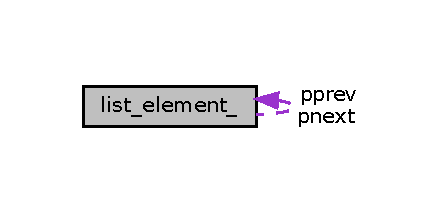
\includegraphics[width=200pt]{structlist__element____coll__graph}
\end{center}
\end{figure}
\subsection*{Public Attributes}
\begin{DoxyCompactItemize}
\item 
\hypertarget{structlist__element___a81cb2c54606be8120460bded0d919039}{}struct \hyperlink{structlist__element__}{list\+\_\+element\+\_\+} $\ast$ \hyperlink{structlist__element___a81cb2c54606be8120460bded0d919039}{pnext}\label{structlist__element___a81cb2c54606be8120460bded0d919039}

\begin{DoxyCompactList}\small\item\em pointer to the next element in the list \end{DoxyCompactList}\item 
\hypertarget{structlist__element___a0f6c573966c9d70d4a2ef19b73717515}{}struct \hyperlink{structlist__element__}{list\+\_\+element\+\_\+} $\ast$ \hyperlink{structlist__element___a0f6c573966c9d70d4a2ef19b73717515}{pprev}\label{structlist__element___a0f6c573966c9d70d4a2ef19b73717515}

\begin{DoxyCompactList}\small\item\em pointer to the previous element in the list \end{DoxyCompactList}\end{DoxyCompactItemize}


\subsection{Detailed Description}
structure defines base type for the lists 

The documentation for this struct was generated from the following file\+:\begin{DoxyCompactItemize}
\item 
src/lib/tiny\+\_\+list.\+h\end{DoxyCompactItemize}

\hypertarget{classTiny_1_1Packet}{}\section{Tiny\+:\+:Packet Class Reference}
\label{classTiny_1_1Packet}\index{Tiny\+::\+Packet@{Tiny\+::\+Packet}}


{\ttfamily \#include $<$Tiny\+Packet.\+h$>$}

\subsection*{Public Member Functions}
\begin{DoxyCompactItemize}
\item 
\hyperlink{classTiny_1_1Packet_aad47b3053945b29b1b46d76b31b72960}{Packet} (char $\ast$buf, size\+\_\+t \hyperlink{classTiny_1_1Packet_a47c24d500159d2268908b10c407d8d4d}{size})
\item 
void \hyperlink{classTiny_1_1Packet_a9bfdb9244515ef3dbf1056c1e37d0902}{clear} ()
\item 
void \hyperlink{classTiny_1_1Packet_a52c746f604ee6c0e4e78902b4cf710a9}{put} (uint8\+\_\+t byte)
\item 
void \hyperlink{classTiny_1_1Packet_a6e1e5236908290f28c3b9a0818242b5b}{put} (char chr)
\item 
void \hyperlink{classTiny_1_1Packet_a0055b5d1c437104e38bf66ece8ab84ba}{put} (uint16\+\_\+t \hyperlink{classTiny_1_1Packet_a3307ba504caba9c5eee8f1f32cf1a749}{data})
\item 
void \hyperlink{classTiny_1_1Packet_aed30fc087142669b37ec99d9d6572e57}{put} (uint32\+\_\+t \hyperlink{classTiny_1_1Packet_a3307ba504caba9c5eee8f1f32cf1a749}{data})
\item 
void \hyperlink{classTiny_1_1Packet_a464ddc51642812e604ac39f775762165}{put} (int16\+\_\+t \hyperlink{classTiny_1_1Packet_a3307ba504caba9c5eee8f1f32cf1a749}{data})
\item 
void \hyperlink{classTiny_1_1Packet_a6b5880ebffa02df3a380a270809433e1}{put} (const char $\ast$str)
\item 
void \hyperlink{classTiny_1_1Packet_a5741e3aec04c9100ce00a6b702417231}{put} (const \hyperlink{classTiny_1_1Packet}{Packet} \&pkt)
\item 
void \hyperlink{classTiny_1_1Packet_ae8764bf70fd6f09df2cb15c02ce2aa30}{put\+Uid} (uint16\+\_\+t uid)
\item 
uint8\+\_\+t \hyperlink{classTiny_1_1Packet_a152feac05d3e972f614c17c36bf30513}{get\+Byte} ()
\item 
char \hyperlink{classTiny_1_1Packet_a260645f9d055da878f149a13ecd58844}{get\+Char} ()
\item 
uint16\+\_\+t \hyperlink{classTiny_1_1Packet_a71765e73adfbc67138f75c2b8ea7d74c}{get\+Uint16} ()
\item 
int16\+\_\+t \hyperlink{classTiny_1_1Packet_a7dfed04418564f93dd4d2b4e9144a861}{get\+Int16} ()
\item 
uint32\+\_\+t \hyperlink{classTiny_1_1Packet_a5dd4b89cb7224b62d4f0328c8e40f38f}{get\+Uint32} ()
\item 
char $\ast$ \hyperlink{classTiny_1_1Packet_a8bc9a3b3f41be292f9c5ac566afeb04b}{get\+String} ()
\item 
uint16\+\_\+t \hyperlink{classTiny_1_1Packet_a65e342e15b9fa3e878393d268c4e69e4}{get\+Uid} () const
\item 
size\+\_\+t \hyperlink{classTiny_1_1Packet_a47c24d500159d2268908b10c407d8d4d}{size} () const
\item 
size\+\_\+t \hyperlink{classTiny_1_1Packet_a9985ff3b48f81628a7428b1197ca9f8f}{max\+Size} () const
\item 
char $\ast$ \hyperlink{classTiny_1_1Packet_a3307ba504caba9c5eee8f1f32cf1a749}{data} ()
\item 
uint8\+\_\+t \& \hyperlink{classTiny_1_1Packet_abfaef504eb88a4db88bca3b907770fa2}{operator\mbox{[}$\,$\mbox{]}} (size\+\_\+t idx)
\item 
\hyperlink{classTiny_1_1Packet}{Packet} \& \hyperlink{classTiny_1_1Packet_a2de2c7f2c3ea6baaab462dd7e4469ecb}{operator=} (char chr)
\end{DoxyCompactItemize}
\subsection*{Friends}
\begin{DoxyCompactItemize}
\item 
\mbox{\Hypertarget{classTiny_1_1Packet_a45bd055fddab40aaf0c60bfb9e21aa6f}\label{classTiny_1_1Packet_a45bd055fddab40aaf0c60bfb9e21aa6f}} 
class {\bfseries Proto}
\item 
\mbox{\Hypertarget{classTiny_1_1Packet_a7f90e063a34c3417ed1ea25e64608857}\label{classTiny_1_1Packet_a7f90e063a34c3417ed1ea25e64608857}} 
class {\bfseries Proto\+Hd}
\item 
\mbox{\Hypertarget{classTiny_1_1Packet_a1d317236f2a79fa559d5a9112e555882}\label{classTiny_1_1Packet_a1d317236f2a79fa559d5a9112e555882}} 
class {\bfseries Proto\+Light}
\end{DoxyCompactItemize}


\subsection{Detailed Description}
Describes packet entity and provides A\+PI methods to manipulate the packet. 

\subsection{Constructor \& Destructor Documentation}
\mbox{\Hypertarget{classTiny_1_1Packet_aad47b3053945b29b1b46d76b31b72960}\label{classTiny_1_1Packet_aad47b3053945b29b1b46d76b31b72960}} 
\index{Tiny\+::\+Packet@{Tiny\+::\+Packet}!Packet@{Packet}}
\index{Packet@{Packet}!Tiny\+::\+Packet@{Tiny\+::\+Packet}}
\subsubsection{\texorpdfstring{Packet()}{Packet()}}
{\footnotesize\ttfamily Tiny\+::\+Packet\+::\+Packet (\begin{DoxyParamCaption}\item[{char $\ast$}]{buf,  }\item[{size\+\_\+t}]{size }\end{DoxyParamCaption})\hspace{0.3cm}{\ttfamily [inline]}}

Creates packet object. 
\begin{DoxyParams}{Parameters}
{\em buf} & -\/ pointer to the buffer to store packet data \\
\hline
{\em size} & -\/ size of the buffer to hold packet data \\
\hline
\end{DoxyParams}
\begin{DoxyNote}{Note}
passed buffer must exist all lifecycle of the \hyperlink{classTiny_1_1Packet}{Packet} object. 
\end{DoxyNote}


\subsection{Member Function Documentation}
\mbox{\Hypertarget{classTiny_1_1Packet_a9bfdb9244515ef3dbf1056c1e37d0902}\label{classTiny_1_1Packet_a9bfdb9244515ef3dbf1056c1e37d0902}} 
\index{Tiny\+::\+Packet@{Tiny\+::\+Packet}!clear@{clear}}
\index{clear@{clear}!Tiny\+::\+Packet@{Tiny\+::\+Packet}}
\subsubsection{\texorpdfstring{clear()}{clear()}}
{\footnotesize\ttfamily void Tiny\+::\+Packet\+::clear (\begin{DoxyParamCaption}{ }\end{DoxyParamCaption})\hspace{0.3cm}{\ttfamily [inline]}}

Clears \hyperlink{classTiny_1_1Packet}{Packet} state. Buffer and its size are preserved. \mbox{\Hypertarget{classTiny_1_1Packet_a3307ba504caba9c5eee8f1f32cf1a749}\label{classTiny_1_1Packet_a3307ba504caba9c5eee8f1f32cf1a749}} 
\index{Tiny\+::\+Packet@{Tiny\+::\+Packet}!data@{data}}
\index{data@{data}!Tiny\+::\+Packet@{Tiny\+::\+Packet}}
\subsubsection{\texorpdfstring{data()}{data()}}
{\footnotesize\ttfamily char$\ast$ Tiny\+::\+Packet\+::data (\begin{DoxyParamCaption}{ }\end{DoxyParamCaption})\hspace{0.3cm}{\ttfamily [inline]}}

Returns size of payload data in the received packet. \begin{DoxyReturn}{Returns}
size of payload data. 
\end{DoxyReturn}
\mbox{\Hypertarget{classTiny_1_1Packet_a152feac05d3e972f614c17c36bf30513}\label{classTiny_1_1Packet_a152feac05d3e972f614c17c36bf30513}} 
\index{Tiny\+::\+Packet@{Tiny\+::\+Packet}!get\+Byte@{get\+Byte}}
\index{get\+Byte@{get\+Byte}!Tiny\+::\+Packet@{Tiny\+::\+Packet}}
\subsubsection{\texorpdfstring{get\+Byte()}{getByte()}}
{\footnotesize\ttfamily uint8\+\_\+t Tiny\+::\+Packet\+::get\+Byte (\begin{DoxyParamCaption}{ }\end{DoxyParamCaption})\hspace{0.3cm}{\ttfamily [inline]}}

Reads next byte from the packet. \begin{DoxyReturn}{Returns}
byte from the packet. 
\end{DoxyReturn}
\mbox{\Hypertarget{classTiny_1_1Packet_a260645f9d055da878f149a13ecd58844}\label{classTiny_1_1Packet_a260645f9d055da878f149a13ecd58844}} 
\index{Tiny\+::\+Packet@{Tiny\+::\+Packet}!get\+Char@{get\+Char}}
\index{get\+Char@{get\+Char}!Tiny\+::\+Packet@{Tiny\+::\+Packet}}
\subsubsection{\texorpdfstring{get\+Char()}{getChar()}}
{\footnotesize\ttfamily char Tiny\+::\+Packet\+::get\+Char (\begin{DoxyParamCaption}{ }\end{DoxyParamCaption})\hspace{0.3cm}{\ttfamily [inline]}}

Reads next character from the packet. \begin{DoxyReturn}{Returns}
character from the packet. 
\end{DoxyReturn}
\mbox{\Hypertarget{classTiny_1_1Packet_a7dfed04418564f93dd4d2b4e9144a861}\label{classTiny_1_1Packet_a7dfed04418564f93dd4d2b4e9144a861}} 
\index{Tiny\+::\+Packet@{Tiny\+::\+Packet}!get\+Int16@{get\+Int16}}
\index{get\+Int16@{get\+Int16}!Tiny\+::\+Packet@{Tiny\+::\+Packet}}
\subsubsection{\texorpdfstring{get\+Int16()}{getInt16()}}
{\footnotesize\ttfamily int16\+\_\+t Tiny\+::\+Packet\+::get\+Int16 (\begin{DoxyParamCaption}{ }\end{DoxyParamCaption})\hspace{0.3cm}{\ttfamily [inline]}}

Reads next signed 16-\/bit integer from the packet. \begin{DoxyReturn}{Returns}
signed 16-\/bit integer. 
\end{DoxyReturn}
\mbox{\Hypertarget{classTiny_1_1Packet_a8bc9a3b3f41be292f9c5ac566afeb04b}\label{classTiny_1_1Packet_a8bc9a3b3f41be292f9c5ac566afeb04b}} 
\index{Tiny\+::\+Packet@{Tiny\+::\+Packet}!get\+String@{get\+String}}
\index{get\+String@{get\+String}!Tiny\+::\+Packet@{Tiny\+::\+Packet}}
\subsubsection{\texorpdfstring{get\+String()}{getString()}}
{\footnotesize\ttfamily char$\ast$ Tiny\+::\+Packet\+::get\+String (\begin{DoxyParamCaption}{ }\end{DoxyParamCaption})\hspace{0.3cm}{\ttfamily [inline]}}

Reads zero-\/terminated string from the packet. \begin{DoxyReturn}{Returns}
zero-\/terminated string. 
\end{DoxyReturn}
\mbox{\Hypertarget{classTiny_1_1Packet_a65e342e15b9fa3e878393d268c4e69e4}\label{classTiny_1_1Packet_a65e342e15b9fa3e878393d268c4e69e4}} 
\index{Tiny\+::\+Packet@{Tiny\+::\+Packet}!get\+Uid@{get\+Uid}}
\index{get\+Uid@{get\+Uid}!Tiny\+::\+Packet@{Tiny\+::\+Packet}}
\subsubsection{\texorpdfstring{get\+Uid()}{getUid()}}
{\footnotesize\ttfamily uint16\+\_\+t Tiny\+::\+Packet\+::get\+Uid (\begin{DoxyParamCaption}{ }\end{DoxyParamCaption}) const\hspace{0.3cm}{\ttfamily [inline]}}

Returns 16-\/bit identificator of the packet. \begin{DoxyWarning}{Warning}
uid is valid only if uid functionality is enabled in the \hyperlink{classTiny_1_1Proto}{Proto} 
\end{DoxyWarning}
\begin{DoxySeeAlso}{See also}
\hyperlink{classTiny_1_1Proto_a9fdd64b8296e27f3205cd0d3ea685eac}{Proto\+::enable\+Uid} 

\hyperlink{classTiny_1_1Proto_aff9f3c59f58a8ca527ad0254ab806c5c}{Proto\+::disable\+Uid} 
\end{DoxySeeAlso}
\begin{DoxyReturn}{Returns}
16-\/bit uid. 
\end{DoxyReturn}
\mbox{\Hypertarget{classTiny_1_1Packet_a71765e73adfbc67138f75c2b8ea7d74c}\label{classTiny_1_1Packet_a71765e73adfbc67138f75c2b8ea7d74c}} 
\index{Tiny\+::\+Packet@{Tiny\+::\+Packet}!get\+Uint16@{get\+Uint16}}
\index{get\+Uint16@{get\+Uint16}!Tiny\+::\+Packet@{Tiny\+::\+Packet}}
\subsubsection{\texorpdfstring{get\+Uint16()}{getUint16()}}
{\footnotesize\ttfamily uint16\+\_\+t Tiny\+::\+Packet\+::get\+Uint16 (\begin{DoxyParamCaption}{ }\end{DoxyParamCaption})\hspace{0.3cm}{\ttfamily [inline]}}

Reads next unsigned 16-\/bit integer from the packet. \begin{DoxyReturn}{Returns}
unsigned 16-\/bit integer. 
\end{DoxyReturn}
\mbox{\Hypertarget{classTiny_1_1Packet_a5dd4b89cb7224b62d4f0328c8e40f38f}\label{classTiny_1_1Packet_a5dd4b89cb7224b62d4f0328c8e40f38f}} 
\index{Tiny\+::\+Packet@{Tiny\+::\+Packet}!get\+Uint32@{get\+Uint32}}
\index{get\+Uint32@{get\+Uint32}!Tiny\+::\+Packet@{Tiny\+::\+Packet}}
\subsubsection{\texorpdfstring{get\+Uint32()}{getUint32()}}
{\footnotesize\ttfamily uint32\+\_\+t Tiny\+::\+Packet\+::get\+Uint32 (\begin{DoxyParamCaption}{ }\end{DoxyParamCaption})\hspace{0.3cm}{\ttfamily [inline]}}

Reads next unsigned 32-\/bit integer from the packet. \begin{DoxyReturn}{Returns}
unsigned 32-\/bit integer. 
\end{DoxyReturn}
\mbox{\Hypertarget{classTiny_1_1Packet_a9985ff3b48f81628a7428b1197ca9f8f}\label{classTiny_1_1Packet_a9985ff3b48f81628a7428b1197ca9f8f}} 
\index{Tiny\+::\+Packet@{Tiny\+::\+Packet}!max\+Size@{max\+Size}}
\index{max\+Size@{max\+Size}!Tiny\+::\+Packet@{Tiny\+::\+Packet}}
\subsubsection{\texorpdfstring{max\+Size()}{maxSize()}}
{\footnotesize\ttfamily size\+\_\+t Tiny\+::\+Packet\+::max\+Size (\begin{DoxyParamCaption}{ }\end{DoxyParamCaption}) const\hspace{0.3cm}{\ttfamily [inline]}}

Returns maximum size of packet buffer. \begin{DoxyReturn}{Returns}
max size of packet buffer. 
\end{DoxyReturn}
\mbox{\Hypertarget{classTiny_1_1Packet_a2de2c7f2c3ea6baaab462dd7e4469ecb}\label{classTiny_1_1Packet_a2de2c7f2c3ea6baaab462dd7e4469ecb}} 
\index{Tiny\+::\+Packet@{Tiny\+::\+Packet}!operator=@{operator=}}
\index{operator=@{operator=}!Tiny\+::\+Packet@{Tiny\+::\+Packet}}
\subsubsection{\texorpdfstring{operator=()}{operator=()}}
{\footnotesize\ttfamily \hyperlink{classTiny_1_1Packet}{Packet}\& Tiny\+::\+Packet\+::operator= (\begin{DoxyParamCaption}\item[{char}]{chr }\end{DoxyParamCaption})\hspace{0.3cm}{\ttfamily [inline]}}

Assign operator = puts next char to the packet. Several assign operators put one by one several chars. \mbox{\Hypertarget{classTiny_1_1Packet_abfaef504eb88a4db88bca3b907770fa2}\label{classTiny_1_1Packet_abfaef504eb88a4db88bca3b907770fa2}} 
\index{Tiny\+::\+Packet@{Tiny\+::\+Packet}!operator\mbox{[}\mbox{]}@{operator[]}}
\index{operator\mbox{[}\mbox{]}@{operator[]}!Tiny\+::\+Packet@{Tiny\+::\+Packet}}
\subsubsection{\texorpdfstring{operator[]()}{operator[]()}}
{\footnotesize\ttfamily uint8\+\_\+t\& Tiny\+::\+Packet\+::operator\mbox{[}$\,$\mbox{]} (\begin{DoxyParamCaption}\item[{size\+\_\+t}]{idx }\end{DoxyParamCaption})\hspace{0.3cm}{\ttfamily [inline]}}

You may refer to \hyperlink{classTiny_1_1Packet}{Packet} payload data directly by using operator \mbox{[}\mbox{]} \mbox{\Hypertarget{classTiny_1_1Packet_a52c746f604ee6c0e4e78902b4cf710a9}\label{classTiny_1_1Packet_a52c746f604ee6c0e4e78902b4cf710a9}} 
\index{Tiny\+::\+Packet@{Tiny\+::\+Packet}!put@{put}}
\index{put@{put}!Tiny\+::\+Packet@{Tiny\+::\+Packet}}
\subsubsection{\texorpdfstring{put()}{put()}\hspace{0.1cm}{\footnotesize\ttfamily [1/7]}}
{\footnotesize\ttfamily void Tiny\+::\+Packet\+::put (\begin{DoxyParamCaption}\item[{uint8\+\_\+t}]{byte }\end{DoxyParamCaption})\hspace{0.3cm}{\ttfamily [inline]}}

Puts next byte to the packet. For example, after calling this method twice\+: put(5), put(10), -\/ the \hyperlink{classTiny_1_1Packet}{Packet} will contain 5,10. 
\begin{DoxyParams}{Parameters}
{\em byte} & -\/ data byte to put. \\
\hline
\end{DoxyParams}
\mbox{\Hypertarget{classTiny_1_1Packet_a6e1e5236908290f28c3b9a0818242b5b}\label{classTiny_1_1Packet_a6e1e5236908290f28c3b9a0818242b5b}} 
\index{Tiny\+::\+Packet@{Tiny\+::\+Packet}!put@{put}}
\index{put@{put}!Tiny\+::\+Packet@{Tiny\+::\+Packet}}
\subsubsection{\texorpdfstring{put()}{put()}\hspace{0.1cm}{\footnotesize\ttfamily [2/7]}}
{\footnotesize\ttfamily void Tiny\+::\+Packet\+::put (\begin{DoxyParamCaption}\item[{char}]{chr }\end{DoxyParamCaption})\hspace{0.3cm}{\ttfamily [inline]}}

Puts next char to the packet. For example, after calling this method twice\+: put(\textquotesingle{}a\textquotesingle{}), put(\textquotesingle{}c\textquotesingle{}), -\/ the \hyperlink{classTiny_1_1Packet}{Packet} will contain \textquotesingle{}ac\textquotesingle{}. 
\begin{DoxyParams}{Parameters}
{\em chr} & -\/ character to put. \\
\hline
\end{DoxyParams}
\mbox{\Hypertarget{classTiny_1_1Packet_a0055b5d1c437104e38bf66ece8ab84ba}\label{classTiny_1_1Packet_a0055b5d1c437104e38bf66ece8ab84ba}} 
\index{Tiny\+::\+Packet@{Tiny\+::\+Packet}!put@{put}}
\index{put@{put}!Tiny\+::\+Packet@{Tiny\+::\+Packet}}
\subsubsection{\texorpdfstring{put()}{put()}\hspace{0.1cm}{\footnotesize\ttfamily [3/7]}}
{\footnotesize\ttfamily void Tiny\+::\+Packet\+::put (\begin{DoxyParamCaption}\item[{uint16\+\_\+t}]{data }\end{DoxyParamCaption})\hspace{0.3cm}{\ttfamily [inline]}}

Puts next 16-\/bit unsigned integer to the packet. 
\begin{DoxyParams}{Parameters}
{\em data} & -\/ data to put. \\
\hline
\end{DoxyParams}
\mbox{\Hypertarget{classTiny_1_1Packet_aed30fc087142669b37ec99d9d6572e57}\label{classTiny_1_1Packet_aed30fc087142669b37ec99d9d6572e57}} 
\index{Tiny\+::\+Packet@{Tiny\+::\+Packet}!put@{put}}
\index{put@{put}!Tiny\+::\+Packet@{Tiny\+::\+Packet}}
\subsubsection{\texorpdfstring{put()}{put()}\hspace{0.1cm}{\footnotesize\ttfamily [4/7]}}
{\footnotesize\ttfamily void Tiny\+::\+Packet\+::put (\begin{DoxyParamCaption}\item[{uint32\+\_\+t}]{data }\end{DoxyParamCaption})\hspace{0.3cm}{\ttfamily [inline]}}

Puts next 32-\/bit unsigned integer to the packet. 
\begin{DoxyParams}{Parameters}
{\em data} & -\/ data to put. \\
\hline
\end{DoxyParams}
\mbox{\Hypertarget{classTiny_1_1Packet_a464ddc51642812e604ac39f775762165}\label{classTiny_1_1Packet_a464ddc51642812e604ac39f775762165}} 
\index{Tiny\+::\+Packet@{Tiny\+::\+Packet}!put@{put}}
\index{put@{put}!Tiny\+::\+Packet@{Tiny\+::\+Packet}}
\subsubsection{\texorpdfstring{put()}{put()}\hspace{0.1cm}{\footnotesize\ttfamily [5/7]}}
{\footnotesize\ttfamily void Tiny\+::\+Packet\+::put (\begin{DoxyParamCaption}\item[{int16\+\_\+t}]{data }\end{DoxyParamCaption})\hspace{0.3cm}{\ttfamily [inline]}}

Puts next 16-\/bit signed integer to the packet. 
\begin{DoxyParams}{Parameters}
{\em data} & -\/ data to put. \\
\hline
\end{DoxyParams}
\mbox{\Hypertarget{classTiny_1_1Packet_a6b5880ebffa02df3a380a270809433e1}\label{classTiny_1_1Packet_a6b5880ebffa02df3a380a270809433e1}} 
\index{Tiny\+::\+Packet@{Tiny\+::\+Packet}!put@{put}}
\index{put@{put}!Tiny\+::\+Packet@{Tiny\+::\+Packet}}
\subsubsection{\texorpdfstring{put()}{put()}\hspace{0.1cm}{\footnotesize\ttfamily [6/7]}}
{\footnotesize\ttfamily void Tiny\+::\+Packet\+::put (\begin{DoxyParamCaption}\item[{const char $\ast$}]{str }\end{DoxyParamCaption})\hspace{0.3cm}{\ttfamily [inline]}}

Puts next null-\/terminated string to the packet. 
\begin{DoxyParams}{Parameters}
{\em str} & -\/ string to put. \\
\hline
\end{DoxyParams}
\mbox{\Hypertarget{classTiny_1_1Packet_a5741e3aec04c9100ce00a6b702417231}\label{classTiny_1_1Packet_a5741e3aec04c9100ce00a6b702417231}} 
\index{Tiny\+::\+Packet@{Tiny\+::\+Packet}!put@{put}}
\index{put@{put}!Tiny\+::\+Packet@{Tiny\+::\+Packet}}
\subsubsection{\texorpdfstring{put()}{put()}\hspace{0.1cm}{\footnotesize\ttfamily [7/7]}}
{\footnotesize\ttfamily void Tiny\+::\+Packet\+::put (\begin{DoxyParamCaption}\item[{const \hyperlink{classTiny_1_1Packet}{Packet} \&}]{pkt }\end{DoxyParamCaption})\hspace{0.3cm}{\ttfamily [inline]}}

Adds data from packet to the new packet being built. 
\begin{DoxyParams}{Parameters}
{\em pkt} & -\/ reference to the \hyperlink{classTiny_1_1Packet}{Packet} to add. \\
\hline
\end{DoxyParams}
\mbox{\Hypertarget{classTiny_1_1Packet_ae8764bf70fd6f09df2cb15c02ce2aa30}\label{classTiny_1_1Packet_ae8764bf70fd6f09df2cb15c02ce2aa30}} 
\index{Tiny\+::\+Packet@{Tiny\+::\+Packet}!put\+Uid@{put\+Uid}}
\index{put\+Uid@{put\+Uid}!Tiny\+::\+Packet@{Tiny\+::\+Packet}}
\subsubsection{\texorpdfstring{put\+Uid()}{putUid()}}
{\footnotesize\ttfamily void Tiny\+::\+Packet\+::put\+Uid (\begin{DoxyParamCaption}\item[{uint16\+\_\+t}]{uid }\end{DoxyParamCaption})\hspace{0.3cm}{\ttfamily [inline]}}

Puts uid to the packet. \begin{DoxyWarning}{Warning}
uid is sent only if this functionality is enabled in the \hyperlink{classTiny_1_1Proto}{Proto}. 
\end{DoxyWarning}
\begin{DoxySeeAlso}{See also}
\hyperlink{classTiny_1_1Proto_a9fdd64b8296e27f3205cd0d3ea685eac}{Proto\+::enable\+Uid} 

\hyperlink{classTiny_1_1Proto_aff9f3c59f58a8ca527ad0254ab806c5c}{Proto\+::disable\+Uid} 
\end{DoxySeeAlso}

\begin{DoxyParams}{Parameters}
{\em uid} & -\/ 16-\/bit number to place to the packet. \\
\hline
\end{DoxyParams}
\mbox{\Hypertarget{classTiny_1_1Packet_a47c24d500159d2268908b10c407d8d4d}\label{classTiny_1_1Packet_a47c24d500159d2268908b10c407d8d4d}} 
\index{Tiny\+::\+Packet@{Tiny\+::\+Packet}!size@{size}}
\index{size@{size}!Tiny\+::\+Packet@{Tiny\+::\+Packet}}
\subsubsection{\texorpdfstring{size()}{size()}}
{\footnotesize\ttfamily size\+\_\+t Tiny\+::\+Packet\+::size (\begin{DoxyParamCaption}{ }\end{DoxyParamCaption}) const\hspace{0.3cm}{\ttfamily [inline]}}

Returns size of payload data in the received packet. \begin{DoxyReturn}{Returns}
size of payload data. 
\end{DoxyReturn}


The documentation for this class was generated from the following file\+:\begin{DoxyCompactItemize}
\item 
src/\hyperlink{TinyPacket_8h}{Tiny\+Packet.\+h}\end{DoxyCompactItemize}

\hypertarget{classTiny_1_1PacketD}{}\section{Tiny\+:\+:PacketD Class Reference}
\label{classTiny_1_1PacketD}\index{Tiny\+::\+PacketD@{Tiny\+::\+PacketD}}


{\ttfamily \#include $<$Tiny\+Packet.\+h$>$}



Inheritance diagram for Tiny\+:\+:PacketD\+:\nopagebreak
\begin{figure}[H]
\begin{center}
\leavevmode
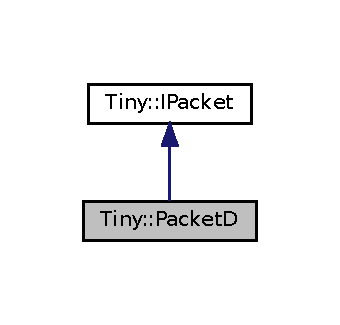
\includegraphics[width=163pt]{classTiny_1_1PacketD__inherit__graph}
\end{center}
\end{figure}


Collaboration diagram for Tiny\+:\+:PacketD\+:\nopagebreak
\begin{figure}[H]
\begin{center}
\leavevmode
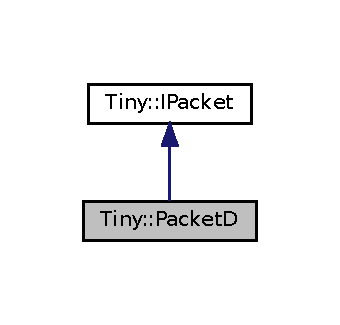
\includegraphics[width=163pt]{classTiny_1_1PacketD__coll__graph}
\end{center}
\end{figure}
\subsection*{Public Member Functions}
\begin{DoxyCompactItemize}
\item 
\hyperlink{classTiny_1_1PacketD_a337a74c5e513be616aff0c1a0746612a}{PacketD} (int \hyperlink{classTiny_1_1IPacket_a76b6389f0d47b67c8428c58c2b09df51}{size})
\end{DoxyCompactItemize}


\subsection{Detailed Description}
Class which allocated buffer for packet dynamically. Use this class only on powerful microcontrollers. 

\subsection{Constructor \& Destructor Documentation}
\mbox{\Hypertarget{classTiny_1_1PacketD_a337a74c5e513be616aff0c1a0746612a}\label{classTiny_1_1PacketD_a337a74c5e513be616aff0c1a0746612a}} 
\index{Tiny\+::\+PacketD@{Tiny\+::\+PacketD}!PacketD@{PacketD}}
\index{PacketD@{PacketD}!Tiny\+::\+PacketD@{Tiny\+::\+PacketD}}
\subsubsection{\texorpdfstring{Packet\+D()}{PacketD()}}
{\footnotesize\ttfamily Tiny\+::\+Packet\+D\+::\+PacketD (\begin{DoxyParamCaption}\item[{int}]{size }\end{DoxyParamCaption})\hspace{0.3cm}{\ttfamily [inline]}}

Creates packet with dynamically allocated buffer. 
\begin{DoxyParams}{Parameters}
{\em size} & number of bytes to allocate for the packet buffer. \\
\hline
\end{DoxyParams}


The documentation for this class was generated from the following file\+:\begin{DoxyCompactItemize}
\item 
src/\hyperlink{TinyPacket_8h}{Tiny\+Packet.\+h}\end{DoxyCompactItemize}

\hypertarget{classTiny_1_1ProtoFd}{}\section{Tiny\+:\+:Proto\+Fd$<$ S $>$ Class Template Reference}
\label{classTiny_1_1ProtoFd}\index{Tiny\+::\+Proto\+Fd$<$ S $>$@{Tiny\+::\+Proto\+Fd$<$ S $>$}}


{\ttfamily \#include $<$Tiny\+Protocol\+Fd.\+h$>$}



Inheritance diagram for Tiny\+:\+:Proto\+Fd$<$ S $>$\+:
\nopagebreak
\begin{figure}[H]
\begin{center}
\leavevmode
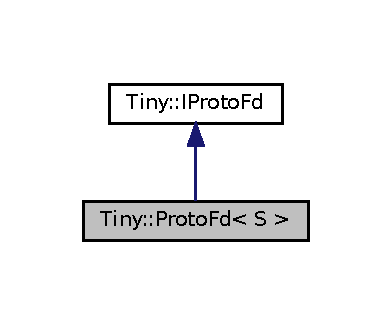
\includegraphics[width=181pt]{classTiny_1_1ProtoFd__inherit__graph}
\end{center}
\end{figure}


Collaboration diagram for Tiny\+:\+:Proto\+Fd$<$ S $>$\+:
\nopagebreak
\begin{figure}[H]
\begin{center}
\leavevmode
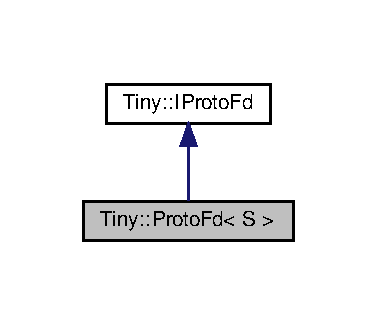
\includegraphics[width=181pt]{classTiny_1_1ProtoFd__coll__graph}
\end{center}
\end{figure}
\subsection*{Additional Inherited Members}


\subsection{Detailed Description}
\subsubsection*{template$<$int S$>$\newline
class Tiny\+::\+Proto\+Fd$<$ S $>$}

This is class, which allocates buffers statically. Use it for systems with low resources. 

The documentation for this class was generated from the following file\+:\begin{DoxyCompactItemize}
\item 
src/\hyperlink{TinyProtocolFd_8h}{Tiny\+Protocol\+Fd.\+h}\end{DoxyCompactItemize}

\hypertarget{classTiny_1_1ProtoFdD}{}\section{Tiny\+:\+:Proto\+FdD Class Reference}
\label{classTiny_1_1ProtoFdD}\index{Tiny\+::\+Proto\+FdD@{Tiny\+::\+Proto\+FdD}}


{\ttfamily \#include $<$Tiny\+Protocol\+Fd.\+h$>$}



Inheritance diagram for Tiny\+:\+:Proto\+FdD\+:
\nopagebreak
\begin{figure}[H]
\begin{center}
\leavevmode
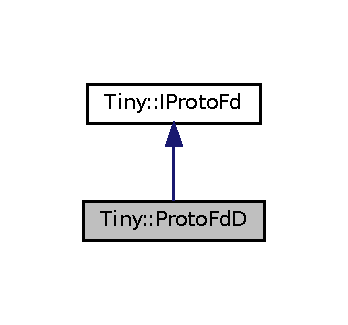
\includegraphics[width=167pt]{classTiny_1_1ProtoFdD__inherit__graph}
\end{center}
\end{figure}


Collaboration diagram for Tiny\+:\+:Proto\+FdD\+:
\nopagebreak
\begin{figure}[H]
\begin{center}
\leavevmode
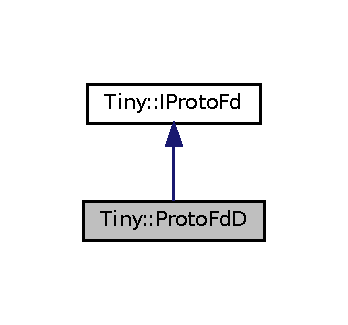
\includegraphics[width=167pt]{classTiny_1_1ProtoFdD__coll__graph}
\end{center}
\end{figure}
\subsection*{Public Member Functions}
\begin{DoxyCompactItemize}
\item 
\hyperlink{classTiny_1_1ProtoFdD_ac6d3b1143cb0776b9ae16e57068f03dc}{Proto\+FdD} (int size)
\end{DoxyCompactItemize}
\subsection*{Additional Inherited Members}


\subsection{Detailed Description}
This is special class for Full duplex protocol, which allocates buffers dynamically. We need to have separate class for this, as on small microcontrollers dynamic allocation in basic class increases flash consumption, even if dynamic memory is not used. 

\subsection{Constructor \& Destructor Documentation}
\mbox{\Hypertarget{classTiny_1_1ProtoFdD_ac6d3b1143cb0776b9ae16e57068f03dc}\label{classTiny_1_1ProtoFdD_ac6d3b1143cb0776b9ae16e57068f03dc}} 
\index{Tiny\+::\+Proto\+FdD@{Tiny\+::\+Proto\+FdD}!Proto\+FdD@{Proto\+FdD}}
\index{Proto\+FdD@{Proto\+FdD}!Tiny\+::\+Proto\+FdD@{Tiny\+::\+Proto\+FdD}}
\subsubsection{\texorpdfstring{Proto\+Fd\+D()}{ProtoFdD()}}
{\footnotesize\ttfamily Tiny\+::\+Proto\+Fd\+D\+::\+Proto\+FdD (\begin{DoxyParamCaption}\item[{int}]{size }\end{DoxyParamCaption})\hspace{0.3cm}{\ttfamily [inline]}}

Creates instance of Full duplex protocol with dynamically allocated buffer. Use this class only on powerful microcontrollers. 

The documentation for this class was generated from the following file\+:\begin{DoxyCompactItemize}
\item 
src/\hyperlink{TinyProtocolFd_8h}{Tiny\+Protocol\+Fd.\+h}\end{DoxyCompactItemize}

\hypertarget{classTiny_1_1ProtoHd}{}\section{Tiny\+:\+:Proto\+Hd Class Reference}
\label{classTiny_1_1ProtoHd}\index{Tiny\+::\+Proto\+Hd@{Tiny\+::\+Proto\+Hd}}


{\ttfamily \#include $<$Tiny\+Protocol\+Hd.\+h$>$}

\subsection*{Public Member Functions}
\begin{DoxyCompactItemize}
\item 
\hyperlink{classTiny_1_1ProtoHd_a1a55191980c259f2c760997d9c07cb48}{Proto\+Hd} (void $\ast$buffer, int buffer\+Size, void($\ast$on\+Receive)(uint8\+\_\+t $\ast$buf, int len))
\item 
void \hyperlink{classTiny_1_1ProtoHd_a112ae02531837a852af7ca3c9a32a7eb}{begin} (\hyperlink{tiny__proto__types_8h_a7f69e669de5baa69a43ee5cb439a7496}{write\+\_\+block\+\_\+cb\+\_\+t} writecb, \hyperlink{tiny__proto__types_8h_ae3d867e030f59de94508902f2b84a7ec}{read\+\_\+block\+\_\+cb\+\_\+t} readcb)
\item 
void \hyperlink{classTiny_1_1ProtoHd_a0e88ac5b3c67ca67c566742c22180050}{begin\+To\+Serial} ()
\item 
void \hyperlink{classTiny_1_1ProtoHd_a1b2975217b0523c3de4b534644cfa501}{begin\+To\+Serial1} ()
\item 
void \hyperlink{classTiny_1_1ProtoHd_a450fc792e515ffd150072988bc632c9e}{begin\+To\+Serial2} ()
\item 
void \hyperlink{classTiny_1_1ProtoHd_acd6519f6652c279b3a3b98aabbaeed65}{begin\+To\+Serial3} ()
\item 
void \hyperlink{classTiny_1_1ProtoHd_ac87bf8264895b654025001a0e6014f3f}{end} ()
\item 
int \hyperlink{classTiny_1_1ProtoHd_af53c8817317d3a62535e68ca236a038f}{write} (char $\ast$buf, int size)
\item 
int \hyperlink{classTiny_1_1ProtoHd_abffb26e95006c4e09e79f27f6ec4cdfe}{write} (\hyperlink{classTiny_1_1Packet}{Packet} \&pkt)
\item 
int \hyperlink{classTiny_1_1ProtoHd_af07b1f5d0df3021e00a4b4f04af4150b}{run} ()
\item 
void \hyperlink{classTiny_1_1ProtoHd_ae90a0a40de0b71a015f7f7f940440fa0}{disable\+Crc} ()
\item 
bool \hyperlink{classTiny_1_1ProtoHd_ace4e6b993532b3eb47d025b8db94192d}{enable\+Check\+Sum} ()
\item 
bool \hyperlink{classTiny_1_1ProtoHd_a0887adedc93b7538dbaef3fc8e0b2819}{enable\+Crc16} ()
\item 
bool \hyperlink{classTiny_1_1ProtoHd_a4110a0112548d5e47d312d190930ad20}{enable\+Crc32} ()
\end{DoxyCompactItemize}


\subsection{Detailed Description}
\hyperlink{classTiny_1_1ProtoHd}{Proto\+Hd} class incapsulates Half Duplex Protocol functionality. Half Duplex version of the Protocol allows to send messages with confirmation. Remember that you may use always C-\/style A\+PI functions instead C++. Please refer to documentation. 

\subsection{Constructor \& Destructor Documentation}
\mbox{\Hypertarget{classTiny_1_1ProtoHd_a1a55191980c259f2c760997d9c07cb48}\label{classTiny_1_1ProtoHd_a1a55191980c259f2c760997d9c07cb48}} 
\index{Tiny\+::\+Proto\+Hd@{Tiny\+::\+Proto\+Hd}!Proto\+Hd@{Proto\+Hd}}
\index{Proto\+Hd@{Proto\+Hd}!Tiny\+::\+Proto\+Hd@{Tiny\+::\+Proto\+Hd}}
\subsubsection{\texorpdfstring{Proto\+Hd()}{ProtoHd()}}
{\footnotesize\ttfamily Tiny\+::\+Proto\+Hd\+::\+Proto\+Hd (\begin{DoxyParamCaption}\item[{void $\ast$}]{buffer,  }\item[{int}]{buffer\+Size,  }\item[{void($\ast$)(uint8\+\_\+t $\ast$buf, int len)}]{on\+Receive }\end{DoxyParamCaption})\hspace{0.3cm}{\ttfamily [inline]}}

Initializes \hyperlink{classTiny_1_1ProtoHd}{Proto\+Hd} object 
\begin{DoxyParams}{Parameters}
{\em buffer} & -\/ buffer to store the frames being received. \\
\hline
{\em buffer\+Size} & -\/ size of the buffer \\
\hline
{\em on\+Receive} & -\/ callback to call when the frame is received completely. \\
\hline
\end{DoxyParams}


\subsection{Member Function Documentation}
\mbox{\Hypertarget{classTiny_1_1ProtoHd_a112ae02531837a852af7ca3c9a32a7eb}\label{classTiny_1_1ProtoHd_a112ae02531837a852af7ca3c9a32a7eb}} 
\index{Tiny\+::\+Proto\+Hd@{Tiny\+::\+Proto\+Hd}!begin@{begin}}
\index{begin@{begin}!Tiny\+::\+Proto\+Hd@{Tiny\+::\+Proto\+Hd}}
\subsubsection{\texorpdfstring{begin()}{begin()}}
{\footnotesize\ttfamily void Tiny\+::\+Proto\+Hd\+::begin (\begin{DoxyParamCaption}\item[{\hyperlink{tiny__proto__types_8h_a7f69e669de5baa69a43ee5cb439a7496}{write\+\_\+block\+\_\+cb\+\_\+t}}]{writecb,  }\item[{\hyperlink{tiny__proto__types_8h_ae3d867e030f59de94508902f2b84a7ec}{read\+\_\+block\+\_\+cb\+\_\+t}}]{readcb }\end{DoxyParamCaption})}

Initializes protocol internal variables. If you need to switch communication with other destination point, you can call this method one again after calling \hyperlink{classTiny_1_1ProtoHd_ac87bf8264895b654025001a0e6014f3f}{end()}. 
\begin{DoxyParams}{Parameters}
{\em writecb} & -\/ write function to some physical channel \\
\hline
{\em readcb} & -\/ read function from some physical channel \\
\hline
\end{DoxyParams}
\begin{DoxyReturn}{Returns}
None 
\end{DoxyReturn}
\mbox{\Hypertarget{classTiny_1_1ProtoHd_a0e88ac5b3c67ca67c566742c22180050}\label{classTiny_1_1ProtoHd_a0e88ac5b3c67ca67c566742c22180050}} 
\index{Tiny\+::\+Proto\+Hd@{Tiny\+::\+Proto\+Hd}!begin\+To\+Serial@{begin\+To\+Serial}}
\index{begin\+To\+Serial@{begin\+To\+Serial}!Tiny\+::\+Proto\+Hd@{Tiny\+::\+Proto\+Hd}}
\subsubsection{\texorpdfstring{begin\+To\+Serial()}{beginToSerial()}}
{\footnotesize\ttfamily void Tiny\+::\+Proto\+Hd\+::begin\+To\+Serial (\begin{DoxyParamCaption}{ }\end{DoxyParamCaption})\hspace{0.3cm}{\ttfamily [inline]}}

Initializes protocol internal variables and redirects communication through Arduino Serial connection (Serial). \begin{DoxyReturn}{Returns}
None 
\end{DoxyReturn}
\mbox{\Hypertarget{classTiny_1_1ProtoHd_a1b2975217b0523c3de4b534644cfa501}\label{classTiny_1_1ProtoHd_a1b2975217b0523c3de4b534644cfa501}} 
\index{Tiny\+::\+Proto\+Hd@{Tiny\+::\+Proto\+Hd}!begin\+To\+Serial1@{begin\+To\+Serial1}}
\index{begin\+To\+Serial1@{begin\+To\+Serial1}!Tiny\+::\+Proto\+Hd@{Tiny\+::\+Proto\+Hd}}
\subsubsection{\texorpdfstring{begin\+To\+Serial1()}{beginToSerial1()}}
{\footnotesize\ttfamily void Tiny\+::\+Proto\+Hd\+::begin\+To\+Serial1 (\begin{DoxyParamCaption}{ }\end{DoxyParamCaption})\hspace{0.3cm}{\ttfamily [inline]}}

Initializes protocol internal variables and redirects communication through Arduino Serial1 connection (Serial1). \begin{DoxyReturn}{Returns}
None 
\end{DoxyReturn}
\mbox{\Hypertarget{classTiny_1_1ProtoHd_a450fc792e515ffd150072988bc632c9e}\label{classTiny_1_1ProtoHd_a450fc792e515ffd150072988bc632c9e}} 
\index{Tiny\+::\+Proto\+Hd@{Tiny\+::\+Proto\+Hd}!begin\+To\+Serial2@{begin\+To\+Serial2}}
\index{begin\+To\+Serial2@{begin\+To\+Serial2}!Tiny\+::\+Proto\+Hd@{Tiny\+::\+Proto\+Hd}}
\subsubsection{\texorpdfstring{begin\+To\+Serial2()}{beginToSerial2()}}
{\footnotesize\ttfamily void Tiny\+::\+Proto\+Hd\+::begin\+To\+Serial2 (\begin{DoxyParamCaption}{ }\end{DoxyParamCaption})\hspace{0.3cm}{\ttfamily [inline]}}

Initializes protocol internal variables and redirects communication through Arduino Serial2 connection (Serial2). \begin{DoxyReturn}{Returns}
None 
\end{DoxyReturn}
\mbox{\Hypertarget{classTiny_1_1ProtoHd_acd6519f6652c279b3a3b98aabbaeed65}\label{classTiny_1_1ProtoHd_acd6519f6652c279b3a3b98aabbaeed65}} 
\index{Tiny\+::\+Proto\+Hd@{Tiny\+::\+Proto\+Hd}!begin\+To\+Serial3@{begin\+To\+Serial3}}
\index{begin\+To\+Serial3@{begin\+To\+Serial3}!Tiny\+::\+Proto\+Hd@{Tiny\+::\+Proto\+Hd}}
\subsubsection{\texorpdfstring{begin\+To\+Serial3()}{beginToSerial3()}}
{\footnotesize\ttfamily void Tiny\+::\+Proto\+Hd\+::begin\+To\+Serial3 (\begin{DoxyParamCaption}{ }\end{DoxyParamCaption})\hspace{0.3cm}{\ttfamily [inline]}}

Initializes protocol internal variables and redirects communication through Arduino Serial3 connection (Serial3). \begin{DoxyReturn}{Returns}
None 
\end{DoxyReturn}
\mbox{\Hypertarget{classTiny_1_1ProtoHd_ae90a0a40de0b71a015f7f7f940440fa0}\label{classTiny_1_1ProtoHd_ae90a0a40de0b71a015f7f7f940440fa0}} 
\index{Tiny\+::\+Proto\+Hd@{Tiny\+::\+Proto\+Hd}!disable\+Crc@{disable\+Crc}}
\index{disable\+Crc@{disable\+Crc}!Tiny\+::\+Proto\+Hd@{Tiny\+::\+Proto\+Hd}}
\subsubsection{\texorpdfstring{disable\+Crc()}{disableCrc()}}
{\footnotesize\ttfamily void Tiny\+::\+Proto\+Hd\+::disable\+Crc (\begin{DoxyParamCaption}{ }\end{DoxyParamCaption})}

Disable C\+RC field in the protocol. If C\+RC field is O\+FF, then the frame looks like this\+: 0x7E databytes 0x7E. \mbox{\Hypertarget{classTiny_1_1ProtoHd_ace4e6b993532b3eb47d025b8db94192d}\label{classTiny_1_1ProtoHd_ace4e6b993532b3eb47d025b8db94192d}} 
\index{Tiny\+::\+Proto\+Hd@{Tiny\+::\+Proto\+Hd}!enable\+Check\+Sum@{enable\+Check\+Sum}}
\index{enable\+Check\+Sum@{enable\+Check\+Sum}!Tiny\+::\+Proto\+Hd@{Tiny\+::\+Proto\+Hd}}
\subsubsection{\texorpdfstring{enable\+Check\+Sum()}{enableCheckSum()}}
{\footnotesize\ttfamily bool Tiny\+::\+Proto\+Hd\+::enable\+Check\+Sum (\begin{DoxyParamCaption}{ }\end{DoxyParamCaption})}

Enables C\+RC 8-\/bit field in the protocol. This field contains sum of all data bytes in the packet. 8-\/bit field is supported by Nano version of Tiny library. \begin{DoxyReturn}{Returns}
true if successful false in case of error. 
\end{DoxyReturn}
\mbox{\Hypertarget{classTiny_1_1ProtoHd_a0887adedc93b7538dbaef3fc8e0b2819}\label{classTiny_1_1ProtoHd_a0887adedc93b7538dbaef3fc8e0b2819}} 
\index{Tiny\+::\+Proto\+Hd@{Tiny\+::\+Proto\+Hd}!enable\+Crc16@{enable\+Crc16}}
\index{enable\+Crc16@{enable\+Crc16}!Tiny\+::\+Proto\+Hd@{Tiny\+::\+Proto\+Hd}}
\subsubsection{\texorpdfstring{enable\+Crc16()}{enableCrc16()}}
{\footnotesize\ttfamily bool Tiny\+::\+Proto\+Hd\+::enable\+Crc16 (\begin{DoxyParamCaption}{ }\end{DoxyParamCaption})}

Enables C\+RC 16-\/bit field in the protocol. This field contains F\+CS 16-\/bit C\+C\+I\+TT like defined in R\+FC 1662. 16-\/bit field is not supported by Nano version of Tiny library. \begin{DoxyReturn}{Returns}
true if successful false in case of error. 
\end{DoxyReturn}
\mbox{\Hypertarget{classTiny_1_1ProtoHd_a4110a0112548d5e47d312d190930ad20}\label{classTiny_1_1ProtoHd_a4110a0112548d5e47d312d190930ad20}} 
\index{Tiny\+::\+Proto\+Hd@{Tiny\+::\+Proto\+Hd}!enable\+Crc32@{enable\+Crc32}}
\index{enable\+Crc32@{enable\+Crc32}!Tiny\+::\+Proto\+Hd@{Tiny\+::\+Proto\+Hd}}
\subsubsection{\texorpdfstring{enable\+Crc32()}{enableCrc32()}}
{\footnotesize\ttfamily bool Tiny\+::\+Proto\+Hd\+::enable\+Crc32 (\begin{DoxyParamCaption}{ }\end{DoxyParamCaption})}

Enables C\+RC 32-\/bit field in the protocol. This field contains F\+CS 32-\/bit C\+C\+I\+TT like defined in R\+FC 1662. 32-\/bit field is not supported by Nano version of Tiny library. \begin{DoxyReturn}{Returns}
true if successful false in case of error. 
\end{DoxyReturn}
\mbox{\Hypertarget{classTiny_1_1ProtoHd_ac87bf8264895b654025001a0e6014f3f}\label{classTiny_1_1ProtoHd_ac87bf8264895b654025001a0e6014f3f}} 
\index{Tiny\+::\+Proto\+Hd@{Tiny\+::\+Proto\+Hd}!end@{end}}
\index{end@{end}!Tiny\+::\+Proto\+Hd@{Tiny\+::\+Proto\+Hd}}
\subsubsection{\texorpdfstring{end()}{end()}}
{\footnotesize\ttfamily void Tiny\+::\+Proto\+Hd\+::end (\begin{DoxyParamCaption}{ }\end{DoxyParamCaption})}

Resets protocol state. \mbox{\Hypertarget{classTiny_1_1ProtoHd_af07b1f5d0df3021e00a4b4f04af4150b}\label{classTiny_1_1ProtoHd_af07b1f5d0df3021e00a4b4f04af4150b}} 
\index{Tiny\+::\+Proto\+Hd@{Tiny\+::\+Proto\+Hd}!run@{run}}
\index{run@{run}!Tiny\+::\+Proto\+Hd@{Tiny\+::\+Proto\+Hd}}
\subsubsection{\texorpdfstring{run()}{run()}}
{\footnotesize\ttfamily int Tiny\+::\+Proto\+Hd\+::run (\begin{DoxyParamCaption}{ }\end{DoxyParamCaption})}

Checks communcation channel for incoming messages. \begin{DoxyReturn}{Returns}
negative value in case of error zero if nothing is read positive -\/ \hyperlink{classTiny_1_1Packet}{Packet} is successfully received 
\end{DoxyReturn}
\begin{DoxyRemark}{Remarks}
if \hyperlink{classTiny_1_1Packet}{Packet} is receive during run execution callback is called. 
\end{DoxyRemark}
\mbox{\Hypertarget{classTiny_1_1ProtoHd_af53c8817317d3a62535e68ca236a038f}\label{classTiny_1_1ProtoHd_af53c8817317d3a62535e68ca236a038f}} 
\index{Tiny\+::\+Proto\+Hd@{Tiny\+::\+Proto\+Hd}!write@{write}}
\index{write@{write}!Tiny\+::\+Proto\+Hd@{Tiny\+::\+Proto\+Hd}}
\subsubsection{\texorpdfstring{write()}{write()}\hspace{0.1cm}{\footnotesize\ttfamily [1/2]}}
{\footnotesize\ttfamily int Tiny\+::\+Proto\+Hd\+::write (\begin{DoxyParamCaption}\item[{char $\ast$}]{buf,  }\item[{int}]{size }\end{DoxyParamCaption})}

Sends data block over communication channel. 
\begin{DoxyParams}{Parameters}
{\em buf} & -\/ data to send \\
\hline
{\em size} & -\/ length of the data in bytes \\
\hline
\end{DoxyParams}
\begin{DoxyReturn}{Returns}
negative value in case of error zero if nothing is sent positive -\/ should be equal to size parameter 
\end{DoxyReturn}
\mbox{\Hypertarget{classTiny_1_1ProtoHd_abffb26e95006c4e09e79f27f6ec4cdfe}\label{classTiny_1_1ProtoHd_abffb26e95006c4e09e79f27f6ec4cdfe}} 
\index{Tiny\+::\+Proto\+Hd@{Tiny\+::\+Proto\+Hd}!write@{write}}
\index{write@{write}!Tiny\+::\+Proto\+Hd@{Tiny\+::\+Proto\+Hd}}
\subsubsection{\texorpdfstring{write()}{write()}\hspace{0.1cm}{\footnotesize\ttfamily [2/2]}}
{\footnotesize\ttfamily int Tiny\+::\+Proto\+Hd\+::write (\begin{DoxyParamCaption}\item[{\hyperlink{classTiny_1_1Packet}{Packet} \&}]{pkt }\end{DoxyParamCaption})}

Sends packet over communication channel. 
\begin{DoxyParams}{Parameters}
{\em pkt} & -\/ \hyperlink{classTiny_1_1Packet}{Packet} to send \\
\hline
\end{DoxyParams}
\begin{DoxySeeAlso}{See also}
\hyperlink{classTiny_1_1Packet}{Packet} 
\end{DoxySeeAlso}
\begin{DoxyReturn}{Returns}
negative value in case of error zero if nothing is sent positive -\/ \hyperlink{classTiny_1_1Packet}{Packet} is successfully sent 
\end{DoxyReturn}


The documentation for this class was generated from the following file\+:\begin{DoxyCompactItemize}
\item 
src/\hyperlink{TinyProtocolHd_8h}{Tiny\+Protocol\+Hd.\+h}\end{DoxyCompactItemize}

\hypertarget{classTiny_1_1ProtoLight}{}\section{Tiny\+:\+:Proto\+Light Class Reference}
\label{classTiny_1_1ProtoLight}\index{Tiny\+::\+Proto\+Light@{Tiny\+::\+Proto\+Light}}


{\ttfamily \#include $<$Tiny\+Light\+Protocol.\+h$>$}

\subsection*{Public Member Functions}
\begin{DoxyCompactItemize}
\item 
void \hyperlink{classTiny_1_1ProtoLight_ad27dfcef54a8316228469ef0a4267962}{begin} (write\+\_\+block\+\_\+cb\+\_\+t writecb, read\+\_\+block\+\_\+cb\+\_\+t readcb)
\item 
void \hyperlink{classTiny_1_1ProtoLight_a50bf63fe1891edda48980ca2893485d7}{begin\+To\+Serial} ()
\item 
void \hyperlink{classTiny_1_1ProtoLight_a948b2a0e37177b7434581adc64b36497}{end} ()
\item 
int \hyperlink{classTiny_1_1ProtoLight_a46a27ee9d0b55c88672c98abf04dbdce}{write} (char $\ast$buf, int size)
\item 
int \hyperlink{classTiny_1_1ProtoLight_acf18a8b73ee6c6394270c903ad7882b8}{read} (char $\ast$buf, int size)
\item 
int \hyperlink{classTiny_1_1ProtoLight_abf2966531f8ed7dba44079f00eefded2}{write} (\hyperlink{classTiny_1_1Packet}{Packet} \&pkt)
\item 
int \hyperlink{classTiny_1_1ProtoLight_a96c56b10b4eee28c09b291461c66fa54}{read} (\hyperlink{classTiny_1_1Packet}{Packet} \&pkt)
\end{DoxyCompactItemize}


\subsection{Detailed Description}
\hyperlink{classTiny_1_1ProtoLight}{Proto\+Light} class incapsulates Protocol functionality. Remember that you may use always C-\/style A\+P\+I functions instead C++. Please refer to documentation. 

\subsection{Member Function Documentation}
\hypertarget{classTiny_1_1ProtoLight_ad27dfcef54a8316228469ef0a4267962}{}\index{Tiny\+::\+Proto\+Light@{Tiny\+::\+Proto\+Light}!begin@{begin}}
\index{begin@{begin}!Tiny\+::\+Proto\+Light@{Tiny\+::\+Proto\+Light}}
\subsubsection[{begin}]{\setlength{\rightskip}{0pt plus 5cm}void Tiny\+::\+Proto\+Light\+::begin (
\begin{DoxyParamCaption}
\item[{write\+\_\+block\+\_\+cb\+\_\+t}]{writecb, }
\item[{read\+\_\+block\+\_\+cb\+\_\+t}]{readcb}
\end{DoxyParamCaption}
)}\label{classTiny_1_1ProtoLight_ad27dfcef54a8316228469ef0a4267962}
Initializes protocol internal variables. If you need to switch communication with other destination point, you can call this method one again after calling \hyperlink{classTiny_1_1ProtoLight_a948b2a0e37177b7434581adc64b36497}{end()}. 
\begin{DoxyParams}{Parameters}
{\em writecb} & -\/ write function to some physical channel \\
\hline
{\em readcb} & -\/ read function from some physical channel \\
\hline
\end{DoxyParams}
\begin{DoxyReturn}{Returns}
None 
\end{DoxyReturn}
\hypertarget{classTiny_1_1ProtoLight_a50bf63fe1891edda48980ca2893485d7}{}\index{Tiny\+::\+Proto\+Light@{Tiny\+::\+Proto\+Light}!begin\+To\+Serial@{begin\+To\+Serial}}
\index{begin\+To\+Serial@{begin\+To\+Serial}!Tiny\+::\+Proto\+Light@{Tiny\+::\+Proto\+Light}}
\subsubsection[{begin\+To\+Serial}]{\setlength{\rightskip}{0pt plus 5cm}void Tiny\+::\+Proto\+Light\+::begin\+To\+Serial (
\begin{DoxyParamCaption}
{}
\end{DoxyParamCaption}
)}\label{classTiny_1_1ProtoLight_a50bf63fe1891edda48980ca2893485d7}
Initializes protocol internal variables and redirects communication through Arduino Serial connection (Serial). \begin{DoxyReturn}{Returns}
None 
\end{DoxyReturn}
\hypertarget{classTiny_1_1ProtoLight_a948b2a0e37177b7434581adc64b36497}{}\index{Tiny\+::\+Proto\+Light@{Tiny\+::\+Proto\+Light}!end@{end}}
\index{end@{end}!Tiny\+::\+Proto\+Light@{Tiny\+::\+Proto\+Light}}
\subsubsection[{end}]{\setlength{\rightskip}{0pt plus 5cm}void Tiny\+::\+Proto\+Light\+::end (
\begin{DoxyParamCaption}
{}
\end{DoxyParamCaption}
)}\label{classTiny_1_1ProtoLight_a948b2a0e37177b7434581adc64b36497}
Resets protocol state. \hypertarget{classTiny_1_1ProtoLight_acf18a8b73ee6c6394270c903ad7882b8}{}\index{Tiny\+::\+Proto\+Light@{Tiny\+::\+Proto\+Light}!read@{read}}
\index{read@{read}!Tiny\+::\+Proto\+Light@{Tiny\+::\+Proto\+Light}}
\subsubsection[{read}]{\setlength{\rightskip}{0pt plus 5cm}int Tiny\+::\+Proto\+Light\+::read (
\begin{DoxyParamCaption}
\item[{char $\ast$}]{buf, }
\item[{int}]{size}
\end{DoxyParamCaption}
)}\label{classTiny_1_1ProtoLight_acf18a8b73ee6c6394270c903ad7882b8}
Reads data block from communication channel. 
\begin{DoxyParams}{Parameters}
{\em buf} & -\/ buffer to place data read from communication channel \\
\hline
{\em size} & -\/ maximum size of the buffer in bytes. \\
\hline
\end{DoxyParams}
\begin{DoxyReturn}{Returns}
negative value in case of error zero if nothing is read positive -\/ number of bytes read from the channel 
\end{DoxyReturn}
\hypertarget{classTiny_1_1ProtoLight_a96c56b10b4eee28c09b291461c66fa54}{}\index{Tiny\+::\+Proto\+Light@{Tiny\+::\+Proto\+Light}!read@{read}}
\index{read@{read}!Tiny\+::\+Proto\+Light@{Tiny\+::\+Proto\+Light}}
\subsubsection[{read}]{\setlength{\rightskip}{0pt plus 5cm}int Tiny\+::\+Proto\+Light\+::read (
\begin{DoxyParamCaption}
\item[{{\bf Packet} \&}]{pkt}
\end{DoxyParamCaption}
)}\label{classTiny_1_1ProtoLight_a96c56b10b4eee28c09b291461c66fa54}
Reads packet from communication channel. 
\begin{DoxyParams}{Parameters}
{\em pkt} & -\/ \hyperlink{classTiny_1_1Packet}{Packet} object to put data to \\
\hline
\end{DoxyParams}
\begin{DoxySeeAlso}{See also}
\hyperlink{classTiny_1_1Packet}{Packet} 
\end{DoxySeeAlso}
\begin{DoxyReturn}{Returns}
negative value in case of error zero if nothing is read positive -\/ \hyperlink{classTiny_1_1Packet}{Packet} is successfully received 
\end{DoxyReturn}
\hypertarget{classTiny_1_1ProtoLight_a46a27ee9d0b55c88672c98abf04dbdce}{}\index{Tiny\+::\+Proto\+Light@{Tiny\+::\+Proto\+Light}!write@{write}}
\index{write@{write}!Tiny\+::\+Proto\+Light@{Tiny\+::\+Proto\+Light}}
\subsubsection[{write}]{\setlength{\rightskip}{0pt plus 5cm}int Tiny\+::\+Proto\+Light\+::write (
\begin{DoxyParamCaption}
\item[{char $\ast$}]{buf, }
\item[{int}]{size}
\end{DoxyParamCaption}
)}\label{classTiny_1_1ProtoLight_a46a27ee9d0b55c88672c98abf04dbdce}
Sends data block over communication channel. 
\begin{DoxyParams}{Parameters}
{\em buf} & -\/ data to send \\
\hline
{\em size} & -\/ length of the data in bytes \\
\hline
\end{DoxyParams}
\begin{DoxyReturn}{Returns}
negative value in case of error zero if nothing is sent positive -\/ should be equal to size parameter 
\end{DoxyReturn}
\hypertarget{classTiny_1_1ProtoLight_abf2966531f8ed7dba44079f00eefded2}{}\index{Tiny\+::\+Proto\+Light@{Tiny\+::\+Proto\+Light}!write@{write}}
\index{write@{write}!Tiny\+::\+Proto\+Light@{Tiny\+::\+Proto\+Light}}
\subsubsection[{write}]{\setlength{\rightskip}{0pt plus 5cm}int Tiny\+::\+Proto\+Light\+::write (
\begin{DoxyParamCaption}
\item[{{\bf Packet} \&}]{pkt}
\end{DoxyParamCaption}
)}\label{classTiny_1_1ProtoLight_abf2966531f8ed7dba44079f00eefded2}
Sends packet over communication channel. 
\begin{DoxyParams}{Parameters}
{\em pkt} & -\/ \hyperlink{classTiny_1_1Packet}{Packet} to send \\
\hline
\end{DoxyParams}
\begin{DoxySeeAlso}{See also}
\hyperlink{classTiny_1_1Packet}{Packet} 
\end{DoxySeeAlso}
\begin{DoxyReturn}{Returns}
negative value in case of error zero if nothing is sent positive -\/ \hyperlink{classTiny_1_1Packet}{Packet} is successfully sent 
\end{DoxyReturn}


The documentation for this class was generated from the following file\+:\begin{DoxyCompactItemize}
\item 
src/arduino/src/\hyperlink{TinyLightProtocol_8h}{Tiny\+Light\+Protocol.\+h}\end{DoxyCompactItemize}

\hypertarget{structSTinyHdData__}{}\section{S\+Tiny\+Hd\+Data\+\_\+ Struct Reference}
\label{structSTinyHdData__}\index{S\+Tiny\+Hd\+Data\+\_\+@{S\+Tiny\+Hd\+Data\+\_\+}}


{\ttfamily \#include $<$tiny\+\_\+hd.\+h$>$}



Collaboration diagram for S\+Tiny\+Hd\+Data\+\_\+\+:
\nopagebreak
\begin{figure}[H]
\begin{center}
\leavevmode
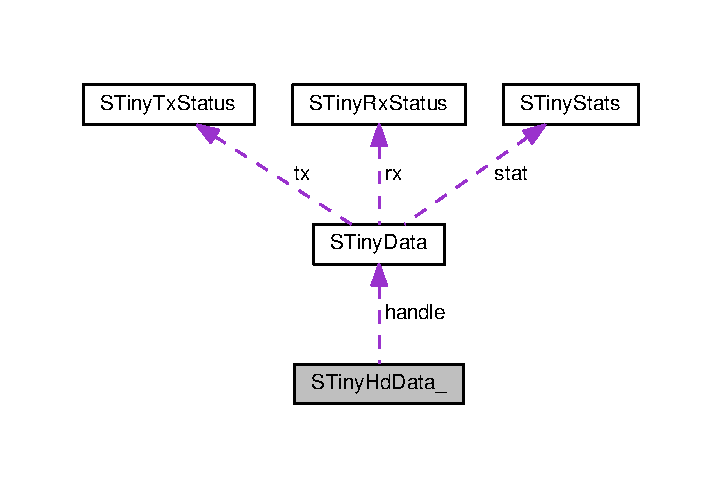
\includegraphics[width=263pt]{structSTinyHdData____coll__graph}
\end{center}
\end{figure}
\subsection*{Public Attributes}
\begin{DoxyCompactItemize}
\item 
\hypertarget{structSTinyHdData___a0df5a323cbbfd49fb138b14bca73f14c}{}\hyperlink{structSTinyData}{S\+Tiny\+Data} \hyperlink{structSTinyHdData___a0df5a323cbbfd49fb138b14bca73f14c}{handle}\label{structSTinyHdData___a0df5a323cbbfd49fb138b14bca73f14c}

\begin{DoxyCompactList}\small\item\em Original \hyperlink{structSTinyData}{S\+Tiny\+Data} structure. It is used to control lower level. \end{DoxyCompactList}\item 
\hypertarget{structSTinyHdData___abf8a0eb5006769a92adc186554a3a1c0}{}on\+\_\+frame\+\_\+cb\+\_\+t \hyperlink{structSTinyHdData___abf8a0eb5006769a92adc186554a3a1c0}{on\+\_\+frame\+\_\+cb}\label{structSTinyHdData___abf8a0eb5006769a92adc186554a3a1c0}

\begin{DoxyCompactList}\small\item\em Callback to process received frames. \end{DoxyCompactList}\item 
\hypertarget{structSTinyHdData___a69a6bb34b580bcfa5e13112cb7652d1d}{}void $\ast$ \hyperlink{structSTinyHdData___a69a6bb34b580bcfa5e13112cb7652d1d}{inbuf}\label{structSTinyHdData___a69a6bb34b580bcfa5e13112cb7652d1d}

\begin{DoxyCompactList}\small\item\em Buffer to store frames being received. \end{DoxyCompactList}\item 
\hypertarget{structSTinyHdData___adbad190a4b54eccd4da6f3c3305a54f1}{}uint16\+\_\+t \hyperlink{structSTinyHdData___adbad190a4b54eccd4da6f3c3305a54f1}{inbuf\+\_\+size}\label{structSTinyHdData___adbad190a4b54eccd4da6f3c3305a54f1}

\begin{DoxyCompactList}\small\item\em maximum size of Rx buffer \end{DoxyCompactList}\item 
\hypertarget{structSTinyHdData___a7ca4e5b23cf480d93317245010bcbe73}{}uint16\+\_\+t \hyperlink{structSTinyHdData___a7ca4e5b23cf480d93317245010bcbe73}{timeout}\label{structSTinyHdData___a7ca4e5b23cf480d93317245010bcbe73}

\begin{DoxyCompactList}\small\item\em Timeout for operations with acknowledge. \end{DoxyCompactList}\item 
\hypertarget{structSTinyHdData___a7084eac08b744ad0aa2624b854866825}{}uint16\+\_\+t \hyperlink{structSTinyHdData___a7084eac08b744ad0aa2624b854866825}{uid}\label{structSTinyHdData___a7084eac08b744ad0aa2624b854866825}

\begin{DoxyCompactList}\small\item\em field used to store temporary uid \end{DoxyCompactList}\item 
\hypertarget{structSTinyHdData___a37dca10adb0dd210f02365b7fa20a598}{}uint8\+\_\+t \hyperlink{structSTinyHdData___a37dca10adb0dd210f02365b7fa20a598}{multithread\+\_\+mode}\label{structSTinyHdData___a37dca10adb0dd210f02365b7fa20a598}

\begin{DoxyCompactList}\small\item\em only single thread mode is supporte now. Should be zero \end{DoxyCompactList}\end{DoxyCompactItemize}


\subsection{Detailed Description}
This structure contains service data, required for half-\/duplex functioning. 

The documentation for this struct was generated from the following file\+:\begin{DoxyCompactItemize}
\item 
inc/\hyperlink{tiny__hd_8h}{tiny\+\_\+hd.\+h}\end{DoxyCompactItemize}

\hypertarget{structSTinyHdInit__}{}\section{S\+Tiny\+Hd\+Init\+\_\+ Struct Reference}
\label{structSTinyHdInit__}\index{S\+Tiny\+Hd\+Init\+\_\+@{S\+Tiny\+Hd\+Init\+\_\+}}


{\ttfamily \#include $<$tiny\+\_\+hd.\+h$>$}

\subsection*{Public Attributes}
\begin{DoxyCompactItemize}
\item 
\mbox{\Hypertarget{structSTinyHdInit___a0bd05a4fc43236ff37d67aec4d2a0952}\label{structSTinyHdInit___a0bd05a4fc43236ff37d67aec4d2a0952}} 
\hyperlink{tiny__proto__types_8h_a7f69e669de5baa69a43ee5cb439a7496}{write\+\_\+block\+\_\+cb\+\_\+t} \hyperlink{structSTinyHdInit___a0bd05a4fc43236ff37d67aec4d2a0952}{write\+\_\+func}
\begin{DoxyCompactList}\small\item\em callback function to write bytes to the physical channel \end{DoxyCompactList}\item 
\mbox{\Hypertarget{structSTinyHdInit___a5de352b11ca7915737bc459cde7c566d}\label{structSTinyHdInit___a5de352b11ca7915737bc459cde7c566d}} 
\hyperlink{tiny__proto__types_8h_ae3d867e030f59de94508902f2b84a7ec}{read\+\_\+block\+\_\+cb\+\_\+t} \hyperlink{structSTinyHdInit___a5de352b11ca7915737bc459cde7c566d}{read\+\_\+func}
\begin{DoxyCompactList}\small\item\em callback function to read buytes from the physical channel \end{DoxyCompactList}\item 
\mbox{\Hypertarget{structSTinyHdInit___a7b6be4e09ea04eaa4372eadce4d51055}\label{structSTinyHdInit___a7b6be4e09ea04eaa4372eadce4d51055}} 
void $\ast$ \hyperlink{structSTinyHdInit___a7b6be4e09ea04eaa4372eadce4d51055}{pdata}
\begin{DoxyCompactList}\small\item\em user data for block read/write functions \end{DoxyCompactList}\item 
\mbox{\Hypertarget{structSTinyHdInit___ae2eea5181620dfbb47b60a5073bd5ed2}\label{structSTinyHdInit___ae2eea5181620dfbb47b60a5073bd5ed2}} 
\hyperlink{tiny__proto__types_8h_ad6bf709565b8aecb9e6ecf196f219d54}{on\+\_\+frame\+\_\+cb\+\_\+t} \hyperlink{structSTinyHdInit___ae2eea5181620dfbb47b60a5073bd5ed2}{on\+\_\+frame\+\_\+cb}
\begin{DoxyCompactList}\small\item\em callback function to process incoming frames \end{DoxyCompactList}\item 
\mbox{\Hypertarget{structSTinyHdInit___a5996a48606a90ff9938e4037612cf97d}\label{structSTinyHdInit___a5996a48606a90ff9938e4037612cf97d}} 
void $\ast$ \hyperlink{structSTinyHdInit___a5996a48606a90ff9938e4037612cf97d}{inbuf}
\begin{DoxyCompactList}\small\item\em buffer to store input bytes being received. Must be at least maximum packet size over communication channel \end{DoxyCompactList}\item 
\mbox{\Hypertarget{structSTinyHdInit___a0eed47c62a16fa29435d480541989cf6}\label{structSTinyHdInit___a0eed47c62a16fa29435d480541989cf6}} 
uint16\+\_\+t \hyperlink{structSTinyHdInit___a0eed47c62a16fa29435d480541989cf6}{inbuf\+\_\+size}
\begin{DoxyCompactList}\small\item\em maximum input buffer size \end{DoxyCompactList}\item 
\mbox{\Hypertarget{structSTinyHdInit___ac7a1ae9314efc1296d78927198f07ac8}\label{structSTinyHdInit___ac7a1ae9314efc1296d78927198f07ac8}} 
uint16\+\_\+t \hyperlink{structSTinyHdInit___ac7a1ae9314efc1296d78927198f07ac8}{timeout}
\begin{DoxyCompactList}\small\item\em timeout. Can be set to 0 during initialization. In this case timeout will be set to default \end{DoxyCompactList}\item 
\mbox{\Hypertarget{structSTinyHdInit___a404947e25922fa8400daa924a032897e}\label{structSTinyHdInit___a404947e25922fa8400daa924a032897e}} 
uint8\+\_\+t \hyperlink{structSTinyHdInit___a404947e25922fa8400daa924a032897e}{multithread\+\_\+mode}
\begin{DoxyCompactList}\small\item\em multithread mode. At present should be 0 \end{DoxyCompactList}\end{DoxyCompactItemize}


\subsection{Detailed Description}
This structure is used for initialization of Tiny Half Duplex protocol. 

The documentation for this struct was generated from the following file\+:\begin{DoxyCompactItemize}
\item 
src/proto/\hyperlink{tiny__hd_8h}{tiny\+\_\+hd.\+h}\end{DoxyCompactItemize}

\hypertarget{structSTinyLightData}{}\section{S\+Tiny\+Light\+Data Struct Reference}
\label{structSTinyLightData}\index{S\+Tiny\+Light\+Data@{S\+Tiny\+Light\+Data}}


{\ttfamily \#include $<$tiny\+\_\+light.\+h$>$}



Collaboration diagram for S\+Tiny\+Light\+Data\+:\nopagebreak
\begin{figure}[H]
\begin{center}
\leavevmode
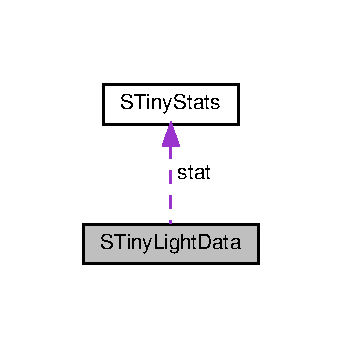
\includegraphics[width=164pt]{structSTinyLightData__coll__graph}
\end{center}
\end{figure}
\subsection*{Public Attributes}
\begin{DoxyCompactItemize}
\item 
\hyperlink{structSTinyStats}{S\+Tiny\+Stats} \hyperlink{structSTinyLightData_a623323a7a84807b5ce14a7cb56ec07f0}{stat}
\item 
\mbox{\Hypertarget{structSTinyLightData_a0bd1b1a01e1eaa15f22dec1e886c2e3c}\label{structSTinyLightData_a0bd1b1a01e1eaa15f22dec1e886c2e3c}} 
\hyperlink{tiny__proto__types_8h_aafd634660bba76cace57a8f9b01e044d}{write\+\_\+block\+\_\+cb\+\_\+t} \hyperlink{structSTinyLightData_a0bd1b1a01e1eaa15f22dec1e886c2e3c}{write\+\_\+func}
\begin{DoxyCompactList}\small\item\em pointer to platform related write function \end{DoxyCompactList}\item 
\mbox{\Hypertarget{structSTinyLightData_af9b045852adb08c137abce21d02f00ea}\label{structSTinyLightData_af9b045852adb08c137abce21d02f00ea}} 
\hyperlink{tiny__proto__types_8h_a15bec127d9ee63658563d62e92b5261b}{read\+\_\+block\+\_\+cb\+\_\+t} \hyperlink{structSTinyLightData_af9b045852adb08c137abce21d02f00ea}{read\+\_\+func}
\begin{DoxyCompactList}\small\item\em pointer to platform related read function \end{DoxyCompactList}\item 
\mbox{\Hypertarget{structSTinyLightData_a5208b2627e6bda09c3b839f4d1ad2815}\label{structSTinyLightData_a5208b2627e6bda09c3b839f4d1ad2815}} 
void $\ast$ \hyperlink{structSTinyLightData_a5208b2627e6bda09c3b839f4d1ad2815}{user\+\_\+data}
\begin{DoxyCompactList}\small\item\em user-\/specific data \end{DoxyCompactList}\end{DoxyCompactItemize}


\subsection{Detailed Description}
This structure contains information about communication channel and its state. \begin{DoxyWarning}{Warning}
This is for internal use only, and should not be accessed directly from the application. 
\end{DoxyWarning}


\subsection{Member Data Documentation}
\mbox{\Hypertarget{structSTinyLightData_a623323a7a84807b5ce14a7cb56ec07f0}\label{structSTinyLightData_a623323a7a84807b5ce14a7cb56ec07f0}} 
\index{S\+Tiny\+Light\+Data@{S\+Tiny\+Light\+Data}!stat@{stat}}
\index{stat@{stat}!S\+Tiny\+Light\+Data@{S\+Tiny\+Light\+Data}}
\subsubsection{\texorpdfstring{stat}{stat}}
{\footnotesize\ttfamily \hyperlink{structSTinyStats}{S\+Tiny\+Stats} S\+Tiny\+Light\+Data\+::stat}

\begin{DoxySeeAlso}{See also}
\hyperlink{structSTinyStats}{S\+Tiny\+Stats} 
\end{DoxySeeAlso}


The documentation for this struct was generated from the following file\+:\begin{DoxyCompactItemize}
\item 
src/proto/light/\hyperlink{tiny__light_8h}{tiny\+\_\+light.\+h}\end{DoxyCompactItemize}

\hypertarget{structSTinyStats}{}\section{S\+Tiny\+Stats Struct Reference}
\label{structSTinyStats}\index{S\+Tiny\+Stats@{S\+Tiny\+Stats}}


{\ttfamily \#include $<$tiny\+\_\+types.\+h$>$}

\subsection*{Public Attributes}
\begin{DoxyCompactItemize}
\item 
\mbox{\Hypertarget{structSTinyStats_a79119146606964d4e3345a0c019db329}\label{structSTinyStats_a79119146606964d4e3345a0c019db329}} 
uint32\+\_\+t \hyperlink{structSTinyStats_a79119146606964d4e3345a0c019db329}{oosync\+Bytes}
\begin{DoxyCompactList}\small\item\em Number of bytes received out of frame bytes. \end{DoxyCompactList}\item 
\mbox{\Hypertarget{structSTinyStats_a3ee26fa17e5afd758b4c7f2086bc0cbc}\label{structSTinyStats_a3ee26fa17e5afd758b4c7f2086bc0cbc}} 
uint32\+\_\+t \hyperlink{structSTinyStats_a3ee26fa17e5afd758b4c7f2086bc0cbc}{bytes\+Sent}
\begin{DoxyCompactList}\small\item\em Number of payload bytes totally sent through the channel. \end{DoxyCompactList}\item 
\mbox{\Hypertarget{structSTinyStats_ab58c342d0fc862c193bff6f71dc725ac}\label{structSTinyStats_ab58c342d0fc862c193bff6f71dc725ac}} 
uint32\+\_\+t \hyperlink{structSTinyStats_ab58c342d0fc862c193bff6f71dc725ac}{bytes\+Received}
\begin{DoxyCompactList}\small\item\em Number of payload bytes totally received through the channel. \end{DoxyCompactList}\item 
\mbox{\Hypertarget{structSTinyStats_a0bc110aa81a7dea0d0d64e359fb06dc3}\label{structSTinyStats_a0bc110aa81a7dea0d0d64e359fb06dc3}} 
uint32\+\_\+t \hyperlink{structSTinyStats_a0bc110aa81a7dea0d0d64e359fb06dc3}{frames\+Sent}
\begin{DoxyCompactList}\small\item\em Number of frames, successfully sent through the channel. \end{DoxyCompactList}\item 
\mbox{\Hypertarget{structSTinyStats_a19dfd3a62dbb9d86f6fb77eb1ea6f871}\label{structSTinyStats_a19dfd3a62dbb9d86f6fb77eb1ea6f871}} 
uint32\+\_\+t \hyperlink{structSTinyStats_a19dfd3a62dbb9d86f6fb77eb1ea6f871}{frames\+Received}
\begin{DoxyCompactList}\small\item\em Number of frames, successfully received through the communication channel. \end{DoxyCompactList}\item 
\mbox{\Hypertarget{structSTinyStats_abe4f4a9455b532e22f29e60789386130}\label{structSTinyStats_abe4f4a9455b532e22f29e60789386130}} 
uint32\+\_\+t \hyperlink{structSTinyStats_abe4f4a9455b532e22f29e60789386130}{frames\+Broken}
\begin{DoxyCompactList}\small\item\em Number of broken frames received. \end{DoxyCompactList}\end{DoxyCompactItemize}


\subsection{Detailed Description}
This structure contains captured statistics while the protocol sends and receives messages. 

The documentation for this struct was generated from the following file\+:\begin{DoxyCompactItemize}
\item 
src/proto/hal/\hyperlink{tiny__types_8h}{tiny\+\_\+types.\+h}\end{DoxyCompactItemize}

\hypertarget{structtiny__fd__init__t__}{}\section{tiny\+\_\+fd\+\_\+init\+\_\+t\+\_\+ Struct Reference}
\label{structtiny__fd__init__t__}\index{tiny\+\_\+fd\+\_\+init\+\_\+t\+\_\+@{tiny\+\_\+fd\+\_\+init\+\_\+t\+\_\+}}


{\ttfamily \#include $<$tiny\+\_\+fd.\+h$>$}

\subsection*{Public Attributes}
\begin{DoxyCompactItemize}
\item 
\mbox{\Hypertarget{structtiny__fd__init__t___a09606a8bdc239aeb3744a63f48585844}\label{structtiny__fd__init__t___a09606a8bdc239aeb3744a63f48585844}} 
\hyperlink{tiny__types_8h_aafd634660bba76cace57a8f9b01e044d}{write\+\_\+block\+\_\+cb\+\_\+t} \hyperlink{structtiny__fd__init__t___a09606a8bdc239aeb3744a63f48585844}{write\+\_\+func}
\begin{DoxyCompactList}\small\item\em callback function to write bytes to the physical channel \end{DoxyCompactList}\item 
\mbox{\Hypertarget{structtiny__fd__init__t___a5b241b958dbbc00dc8d5a6457ea61ed0}\label{structtiny__fd__init__t___a5b241b958dbbc00dc8d5a6457ea61ed0}} 
\hyperlink{tiny__types_8h_a15bec127d9ee63658563d62e92b5261b}{read\+\_\+block\+\_\+cb\+\_\+t} \hyperlink{structtiny__fd__init__t___a5b241b958dbbc00dc8d5a6457ea61ed0}{read\+\_\+func}
\begin{DoxyCompactList}\small\item\em callback function to read bytes from the physical channel \end{DoxyCompactList}\item 
\mbox{\Hypertarget{structtiny__fd__init__t___ac5e99328c76e8c11f98f1f9c911bde6e}\label{structtiny__fd__init__t___ac5e99328c76e8c11f98f1f9c911bde6e}} 
void $\ast$ \hyperlink{structtiny__fd__init__t___ac5e99328c76e8c11f98f1f9c911bde6e}{pdata}
\begin{DoxyCompactList}\small\item\em user data for block read/write functions \end{DoxyCompactList}\item 
\mbox{\Hypertarget{structtiny__fd__init__t___a437d94ac2f58ea83f510e0a35733f3a1}\label{structtiny__fd__init__t___a437d94ac2f58ea83f510e0a35733f3a1}} 
\hyperlink{tiny__types_8h_ad6bf709565b8aecb9e6ecf196f219d54}{on\+\_\+frame\+\_\+cb\+\_\+t} \hyperlink{structtiny__fd__init__t___a437d94ac2f58ea83f510e0a35733f3a1}{on\+\_\+frame\+\_\+cb}
\begin{DoxyCompactList}\small\item\em callback function to process incoming frames. Callback is called from \hyperlink{group__FULL__DUPLEX__API_gad31f944514aef01e27bc3ec67fdbe140}{tiny\+\_\+fd\+\_\+run\+\_\+rx()} context. \end{DoxyCompactList}\item 
\mbox{\Hypertarget{structtiny__fd__init__t___ab256903ac157e22647dc37d4aee6a986}\label{structtiny__fd__init__t___ab256903ac157e22647dc37d4aee6a986}} 
\hyperlink{tiny__types_8h_ad6bf709565b8aecb9e6ecf196f219d54}{on\+\_\+frame\+\_\+cb\+\_\+t} \hyperlink{structtiny__fd__init__t___ab256903ac157e22647dc37d4aee6a986}{on\+\_\+sent\+\_\+cb}
\begin{DoxyCompactList}\small\item\em Callback to get notification of sent frames. Callback is called from \hyperlink{group__FULL__DUPLEX__API_ga601c9874a570331580856c1ea28f7914}{tiny\+\_\+fd\+\_\+run\+\_\+tx()} context. \end{DoxyCompactList}\item 
void $\ast$ \hyperlink{structtiny__fd__init__t___a9a82b8c6c060dbc17022a0c902d436f2}{buffer}
\item 
\mbox{\Hypertarget{structtiny__fd__init__t___af76a7f851dc110e5c3f506f66ae91320}\label{structtiny__fd__init__t___af76a7f851dc110e5c3f506f66ae91320}} 
uint16\+\_\+t \hyperlink{structtiny__fd__init__t___af76a7f851dc110e5c3f506f66ae91320}{buffer\+\_\+size}
\begin{DoxyCompactList}\small\item\em maximum input buffer size, see \hyperlink{group__FULL__DUPLEX__API_ga19789bea5b5acd68804773f0d6b0e3f7}{tiny\+\_\+fd\+\_\+buffer\+\_\+size\+\_\+by\+\_\+mtu()} \end{DoxyCompactList}\item 
uint16\+\_\+t \hyperlink{structtiny__fd__init__t___ae6653af324c07711c4b20360760c3e3a}{send\+\_\+timeout}
\item 
uint16\+\_\+t \hyperlink{structtiny__fd__init__t___a54b9c689fba5aae8ccc0c29f05a159ca}{retry\+\_\+timeout}
\item 
uint8\+\_\+t \hyperlink{structtiny__fd__init__t___ae366ae6e7626b0d92a6e5088c29169cd}{retries}
\item 
\hyperlink{group__HDLC__API_gabb73b32d08d8e79eefe9385634a74bf7}{hdlc\+\_\+crc\+\_\+t} \hyperlink{structtiny__fd__init__t___ac69d819ccec020c8382eee492070a85a}{crc\+\_\+type}
\item 
uint8\+\_\+t \hyperlink{structtiny__fd__init__t___ae4da012c3e39c4e7dda587191b4c2f77}{window\+\_\+frames}
\end{DoxyCompactItemize}


\subsection{Detailed Description}
This structure is used for initialization of Tiny Full Duplex protocol. 

\subsection{Member Data Documentation}
\mbox{\Hypertarget{structtiny__fd__init__t___a9a82b8c6c060dbc17022a0c902d436f2}\label{structtiny__fd__init__t___a9a82b8c6c060dbc17022a0c902d436f2}} 
\index{tiny\+\_\+fd\+\_\+init\+\_\+t\+\_\+@{tiny\+\_\+fd\+\_\+init\+\_\+t\+\_\+}!buffer@{buffer}}
\index{buffer@{buffer}!tiny\+\_\+fd\+\_\+init\+\_\+t\+\_\+@{tiny\+\_\+fd\+\_\+init\+\_\+t\+\_\+}}
\subsubsection{\texorpdfstring{buffer}{buffer}}
{\footnotesize\ttfamily void$\ast$ tiny\+\_\+fd\+\_\+init\+\_\+t\+\_\+\+::buffer}

buffer to store data during full-\/duplex protocol operating. The size should be at least size returned by \hyperlink{group__FULL__DUPLEX__API_ga19789bea5b5acd68804773f0d6b0e3f7}{tiny\+\_\+fd\+\_\+buffer\+\_\+size\+\_\+by\+\_\+mtu()} \mbox{\Hypertarget{structtiny__fd__init__t___ac69d819ccec020c8382eee492070a85a}\label{structtiny__fd__init__t___ac69d819ccec020c8382eee492070a85a}} 
\index{tiny\+\_\+fd\+\_\+init\+\_\+t\+\_\+@{tiny\+\_\+fd\+\_\+init\+\_\+t\+\_\+}!crc\+\_\+type@{crc\+\_\+type}}
\index{crc\+\_\+type@{crc\+\_\+type}!tiny\+\_\+fd\+\_\+init\+\_\+t\+\_\+@{tiny\+\_\+fd\+\_\+init\+\_\+t\+\_\+}}
\subsubsection{\texorpdfstring{crc\+\_\+type}{crc\_type}}
{\footnotesize\ttfamily \hyperlink{group__HDLC__API_gabb73b32d08d8e79eefe9385634a74bf7}{hdlc\+\_\+crc\+\_\+t} tiny\+\_\+fd\+\_\+init\+\_\+t\+\_\+\+::crc\+\_\+type}

crc field type to use on hdlc level. If H\+D\+L\+C\+\_\+\+C\+R\+C\+\_\+\+D\+E\+F\+A\+U\+LT is passed, crc type will be selected automatically (depending on library configuration), but H\+D\+L\+C\+\_\+\+C\+R\+C\+\_\+16 has higher priority. \mbox{\Hypertarget{structtiny__fd__init__t___ae366ae6e7626b0d92a6e5088c29169cd}\label{structtiny__fd__init__t___ae366ae6e7626b0d92a6e5088c29169cd}} 
\index{tiny\+\_\+fd\+\_\+init\+\_\+t\+\_\+@{tiny\+\_\+fd\+\_\+init\+\_\+t\+\_\+}!retries@{retries}}
\index{retries@{retries}!tiny\+\_\+fd\+\_\+init\+\_\+t\+\_\+@{tiny\+\_\+fd\+\_\+init\+\_\+t\+\_\+}}
\subsubsection{\texorpdfstring{retries}{retries}}
{\footnotesize\ttfamily uint8\+\_\+t tiny\+\_\+fd\+\_\+init\+\_\+t\+\_\+\+::retries}

number retries to perform before timeout takes place \mbox{\Hypertarget{structtiny__fd__init__t___a54b9c689fba5aae8ccc0c29f05a159ca}\label{structtiny__fd__init__t___a54b9c689fba5aae8ccc0c29f05a159ca}} 
\index{tiny\+\_\+fd\+\_\+init\+\_\+t\+\_\+@{tiny\+\_\+fd\+\_\+init\+\_\+t\+\_\+}!retry\+\_\+timeout@{retry\+\_\+timeout}}
\index{retry\+\_\+timeout@{retry\+\_\+timeout}!tiny\+\_\+fd\+\_\+init\+\_\+t\+\_\+@{tiny\+\_\+fd\+\_\+init\+\_\+t\+\_\+}}
\subsubsection{\texorpdfstring{retry\+\_\+timeout}{retry\_timeout}}
{\footnotesize\ttfamily uint16\+\_\+t tiny\+\_\+fd\+\_\+init\+\_\+t\+\_\+\+::retry\+\_\+timeout}

timeout for retry operation. It is valid and applicable to I-\/frames only. retry\+\_\+timeout sets timeout in milliseconds. If zero value is specified, it is calculated as \mbox{\Hypertarget{structtiny__fd__init__t___ae6653af324c07711c4b20360760c3e3a}\label{structtiny__fd__init__t___ae6653af324c07711c4b20360760c3e3a}} 
\index{tiny\+\_\+fd\+\_\+init\+\_\+t\+\_\+@{tiny\+\_\+fd\+\_\+init\+\_\+t\+\_\+}!send\+\_\+timeout@{send\+\_\+timeout}}
\index{send\+\_\+timeout@{send\+\_\+timeout}!tiny\+\_\+fd\+\_\+init\+\_\+t\+\_\+@{tiny\+\_\+fd\+\_\+init\+\_\+t\+\_\+}}
\subsubsection{\texorpdfstring{send\+\_\+timeout}{send\_timeout}}
{\footnotesize\ttfamily uint16\+\_\+t tiny\+\_\+fd\+\_\+init\+\_\+t\+\_\+\+::send\+\_\+timeout}

timeout. Can be set to 0 during initialization. In this case timeout will be set to default. Timeout parameter sets timeout in milliseconds for blocking A\+PI functions\+: \hyperlink{group__FULL__DUPLEX__API_ga490157ee98ea6148f99a5bb1f26c5f60}{tiny\+\_\+fd\+\_\+send()}. \mbox{\Hypertarget{structtiny__fd__init__t___ae4da012c3e39c4e7dda587191b4c2f77}\label{structtiny__fd__init__t___ae4da012c3e39c4e7dda587191b4c2f77}} 
\index{tiny\+\_\+fd\+\_\+init\+\_\+t\+\_\+@{tiny\+\_\+fd\+\_\+init\+\_\+t\+\_\+}!window\+\_\+frames@{window\+\_\+frames}}
\index{window\+\_\+frames@{window\+\_\+frames}!tiny\+\_\+fd\+\_\+init\+\_\+t\+\_\+@{tiny\+\_\+fd\+\_\+init\+\_\+t\+\_\+}}
\subsubsection{\texorpdfstring{window\+\_\+frames}{window\_frames}}
{\footnotesize\ttfamily uint8\+\_\+t tiny\+\_\+fd\+\_\+init\+\_\+t\+\_\+\+::window\+\_\+frames}

Number of frames in window, which confirmation may be deferred for. Must be at least 1. Maximum allowable value is 7. Extended H\+D\+LC format (with 127 window size) is not yet supported. Smaller values reduce channel throughput, while higher values require more R\+AM. It is not mandatory to have the same window\+\_\+frames value on both endpoints. 

The documentation for this struct was generated from the following file\+:\begin{DoxyCompactItemize}
\item 
src/proto/fd/\hyperlink{tiny__fd_8h}{tiny\+\_\+fd.\+h}\end{DoxyCompactItemize}

\hypertarget{structtiny__request__}{}\section{tiny\+\_\+request\+\_\+ Struct Reference}
\label{structtiny__request__}\index{tiny\+\_\+request\+\_\+@{tiny\+\_\+request\+\_\+}}


defines type for tiny request list item  




{\ttfamily \#include $<$tiny\+\_\+rq\+\_\+pool.\+h$>$}



Collaboration diagram for tiny\+\_\+request\+\_\+\+:\nopagebreak
\begin{figure}[H]
\begin{center}
\leavevmode
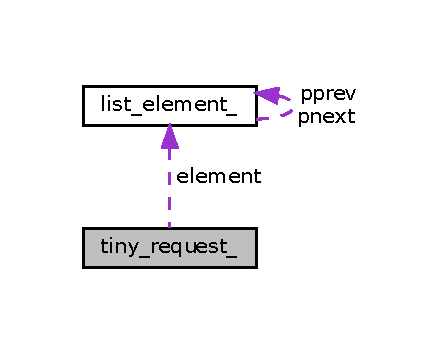
\includegraphics[width=212pt]{structtiny__request____coll__graph}
\end{center}
\end{figure}
\subsection*{Public Attributes}
\begin{DoxyCompactItemize}
\item 
\mbox{\Hypertarget{structtiny__request___a02c8fb6d26d0cfb0264423a1cb643159}\label{structtiny__request___a02c8fb6d26d0cfb0264423a1cb643159}} 
\hyperlink{structlist__element__}{list\+\_\+element} \hyperlink{structtiny__request___a02c8fb6d26d0cfb0264423a1cb643159}{element}
\begin{DoxyCompactList}\small\item\em This is base data for tiny lists. Must be first field in the structure. \end{DoxyCompactList}\item 
\mbox{\Hypertarget{structtiny__request___a019207b55569a48a82a2922dd3cc7eb2}\label{structtiny__request___a019207b55569a48a82a2922dd3cc7eb2}} 
uint8\+\_\+t \hyperlink{structtiny__request___a019207b55569a48a82a2922dd3cc7eb2}{state}
\begin{DoxyCompactList}\small\item\em state of the request \end{DoxyCompactList}\item 
\mbox{\Hypertarget{structtiny__request___aefa85d07e09d6772963532b6cf1ed125}\label{structtiny__request___aefa85d07e09d6772963532b6cf1ed125}} 
uint16\+\_\+t \hyperlink{structtiny__request___aefa85d07e09d6772963532b6cf1ed125}{uid}
\begin{DoxyCompactList}\small\item\em unique id of the sent packet \end{DoxyCompactList}\end{DoxyCompactItemize}


\subsection{Detailed Description}
defines type for tiny request list item 

The documentation for this struct was generated from the following file\+:\begin{DoxyCompactItemize}
\item 
src/proto/half\+\_\+duplex/tiny\+\_\+rq\+\_\+pool.\+h\end{DoxyCompactItemize}

\chapter{File Documentation}
\hypertarget{arduino_8dox}{}\section{src/arduino.dox File Reference}
\label{arduino_8dox}\index{src/arduino.\+dox@{src/arduino.\+dox}}


Arduino reated A\+PI.  




\subsection{Detailed Description}
Arduino reated A\+PI. 


\hypertarget{mainpage_8dox}{}\section{src/mainpage.dox File Reference}
\label{mainpage_8dox}\index{src/mainpage.\+dox@{src/mainpage.\+dox}}


Tiny Microcontroller Communication Protocol.  




\subsection{Detailed Description}
Tiny Microcontroller Communication Protocol. 


\hypertarget{tiny__fd_8h}{}\section{src/proto/fd/tiny\+\_\+fd.h File Reference}
\label{tiny__fd_8h}\index{src/proto/fd/tiny\+\_\+fd.\+h@{src/proto/fd/tiny\+\_\+fd.\+h}}


Tiny Protocol Full Duplex A\+PI.  


{\ttfamily \#include $<$stdint.\+h$>$}\newline
{\ttfamily \#include \char`\"{}proto/hdlc/tiny\+\_\+hdlc.\+h\char`\"{}}\newline
{\ttfamily \#include \char`\"{}proto/hal/tiny\+\_\+types.\+h\char`\"{}}\newline
Include dependency graph for tiny\+\_\+fd.\+h\+:
\nopagebreak
\begin{figure}[H]
\begin{center}
\leavevmode
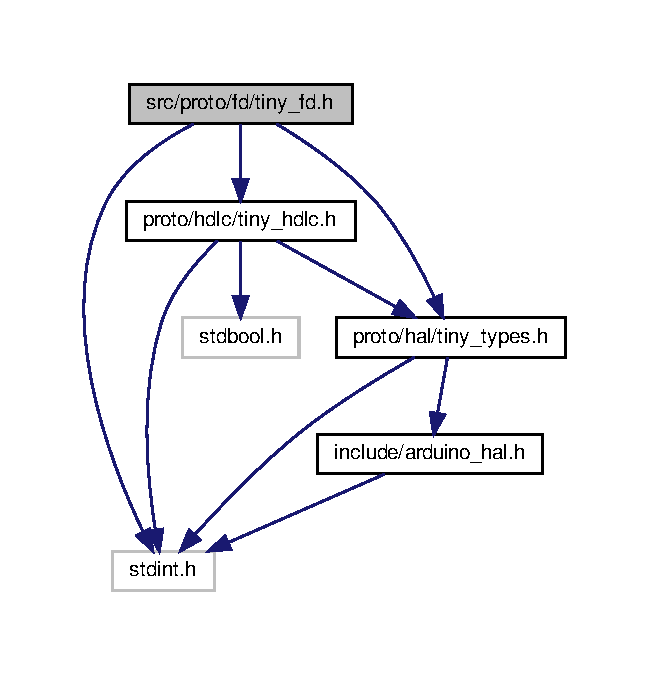
\includegraphics[width=333pt]{tiny__fd_8h__incl}
\end{center}
\end{figure}
This graph shows which files directly or indirectly include this file\+:
\nopagebreak
\begin{figure}[H]
\begin{center}
\leavevmode
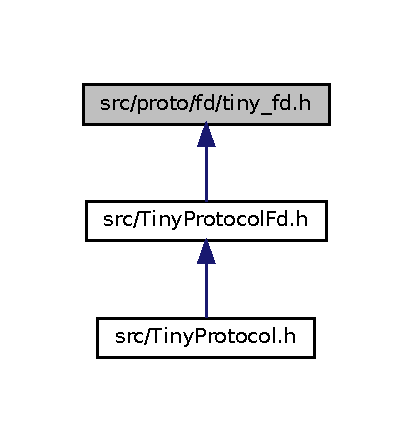
\includegraphics[width=198pt]{tiny__fd_8h__dep__incl}
\end{center}
\end{figure}
\subsection*{Classes}
\begin{DoxyCompactItemize}
\item 
struct \hyperlink{structSTinyFdInit__}{S\+Tiny\+Fd\+Init\+\_\+}
\end{DoxyCompactItemize}
\subsection*{Typedefs}
\begin{DoxyCompactItemize}
\item 
typedef struct tiny\+\_\+fd\+\_\+data\+\_\+t $\ast$ \hyperlink{tiny__fd_8h_a91e6b79431fe38570fb102701ef0b7e8}{tiny\+\_\+fd\+\_\+handle\+\_\+t}
\item 
typedef struct \hyperlink{structSTinyFdInit__}{S\+Tiny\+Fd\+Init\+\_\+} \hyperlink{tiny__fd_8h_ac931714d7bbe299856f4533fd1edb7f6}{S\+Tiny\+Fd\+Init}
\end{DoxyCompactItemize}
\subsection*{Functions}
\begin{DoxyCompactItemize}
\item 
int \hyperlink{group__FULL__DUPLEX__API_ga73c3e76cfbcd7b9bb8e1f7826175774b}{tiny\+\_\+fd\+\_\+init} (\hyperlink{tiny__fd_8h_a91e6b79431fe38570fb102701ef0b7e8}{tiny\+\_\+fd\+\_\+handle\+\_\+t} $\ast$handle, \hyperlink{tiny__fd_8h_ac931714d7bbe299856f4533fd1edb7f6}{S\+Tiny\+Fd\+Init} $\ast$init)
\begin{DoxyCompactList}\small\item\em Initialized communication for Tiny Full Duplex protocol. \end{DoxyCompactList}\item 
void \hyperlink{group__FULL__DUPLEX__API_ga11e470503e3359bc29a5bcb65a9771d5}{tiny\+\_\+fd\+\_\+close} (\hyperlink{tiny__fd_8h_a91e6b79431fe38570fb102701ef0b7e8}{tiny\+\_\+fd\+\_\+handle\+\_\+t} handle)
\begin{DoxyCompactList}\small\item\em stops Tiny Full Duplex state machine \end{DoxyCompactList}\item 
int \hyperlink{group__FULL__DUPLEX__API_ga601c9874a570331580856c1ea28f7914}{tiny\+\_\+fd\+\_\+run\+\_\+tx} (\hyperlink{tiny__fd_8h_a91e6b79431fe38570fb102701ef0b7e8}{tiny\+\_\+fd\+\_\+handle\+\_\+t} handle, uint16\+\_\+t timeout)
\begin{DoxyCompactList}\small\item\em runs tx processing for specified period of time. \end{DoxyCompactList}\item 
int \hyperlink{group__FULL__DUPLEX__API_gad31f944514aef01e27bc3ec67fdbe140}{tiny\+\_\+fd\+\_\+run\+\_\+rx} (\hyperlink{tiny__fd_8h_a91e6b79431fe38570fb102701ef0b7e8}{tiny\+\_\+fd\+\_\+handle\+\_\+t} handle, uint16\+\_\+t timeout)
\begin{DoxyCompactList}\small\item\em runs rx processing for specified period of time. \end{DoxyCompactList}\item 
int \hyperlink{group__FULL__DUPLEX__API_ga490157ee98ea6148f99a5bb1f26c5f60}{tiny\+\_\+fd\+\_\+send} (\hyperlink{tiny__fd_8h_a91e6b79431fe38570fb102701ef0b7e8}{tiny\+\_\+fd\+\_\+handle\+\_\+t} handle, const void $\ast$buf, int len)
\begin{DoxyCompactList}\small\item\em Sends userdata over full-\/duplex protocol. \end{DoxyCompactList}\item 
int \hyperlink{group__FULL__DUPLEX__API_ga19789bea5b5acd68804773f0d6b0e3f7}{tiny\+\_\+fd\+\_\+buffer\+\_\+size\+\_\+by\+\_\+mtu} (int mtu, int max\+\_\+tx\+\_\+frames)
\end{DoxyCompactItemize}


\subsection{Detailed Description}
Tiny Protocol Full Duplex A\+PI. 

This is Tiny Half-\/\+Duplex protocol implementation for microcontrollers. It is built on top of Tiny Protocol (tiny\+\_\+layer2.\+c)

Implements full duplex asynchronous ballanced mode (A\+BM) 

\subsection{Typedef Documentation}
\mbox{\Hypertarget{tiny__fd_8h_ac931714d7bbe299856f4533fd1edb7f6}\label{tiny__fd_8h_ac931714d7bbe299856f4533fd1edb7f6}} 
\index{tiny\+\_\+fd.\+h@{tiny\+\_\+fd.\+h}!S\+Tiny\+Fd\+Init@{S\+Tiny\+Fd\+Init}}
\index{S\+Tiny\+Fd\+Init@{S\+Tiny\+Fd\+Init}!tiny\+\_\+fd.\+h@{tiny\+\_\+fd.\+h}}
\subsubsection{\texorpdfstring{S\+Tiny\+Fd\+Init}{STinyFdInit}}
{\footnotesize\ttfamily typedef struct \hyperlink{structSTinyFdInit__}{S\+Tiny\+Fd\+Init\+\_\+}  \hyperlink{tiny__fd_8h_ac931714d7bbe299856f4533fd1edb7f6}{S\+Tiny\+Fd\+Init}}

This structure is used for initialization of Tiny Full Duplex protocol. \mbox{\Hypertarget{tiny__fd_8h_a91e6b79431fe38570fb102701ef0b7e8}\label{tiny__fd_8h_a91e6b79431fe38570fb102701ef0b7e8}} 
\index{tiny\+\_\+fd.\+h@{tiny\+\_\+fd.\+h}!tiny\+\_\+fd\+\_\+handle\+\_\+t@{tiny\+\_\+fd\+\_\+handle\+\_\+t}}
\index{tiny\+\_\+fd\+\_\+handle\+\_\+t@{tiny\+\_\+fd\+\_\+handle\+\_\+t}!tiny\+\_\+fd.\+h@{tiny\+\_\+fd.\+h}}
\subsubsection{\texorpdfstring{tiny\+\_\+fd\+\_\+handle\+\_\+t}{tiny\_fd\_handle\_t}}
{\footnotesize\ttfamily typedef struct tiny\+\_\+fd\+\_\+data\+\_\+t$\ast$ \hyperlink{tiny__fd_8h_a91e6b79431fe38570fb102701ef0b7e8}{tiny\+\_\+fd\+\_\+handle\+\_\+t}}

This handle points to service data, required for full-\/duplex functioning. 
\hypertarget{tiny__types_8h}{}\section{src/proto/hal/tiny\+\_\+types.h File Reference}
\label{tiny__types_8h}\index{src/proto/hal/tiny\+\_\+types.\+h@{src/proto/hal/tiny\+\_\+types.\+h}}


Tiny protocol Types.  


{\ttfamily \#include \char`\"{}include/arduino\+\_\+hal.\+h\char`\"{}}\newline
{\ttfamily \#include $<$stdint.\+h$>$}\newline
Include dependency graph for tiny\+\_\+types.\+h\+:
\nopagebreak
\begin{figure}[H]
\begin{center}
\leavevmode
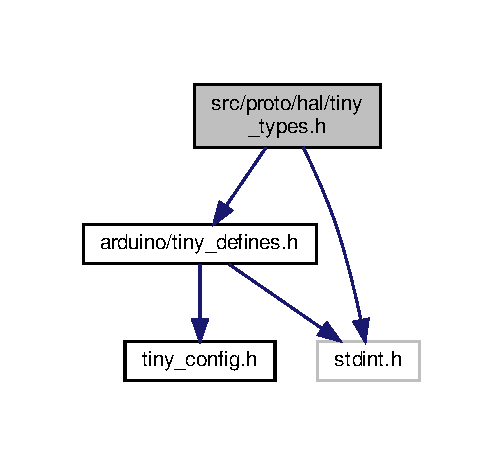
\includegraphics[width=220pt]{tiny__types_8h__incl}
\end{center}
\end{figure}
This graph shows which files directly or indirectly include this file\+:
\nopagebreak
\begin{figure}[H]
\begin{center}
\leavevmode
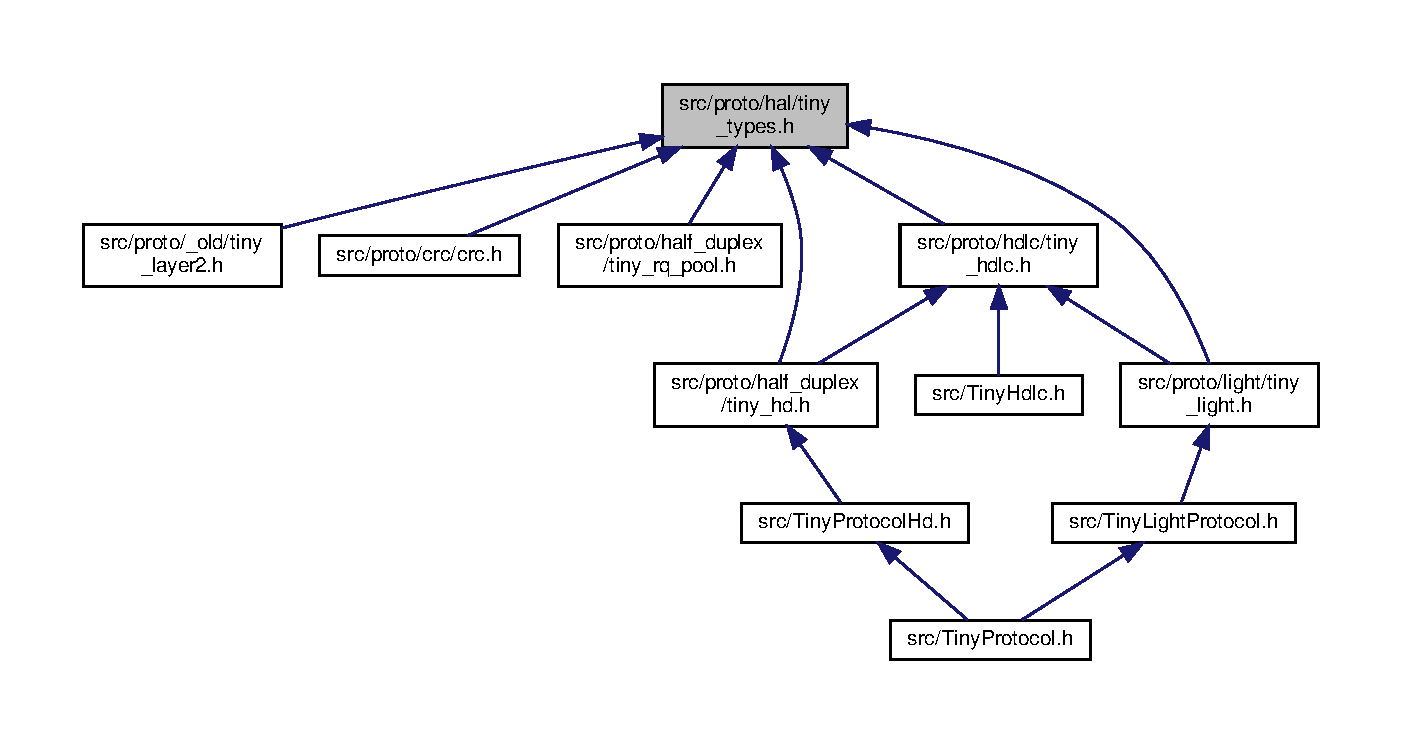
\includegraphics[width=350pt]{tiny__types_8h__dep__incl}
\end{center}
\end{figure}
\subsection*{Classes}
\begin{DoxyCompactItemize}
\item 
struct \hyperlink{structSTinyStats}{S\+Tiny\+Stats}
\end{DoxyCompactItemize}
\subsection*{Macros}
\begin{DoxyCompactItemize}
\item 
\#define \hyperlink{group__ERROR__FLAGS_ga16cd043c890ed1fa381b3a20f75a626c}{T\+I\+N\+Y\+\_\+\+S\+U\+C\+C\+E\+SS}~(0)
\begin{DoxyCompactList}\small\item\em Tiny operation successful. Only tiny\+\_\+send\+\_\+start and tiny\+\_\+read\+\_\+start functions return this code. \end{DoxyCompactList}\item 
\#define \hyperlink{group__ERROR__FLAGS_ga84e6ca143550038e1a71cf36078d1926}{T\+I\+N\+Y\+\_\+\+E\+R\+R\+\_\+\+F\+A\+I\+L\+ED}~(-\/1)
\begin{DoxyCompactList}\small\item\em Timeout. \end{DoxyCompactList}\item 
\#define \hyperlink{group__ERROR__FLAGS_gac9ba8076a1eb8613e8d1f07629ff0cd1}{T\+I\+N\+Y\+\_\+\+E\+R\+R\+\_\+\+T\+I\+M\+E\+O\+UT}~(-\/2)
\begin{DoxyCompactList}\small\item\em Timeout happened. The function must be called once again. \end{DoxyCompactList}\item 
\#define \hyperlink{group__ERROR__FLAGS_ga7bbe7440d11ad304b0af68e011f4eab7}{T\+I\+N\+Y\+\_\+\+E\+R\+R\+\_\+\+D\+A\+T\+A\+\_\+\+T\+O\+O\+\_\+\+L\+A\+R\+GE}~(-\/3)
\begin{DoxyCompactList}\small\item\em Data too large to fit the user buffer. \end{DoxyCompactList}\item 
\#define \hyperlink{group__ERROR__FLAGS_ga541a9e67a84e39595ad647d641c4df2e}{T\+I\+N\+Y\+\_\+\+E\+R\+R\+\_\+\+I\+N\+V\+A\+L\+I\+D\+\_\+\+D\+A\+TA}~(-\/4)
\begin{DoxyCompactList}\small\item\em Some invalid data passed to Tiny A\+PI function. \end{DoxyCompactList}\item 
\#define \hyperlink{group__ERROR__FLAGS_ga9b3e170e1c6ce269f216ef4a1ac61995}{T\+I\+N\+Y\+\_\+\+E\+R\+R\+\_\+\+B\+U\+SY}~(-\/5)
\begin{DoxyCompactList}\small\item\em A\+PI function detected that operation cannot be performed right now. \end{DoxyCompactList}\item 
\#define \hyperlink{group__ERROR__FLAGS_gae1949de45d9c478830dad9c9b996193a}{T\+I\+N\+Y\+\_\+\+E\+R\+R\+\_\+\+O\+U\+T\+\_\+\+O\+F\+\_\+\+S\+Y\+NC}~(-\/6)
\begin{DoxyCompactList}\small\item\em Out of sync -\/ received some data, which are not part of the frame (tiny\+\_\+read) \end{DoxyCompactList}\item 
\#define \hyperlink{group__ERROR__FLAGS_gab15347e8e9f90d709d94d9c151d505b7}{T\+I\+N\+Y\+\_\+\+E\+R\+R\+\_\+\+A\+G\+A\+IN}~(-\/7)
\begin{DoxyCompactList}\small\item\em No data for now, need to retry reading once again. \end{DoxyCompactList}\item 
\#define \hyperlink{group__ERROR__FLAGS_ga618f7dd6cead76223e60300212712871}{T\+I\+N\+Y\+\_\+\+E\+R\+R\+\_\+\+W\+R\+O\+N\+G\+\_\+\+C\+RC}~(-\/8)
\begin{DoxyCompactList}\small\item\em Invalid crc field of incoming frame. \end{DoxyCompactList}\item 
\#define \hyperlink{group__FLAGS__GROUP_gadadd60eb21d7949e6d097ad36aab9b2e}{T\+I\+N\+Y\+\_\+\+F\+L\+A\+G\+\_\+\+N\+O\+\_\+\+W\+A\+IT}~(0)
\begin{DoxyCompactList}\small\item\em This flag makes tiny A\+PI functions perform as non-\/blocking. \end{DoxyCompactList}\item 
\#define \hyperlink{group__FLAGS__GROUP_gae41123cfeed375e618a4152c9bbd0d6d}{T\+I\+N\+Y\+\_\+\+F\+L\+A\+G\+\_\+\+R\+E\+A\+D\+\_\+\+A\+LL}~(1)
\begin{DoxyCompactList}\small\item\em This flag makes tiny\+\_\+read function to read whole frame event if it doesn\textquotesingle{}t fit the buffer. \end{DoxyCompactList}\item 
\#define \hyperlink{group__FLAGS__GROUP_ga593e3353339a36dcd0746057e2864958}{T\+I\+N\+Y\+\_\+\+F\+L\+A\+G\+\_\+\+L\+O\+C\+K\+\_\+\+S\+E\+ND}~(2)
\begin{DoxyCompactList}\small\item\em Informs advanced A\+PI that caller wants to start transmit new frame to the channel. \end{DoxyCompactList}\item 
\#define \hyperlink{group__FLAGS__GROUP_ga3a34267804581c5709d03f52d232b307}{T\+I\+N\+Y\+\_\+\+F\+L\+A\+G\+\_\+\+W\+A\+I\+T\+\_\+\+F\+O\+R\+E\+V\+ER}~(0x80)
\begin{DoxyCompactList}\small\item\em This flag makes tiny A\+PI functions perform in blocking mode. \end{DoxyCompactList}\item 
\mbox{\Hypertarget{tiny__types_8h_a27b8fac677976106d127489aed30c6ea}\label{tiny__types_8h_a27b8fac677976106d127489aed30c6ea}} 
\#define \hyperlink{tiny__types_8h_a27b8fac677976106d127489aed30c6ea}{E\+V\+E\+N\+T\+\_\+\+B\+I\+S\+\_\+\+A\+LL}~0x\+FF
\begin{DoxyCompactList}\small\item\em All bits supported by tiny protocol H\+AL events. \end{DoxyCompactList}\item 
\mbox{\Hypertarget{tiny__types_8h_ad1077ed0be1ef067bb34790e17829eff}\label{tiny__types_8h_ad1077ed0be1ef067bb34790e17829eff}} 
\#define \hyperlink{tiny__types_8h_ad1077ed0be1ef067bb34790e17829eff}{E\+V\+E\+N\+T\+\_\+\+B\+I\+T\+S\+\_\+\+C\+L\+E\+AR}~1
\begin{DoxyCompactList}\small\item\em Flag, used in \hyperlink{tiny__types_8h_aa9f8404c92b31f6df4b2b929ad54588b}{tiny\+\_\+events\+\_\+wait()} \end{DoxyCompactList}\item 
\mbox{\Hypertarget{tiny__types_8h_aa5326a270b651a7a0d23e219e63de174}\label{tiny__types_8h_aa5326a270b651a7a0d23e219e63de174}} 
\#define \hyperlink{tiny__types_8h_aa5326a270b651a7a0d23e219e63de174}{E\+V\+E\+N\+T\+\_\+\+B\+I\+T\+S\+\_\+\+L\+E\+A\+VE}~0
\begin{DoxyCompactList}\small\item\em Flag, used in \hyperlink{tiny__types_8h_aa9f8404c92b31f6df4b2b929ad54588b}{tiny\+\_\+events\+\_\+wait()} \end{DoxyCompactList}\end{DoxyCompactItemize}
\subsection*{Typedefs}
\begin{DoxyCompactItemize}
\item 
typedef int($\ast$ \hyperlink{tiny__types_8h_aafd634660bba76cace57a8f9b01e044d}{write\+\_\+block\+\_\+cb\+\_\+t}) (void $\ast$pdata, const void $\ast$buffer, int size)
\item 
typedef int($\ast$ \hyperlink{tiny__types_8h_a15bec127d9ee63658563d62e92b5261b}{read\+\_\+block\+\_\+cb\+\_\+t}) (void $\ast$pdata, void $\ast$buffer, int size)
\item 
typedef void($\ast$ \hyperlink{tiny__types_8h_ad6bf709565b8aecb9e6ecf196f219d54}{on\+\_\+frame\+\_\+cb\+\_\+t}) (void $\ast$handle, uint16\+\_\+t uid, uint8\+\_\+t $\ast$pdata, int size)
\end{DoxyCompactItemize}
\subsection*{Functions}
\begin{DoxyCompactItemize}
\item 
void \hyperlink{tiny__types_8h_ad33eeb8054f4677e4441d3602d33b734}{tiny\+\_\+mutex\+\_\+create} (tiny\+\_\+mutex\+\_\+t $\ast$mutex)
\item 
void \hyperlink{tiny__types_8h_ae469a75fca0339d7455583955920647c}{tiny\+\_\+mutex\+\_\+destroy} (tiny\+\_\+mutex\+\_\+t $\ast$mutex)
\item 
void \hyperlink{tiny__types_8h_a62207a0f8490d55b9fc529a8773bcf0a}{tiny\+\_\+mutex\+\_\+lock} (tiny\+\_\+mutex\+\_\+t $\ast$mutex)
\item 
uint8\+\_\+t \hyperlink{tiny__types_8h_a3c5ef9a47c4bcb2d4f7f59ec91b8dc68}{tiny\+\_\+mutex\+\_\+try\+\_\+lock} (tiny\+\_\+mutex\+\_\+t $\ast$mutex)
\item 
void \hyperlink{tiny__types_8h_aef1ccb057b482b334079565a0e75eb6c}{tiny\+\_\+mutex\+\_\+unlock} (tiny\+\_\+mutex\+\_\+t $\ast$mutex)
\item 
void \hyperlink{tiny__types_8h_a8f8dca30c01b01d94c80babecd4396a7}{tiny\+\_\+events\+\_\+create} (tiny\+\_\+events\+\_\+t $\ast$events)
\item 
void \hyperlink{tiny__types_8h_a786fc845ce2ff24d7633d41e2524785c}{tiny\+\_\+events\+\_\+destroy} (tiny\+\_\+events\+\_\+t $\ast$events)
\item 
uint8\+\_\+t \hyperlink{tiny__types_8h_aa9f8404c92b31f6df4b2b929ad54588b}{tiny\+\_\+events\+\_\+wait} (tiny\+\_\+events\+\_\+t $\ast$event, uint8\+\_\+t bits, uint8\+\_\+t clear, uint32\+\_\+t timeout)
\item 
void \hyperlink{tiny__types_8h_a7d57419d88bfa7496e9d743c7831590a}{tiny\+\_\+events\+\_\+set} (tiny\+\_\+events\+\_\+t $\ast$event, uint8\+\_\+t bits)
\item 
void \hyperlink{tiny__types_8h_a478739391a83f06f56a5beaef649410c}{tiny\+\_\+events\+\_\+clear} (tiny\+\_\+events\+\_\+t $\ast$event, uint8\+\_\+t bits)
\item 
void \hyperlink{tiny__types_8h_ae024e04660c8b9a9a231965f7aee5112}{tiny\+\_\+sleep} (uint32\+\_\+t ms)
\item 
uint32\+\_\+t \hyperlink{tiny__types_8h_a43bebe1b00a80373afd7b8061bf742fe}{tiny\+\_\+millis} ()
\item 
void \hyperlink{tiny__types_8h_a3c7a23a4fe40e7c33691618b7ad91e87}{tiny\+\_\+log\+\_\+level} (uint8\+\_\+t level)
\end{DoxyCompactItemize}


\subsection{Detailed Description}
Tiny protocol Types. 

This is Tiny protocol implementation for microcontrollers 

\subsection{Typedef Documentation}
\mbox{\Hypertarget{tiny__types_8h_ad6bf709565b8aecb9e6ecf196f219d54}\label{tiny__types_8h_ad6bf709565b8aecb9e6ecf196f219d54}} 
\index{tiny\+\_\+types.\+h@{tiny\+\_\+types.\+h}!on\+\_\+frame\+\_\+cb\+\_\+t@{on\+\_\+frame\+\_\+cb\+\_\+t}}
\index{on\+\_\+frame\+\_\+cb\+\_\+t@{on\+\_\+frame\+\_\+cb\+\_\+t}!tiny\+\_\+types.\+h@{tiny\+\_\+types.\+h}}
\subsubsection{\texorpdfstring{on\+\_\+frame\+\_\+cb\+\_\+t}{on\_frame\_cb\_t}}
{\footnotesize\ttfamily typedef void($\ast$ on\+\_\+frame\+\_\+cb\+\_\+t) (void $\ast$handle, uint16\+\_\+t uid, uint8\+\_\+t $\ast$pdata, int size)}

on\+\_\+frame\+\_\+cb\+\_\+t is a callback function, which is called every time new frame is received, or sent. refer to tiny\+\_\+set\+\_\+callbacks 
\begin{DoxyParams}{Parameters}
{\em handle} & -\/ handle of Tiny. \\
\hline
{\em uid} & -\/ U\+ID of the received frame or sent frame (if uids are enabled). \\
\hline
{\em pdata} & -\/ data received over Tiny Protocol. \\
\hline
{\em size} & -\/ size of data received. \\
\hline
\end{DoxyParams}
\begin{DoxyReturn}{Returns}
None. 
\end{DoxyReturn}
\begin{DoxySeeAlso}{See also}
tiny\+\_\+set\+\_\+callbacks 
\end{DoxySeeAlso}
\mbox{\Hypertarget{tiny__types_8h_a15bec127d9ee63658563d62e92b5261b}\label{tiny__types_8h_a15bec127d9ee63658563d62e92b5261b}} 
\index{tiny\+\_\+types.\+h@{tiny\+\_\+types.\+h}!read\+\_\+block\+\_\+cb\+\_\+t@{read\+\_\+block\+\_\+cb\+\_\+t}}
\index{read\+\_\+block\+\_\+cb\+\_\+t@{read\+\_\+block\+\_\+cb\+\_\+t}!tiny\+\_\+types.\+h@{tiny\+\_\+types.\+h}}
\subsubsection{\texorpdfstring{read\+\_\+block\+\_\+cb\+\_\+t}{read\_block\_cb\_t}}
{\footnotesize\ttfamily typedef int($\ast$ read\+\_\+block\+\_\+cb\+\_\+t) (void $\ast$pdata, void $\ast$buffer, int size)}

The function reads data from communication channel. 
\begin{DoxyParams}{Parameters}
{\em pdata} & -\/ pointer to user private data. -\/ absent in Arduino version \\
\hline
{\em buffer} & -\/ pointer to a buffer to read data to from the channel. \\
\hline
{\em size} & -\/ maximum size of the buffer. \\
\hline
\end{DoxyParams}
\begin{DoxySeeAlso}{See also}
\hyperlink{tiny__types_8h_aafd634660bba76cace57a8f9b01e044d}{write\+\_\+block\+\_\+cb\+\_\+t} 
\end{DoxySeeAlso}
\begin{DoxyReturn}{Returns}
the function must return negative value in case of error or number of bytes actually read or zero. 
\end{DoxyReturn}
\mbox{\Hypertarget{tiny__types_8h_aafd634660bba76cace57a8f9b01e044d}\label{tiny__types_8h_aafd634660bba76cace57a8f9b01e044d}} 
\index{tiny\+\_\+types.\+h@{tiny\+\_\+types.\+h}!write\+\_\+block\+\_\+cb\+\_\+t@{write\+\_\+block\+\_\+cb\+\_\+t}}
\index{write\+\_\+block\+\_\+cb\+\_\+t@{write\+\_\+block\+\_\+cb\+\_\+t}!tiny\+\_\+types.\+h@{tiny\+\_\+types.\+h}}
\subsubsection{\texorpdfstring{write\+\_\+block\+\_\+cb\+\_\+t}{write\_block\_cb\_t}}
{\footnotesize\ttfamily typedef int($\ast$ write\+\_\+block\+\_\+cb\+\_\+t) (void $\ast$pdata, const void $\ast$buffer, int size)}

The function writes data to communication channel port. 
\begin{DoxyParams}{Parameters}
{\em pdata} & -\/ pointer to user private data -\/ absent in Arduino version \\
\hline
{\em buffer} & -\/ pointer to the data to send to channel. \\
\hline
{\em size} & -\/ size of data to write. \\
\hline
\end{DoxyParams}
\begin{DoxySeeAlso}{See also}
\hyperlink{tiny__types_8h_a15bec127d9ee63658563d62e92b5261b}{read\+\_\+block\+\_\+cb\+\_\+t} 
\end{DoxySeeAlso}
\begin{DoxyReturn}{Returns}
the function must return negative value in case of error or number of bytes written or zero. 
\end{DoxyReturn}


\subsection{Function Documentation}
\mbox{\Hypertarget{tiny__types_8h_a478739391a83f06f56a5beaef649410c}\label{tiny__types_8h_a478739391a83f06f56a5beaef649410c}} 
\index{tiny\+\_\+types.\+h@{tiny\+\_\+types.\+h}!tiny\+\_\+events\+\_\+clear@{tiny\+\_\+events\+\_\+clear}}
\index{tiny\+\_\+events\+\_\+clear@{tiny\+\_\+events\+\_\+clear}!tiny\+\_\+types.\+h@{tiny\+\_\+types.\+h}}
\subsubsection{\texorpdfstring{tiny\+\_\+events\+\_\+clear()}{tiny\_events\_clear()}}
{\footnotesize\ttfamily void tiny\+\_\+events\+\_\+clear (\begin{DoxyParamCaption}\item[{tiny\+\_\+events\+\_\+t $\ast$}]{event,  }\item[{uint8\+\_\+t}]{bits }\end{DoxyParamCaption})}

Clears bits for cross-\/platform event group object. 
\begin{DoxyParams}{Parameters}
{\em event} & pointer to tiny\+\_\+event\+\_\+t variable. \\
\hline
{\em bits} & bits to clear \\
\hline
\end{DoxyParams}
\mbox{\Hypertarget{tiny__types_8h_a8f8dca30c01b01d94c80babecd4396a7}\label{tiny__types_8h_a8f8dca30c01b01d94c80babecd4396a7}} 
\index{tiny\+\_\+types.\+h@{tiny\+\_\+types.\+h}!tiny\+\_\+events\+\_\+create@{tiny\+\_\+events\+\_\+create}}
\index{tiny\+\_\+events\+\_\+create@{tiny\+\_\+events\+\_\+create}!tiny\+\_\+types.\+h@{tiny\+\_\+types.\+h}}
\subsubsection{\texorpdfstring{tiny\+\_\+events\+\_\+create()}{tiny\_events\_create()}}
{\footnotesize\ttfamily void tiny\+\_\+events\+\_\+create (\begin{DoxyParamCaption}\item[{tiny\+\_\+events\+\_\+t $\ast$}]{events }\end{DoxyParamCaption})}

Creates cross platform event group object. 
\begin{DoxyParams}{Parameters}
{\em events} & pointer to tiny\+\_\+event\+\_\+t variable. \\
\hline
\end{DoxyParams}
\mbox{\Hypertarget{tiny__types_8h_a786fc845ce2ff24d7633d41e2524785c}\label{tiny__types_8h_a786fc845ce2ff24d7633d41e2524785c}} 
\index{tiny\+\_\+types.\+h@{tiny\+\_\+types.\+h}!tiny\+\_\+events\+\_\+destroy@{tiny\+\_\+events\+\_\+destroy}}
\index{tiny\+\_\+events\+\_\+destroy@{tiny\+\_\+events\+\_\+destroy}!tiny\+\_\+types.\+h@{tiny\+\_\+types.\+h}}
\subsubsection{\texorpdfstring{tiny\+\_\+events\+\_\+destroy()}{tiny\_events\_destroy()}}
{\footnotesize\ttfamily void tiny\+\_\+events\+\_\+destroy (\begin{DoxyParamCaption}\item[{tiny\+\_\+events\+\_\+t $\ast$}]{events }\end{DoxyParamCaption})}

Destroys cross platform event group object. 
\begin{DoxyParams}{Parameters}
{\em events} & pointer to tiny\+\_\+event\+\_\+t variable. \\
\hline
\end{DoxyParams}
\mbox{\Hypertarget{tiny__types_8h_a7d57419d88bfa7496e9d743c7831590a}\label{tiny__types_8h_a7d57419d88bfa7496e9d743c7831590a}} 
\index{tiny\+\_\+types.\+h@{tiny\+\_\+types.\+h}!tiny\+\_\+events\+\_\+set@{tiny\+\_\+events\+\_\+set}}
\index{tiny\+\_\+events\+\_\+set@{tiny\+\_\+events\+\_\+set}!tiny\+\_\+types.\+h@{tiny\+\_\+types.\+h}}
\subsubsection{\texorpdfstring{tiny\+\_\+events\+\_\+set()}{tiny\_events\_set()}}
{\footnotesize\ttfamily void tiny\+\_\+events\+\_\+set (\begin{DoxyParamCaption}\item[{tiny\+\_\+events\+\_\+t $\ast$}]{event,  }\item[{uint8\+\_\+t}]{bits }\end{DoxyParamCaption})}

Sets bits for cross-\/platform event group object. 
\begin{DoxyParams}{Parameters}
{\em event} & pointer to tiny\+\_\+event\+\_\+t variable. \\
\hline
{\em bits} & bits to set \\
\hline
\end{DoxyParams}
\mbox{\Hypertarget{tiny__types_8h_aa9f8404c92b31f6df4b2b929ad54588b}\label{tiny__types_8h_aa9f8404c92b31f6df4b2b929ad54588b}} 
\index{tiny\+\_\+types.\+h@{tiny\+\_\+types.\+h}!tiny\+\_\+events\+\_\+wait@{tiny\+\_\+events\+\_\+wait}}
\index{tiny\+\_\+events\+\_\+wait@{tiny\+\_\+events\+\_\+wait}!tiny\+\_\+types.\+h@{tiny\+\_\+types.\+h}}
\subsubsection{\texorpdfstring{tiny\+\_\+events\+\_\+wait()}{tiny\_events\_wait()}}
{\footnotesize\ttfamily uint8\+\_\+t tiny\+\_\+events\+\_\+wait (\begin{DoxyParamCaption}\item[{tiny\+\_\+events\+\_\+t $\ast$}]{event,  }\item[{uint8\+\_\+t}]{bits,  }\item[{uint8\+\_\+t}]{clear,  }\item[{uint32\+\_\+t}]{timeout }\end{DoxyParamCaption})}

Waits until any of specified bits is set or timeout. 
\begin{DoxyParams}{Parameters}
{\em event} & pointer to tiny\+\_\+event\+\_\+t variable. \\
\hline
{\em bits} & bits to wait for \\
\hline
{\em clear} & flags E\+V\+E\+N\+T\+\_\+\+B\+I\+T\+S\+\_\+\+C\+L\+E\+AR or E\+V\+E\+N\+T\+\_\+\+B\+I\+T\+S\+\_\+\+L\+E\+A\+VE \\
\hline
{\em timeout} & timeout in milliseconds to wait \\
\hline
\end{DoxyParams}
\begin{DoxyReturn}{Returns}
0 on timeout list of bits from the input argument, which were set 
\end{DoxyReturn}
\mbox{\Hypertarget{tiny__types_8h_a3c7a23a4fe40e7c33691618b7ad91e87}\label{tiny__types_8h_a3c7a23a4fe40e7c33691618b7ad91e87}} 
\index{tiny\+\_\+types.\+h@{tiny\+\_\+types.\+h}!tiny\+\_\+log\+\_\+level@{tiny\+\_\+log\+\_\+level}}
\index{tiny\+\_\+log\+\_\+level@{tiny\+\_\+log\+\_\+level}!tiny\+\_\+types.\+h@{tiny\+\_\+types.\+h}}
\subsubsection{\texorpdfstring{tiny\+\_\+log\+\_\+level()}{tiny\_log\_level()}}
{\footnotesize\ttfamily void tiny\+\_\+log\+\_\+level (\begin{DoxyParamCaption}\item[{uint8\+\_\+t}]{level }\end{DoxyParamCaption})}

Sets logging level if tiny library is compiled with logs 
\begin{DoxyParams}{Parameters}
{\em level} & log level to set, or 0 to disable logs \\
\hline
\end{DoxyParams}
\mbox{\Hypertarget{tiny__types_8h_a43bebe1b00a80373afd7b8061bf742fe}\label{tiny__types_8h_a43bebe1b00a80373afd7b8061bf742fe}} 
\index{tiny\+\_\+types.\+h@{tiny\+\_\+types.\+h}!tiny\+\_\+millis@{tiny\+\_\+millis}}
\index{tiny\+\_\+millis@{tiny\+\_\+millis}!tiny\+\_\+types.\+h@{tiny\+\_\+types.\+h}}
\subsubsection{\texorpdfstring{tiny\+\_\+millis()}{tiny\_millis()}}
{\footnotesize\ttfamily uint32\+\_\+t tiny\+\_\+millis (\begin{DoxyParamCaption}{ }\end{DoxyParamCaption})}

Returns timestamp in milliseconds since system started up. \mbox{\Hypertarget{tiny__types_8h_ad33eeb8054f4677e4441d3602d33b734}\label{tiny__types_8h_ad33eeb8054f4677e4441d3602d33b734}} 
\index{tiny\+\_\+types.\+h@{tiny\+\_\+types.\+h}!tiny\+\_\+mutex\+\_\+create@{tiny\+\_\+mutex\+\_\+create}}
\index{tiny\+\_\+mutex\+\_\+create@{tiny\+\_\+mutex\+\_\+create}!tiny\+\_\+types.\+h@{tiny\+\_\+types.\+h}}
\subsubsection{\texorpdfstring{tiny\+\_\+mutex\+\_\+create()}{tiny\_mutex\_create()}}
{\footnotesize\ttfamily void tiny\+\_\+mutex\+\_\+create (\begin{DoxyParamCaption}\item[{tiny\+\_\+mutex\+\_\+t $\ast$}]{mutex }\end{DoxyParamCaption})}

Creates cross-\/platform mutex. 
\begin{DoxyParams}{Parameters}
{\em mutex} & pointer to tiny\+\_\+mutex\+\_\+t variable. \\
\hline
\end{DoxyParams}
\mbox{\Hypertarget{tiny__types_8h_ae469a75fca0339d7455583955920647c}\label{tiny__types_8h_ae469a75fca0339d7455583955920647c}} 
\index{tiny\+\_\+types.\+h@{tiny\+\_\+types.\+h}!tiny\+\_\+mutex\+\_\+destroy@{tiny\+\_\+mutex\+\_\+destroy}}
\index{tiny\+\_\+mutex\+\_\+destroy@{tiny\+\_\+mutex\+\_\+destroy}!tiny\+\_\+types.\+h@{tiny\+\_\+types.\+h}}
\subsubsection{\texorpdfstring{tiny\+\_\+mutex\+\_\+destroy()}{tiny\_mutex\_destroy()}}
{\footnotesize\ttfamily void tiny\+\_\+mutex\+\_\+destroy (\begin{DoxyParamCaption}\item[{tiny\+\_\+mutex\+\_\+t $\ast$}]{mutex }\end{DoxyParamCaption})}

Destroys cross-\/platform mutex. 
\begin{DoxyParams}{Parameters}
{\em mutex} & pointer to tiny\+\_\+mutex\+\_\+t variable. \\
\hline
\end{DoxyParams}
\mbox{\Hypertarget{tiny__types_8h_a62207a0f8490d55b9fc529a8773bcf0a}\label{tiny__types_8h_a62207a0f8490d55b9fc529a8773bcf0a}} 
\index{tiny\+\_\+types.\+h@{tiny\+\_\+types.\+h}!tiny\+\_\+mutex\+\_\+lock@{tiny\+\_\+mutex\+\_\+lock}}
\index{tiny\+\_\+mutex\+\_\+lock@{tiny\+\_\+mutex\+\_\+lock}!tiny\+\_\+types.\+h@{tiny\+\_\+types.\+h}}
\subsubsection{\texorpdfstring{tiny\+\_\+mutex\+\_\+lock()}{tiny\_mutex\_lock()}}
{\footnotesize\ttfamily void tiny\+\_\+mutex\+\_\+lock (\begin{DoxyParamCaption}\item[{tiny\+\_\+mutex\+\_\+t $\ast$}]{mutex }\end{DoxyParamCaption})}

Locks cross-\/platform mutex. 
\begin{DoxyParams}{Parameters}
{\em mutex} & pointer to tiny\+\_\+mutex\+\_\+t variable. \\
\hline
\end{DoxyParams}
\mbox{\Hypertarget{tiny__types_8h_a3c5ef9a47c4bcb2d4f7f59ec91b8dc68}\label{tiny__types_8h_a3c5ef9a47c4bcb2d4f7f59ec91b8dc68}} 
\index{tiny\+\_\+types.\+h@{tiny\+\_\+types.\+h}!tiny\+\_\+mutex\+\_\+try\+\_\+lock@{tiny\+\_\+mutex\+\_\+try\+\_\+lock}}
\index{tiny\+\_\+mutex\+\_\+try\+\_\+lock@{tiny\+\_\+mutex\+\_\+try\+\_\+lock}!tiny\+\_\+types.\+h@{tiny\+\_\+types.\+h}}
\subsubsection{\texorpdfstring{tiny\+\_\+mutex\+\_\+try\+\_\+lock()}{tiny\_mutex\_try\_lock()}}
{\footnotesize\ttfamily uint8\+\_\+t tiny\+\_\+mutex\+\_\+try\+\_\+lock (\begin{DoxyParamCaption}\item[{tiny\+\_\+mutex\+\_\+t $\ast$}]{mutex }\end{DoxyParamCaption})}

Attempts to lock cross-\/platform mutex. 
\begin{DoxyParams}{Parameters}
{\em mutex} & pointer to tiny\+\_\+mutex\+\_\+t variable. \\
\hline
\end{DoxyParams}
\begin{DoxyReturn}{Returns}
0 if failed to lock 1 if success 
\end{DoxyReturn}
\mbox{\Hypertarget{tiny__types_8h_aef1ccb057b482b334079565a0e75eb6c}\label{tiny__types_8h_aef1ccb057b482b334079565a0e75eb6c}} 
\index{tiny\+\_\+types.\+h@{tiny\+\_\+types.\+h}!tiny\+\_\+mutex\+\_\+unlock@{tiny\+\_\+mutex\+\_\+unlock}}
\index{tiny\+\_\+mutex\+\_\+unlock@{tiny\+\_\+mutex\+\_\+unlock}!tiny\+\_\+types.\+h@{tiny\+\_\+types.\+h}}
\subsubsection{\texorpdfstring{tiny\+\_\+mutex\+\_\+unlock()}{tiny\_mutex\_unlock()}}
{\footnotesize\ttfamily void tiny\+\_\+mutex\+\_\+unlock (\begin{DoxyParamCaption}\item[{tiny\+\_\+mutex\+\_\+t $\ast$}]{mutex }\end{DoxyParamCaption})}

Unlocks cross-\/platform mutex. 
\begin{DoxyParams}{Parameters}
{\em mutex} & pointer to tiny\+\_\+mutex\+\_\+t variable. \\
\hline
\end{DoxyParams}
\mbox{\Hypertarget{tiny__types_8h_ae024e04660c8b9a9a231965f7aee5112}\label{tiny__types_8h_ae024e04660c8b9a9a231965f7aee5112}} 
\index{tiny\+\_\+types.\+h@{tiny\+\_\+types.\+h}!tiny\+\_\+sleep@{tiny\+\_\+sleep}}
\index{tiny\+\_\+sleep@{tiny\+\_\+sleep}!tiny\+\_\+types.\+h@{tiny\+\_\+types.\+h}}
\subsubsection{\texorpdfstring{tiny\+\_\+sleep()}{tiny\_sleep()}}
{\footnotesize\ttfamily void tiny\+\_\+sleep (\begin{DoxyParamCaption}\item[{uint32\+\_\+t}]{ms }\end{DoxyParamCaption})}

Sleeps for specified period in milliseconds. 
\begin{DoxyParams}{Parameters}
{\em ms} & time in milliseconds to sleep \\
\hline
\end{DoxyParams}

\hypertarget{tiny__hd_8h}{}\section{src/proto/half\+\_\+duplex/tiny\+\_\+hd.h File Reference}
\label{tiny__hd_8h}\index{src/proto/half\+\_\+duplex/tiny\+\_\+hd.\+h@{src/proto/half\+\_\+duplex/tiny\+\_\+hd.\+h}}


Tiny Protocol Half Duplex A\+PI.  


{\ttfamily \#include $<$stdint.\+h$>$}\newline
{\ttfamily \#include \char`\"{}proto/hdlc/tiny\+\_\+hdlc.\+h\char`\"{}}\newline
{\ttfamily \#include \char`\"{}proto/hal/tiny\+\_\+types.\+h\char`\"{}}\newline
Include dependency graph for tiny\+\_\+hd.\+h\+:\nopagebreak
\begin{figure}[H]
\begin{center}
\leavevmode
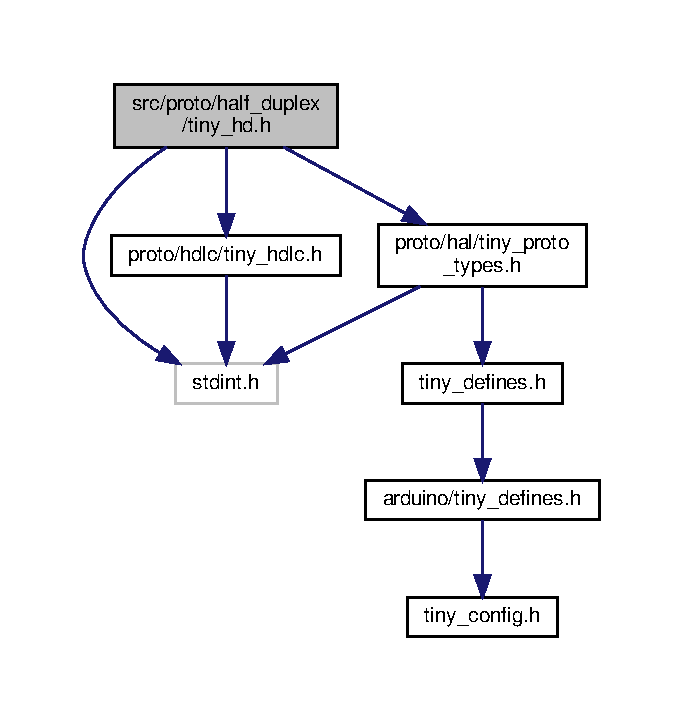
\includegraphics[width=332pt]{tiny__hd_8h__incl}
\end{center}
\end{figure}
This graph shows which files directly or indirectly include this file\+:\nopagebreak
\begin{figure}[H]
\begin{center}
\leavevmode
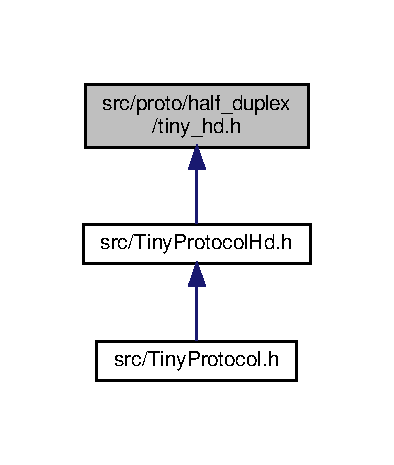
\includegraphics[width=199pt]{tiny__hd_8h__dep__incl}
\end{center}
\end{figure}
\subsection*{Classes}
\begin{DoxyCompactItemize}
\item 
struct \hyperlink{structSTinyHdData__}{S\+Tiny\+Hd\+Data\+\_\+}
\item 
struct \hyperlink{structSTinyHdInit__}{S\+Tiny\+Hd\+Init\+\_\+}
\end{DoxyCompactItemize}
\subsection*{Typedefs}
\begin{DoxyCompactItemize}
\item 
typedef struct \hyperlink{structSTinyHdData__}{S\+Tiny\+Hd\+Data\+\_\+} \hyperlink{group__HALF__DUPLEX__API_gaf9f81ad129b754a780dfca5dcd7f7cf9}{S\+Tiny\+Hd\+Data}
\item 
typedef struct \hyperlink{structSTinyHdInit__}{S\+Tiny\+Hd\+Init\+\_\+} \hyperlink{group__HALF__DUPLEX__API_ga784f1a0f0ae7f06da4bc288fa3f22408}{S\+Tiny\+Hd\+Init}
\end{DoxyCompactItemize}
\subsection*{Functions}
\begin{DoxyCompactItemize}
\item 
int \hyperlink{group__HALF__DUPLEX__API_ga747e6a3a0b5d2a9e1fe0c143c20057e9}{tiny\+\_\+hd\+\_\+init} (\hyperlink{group__HALF__DUPLEX__API_gaf9f81ad129b754a780dfca5dcd7f7cf9}{S\+Tiny\+Hd\+Data} $\ast$handle, \hyperlink{group__HALF__DUPLEX__API_ga784f1a0f0ae7f06da4bc288fa3f22408}{S\+Tiny\+Hd\+Init} $\ast$init)
\begin{DoxyCompactList}\small\item\em Initialized communication for Tiny Half Duplex protocol. \end{DoxyCompactList}\item 
void \hyperlink{group__HALF__DUPLEX__API_ga275846730a88b9654345d5defbda31e7}{tiny\+\_\+hd\+\_\+close} (\hyperlink{group__HALF__DUPLEX__API_gaf9f81ad129b754a780dfca5dcd7f7cf9}{S\+Tiny\+Hd\+Data} $\ast$handle)
\begin{DoxyCompactList}\small\item\em stops Tiny Half Duplex state machine \end{DoxyCompactList}\item 
int \hyperlink{group__HALF__DUPLEX__API_gac962595f09883dea1dd0992a608a17b9}{tiny\+\_\+hd\+\_\+run} (\hyperlink{group__HALF__DUPLEX__API_gaf9f81ad129b754a780dfca5dcd7f7cf9}{S\+Tiny\+Hd\+Data} $\ast$handle)
\begin{DoxyCompactList}\small\item\em runs receive functions of Tiny Half Duplex protocol. \end{DoxyCompactList}\item 
int \hyperlink{group__HALF__DUPLEX__API_ga84325cc961c3f31e2ba6111d0235bd61}{tiny\+\_\+hd\+\_\+run\+\_\+tx} (\hyperlink{group__HALF__DUPLEX__API_gaf9f81ad129b754a780dfca5dcd7f7cf9}{S\+Tiny\+Hd\+Data} $\ast$handle)
\item 
int \hyperlink{group__HALF__DUPLEX__API_ga5aad8dcb504b80bac923496f2686a6d6}{tiny\+\_\+send\+\_\+wait\+\_\+ack} (\hyperlink{group__HALF__DUPLEX__API_gaf9f81ad129b754a780dfca5dcd7f7cf9}{S\+Tiny\+Hd\+Data} $\ast$handle, void $\ast$buf, uint16\+\_\+t len)
\begin{DoxyCompactList}\small\item\em Sends userdata and waits for acknowledgement from remote side. \end{DoxyCompactList}\end{DoxyCompactItemize}


\subsection{Detailed Description}
Tiny Protocol Half Duplex A\+PI. 

This is Tiny Half-\/\+Duplex protocol implementation for microcontrollers. It is built on top of Tiny Protocol (tiny\+\_\+layer2.\+c) 
\hypertarget{tiny__light_8h}{}\section{src/proto/light/tiny\+\_\+light.h File Reference}
\label{tiny__light_8h}\index{src/proto/light/tiny\+\_\+light.\+h@{src/proto/light/tiny\+\_\+light.\+h}}


Tiny Light protocol A\+PI.  


{\ttfamily \#include \char`\"{}proto/hdlc/tiny\+\_\+hdlc.\+h\char`\"{}}\newline
{\ttfamily \#include \char`\"{}proto/hal/tiny\+\_\+types.\+h\char`\"{}}\newline
Include dependency graph for tiny\+\_\+light.\+h\+:
\nopagebreak
\begin{figure}[H]
\begin{center}
\leavevmode
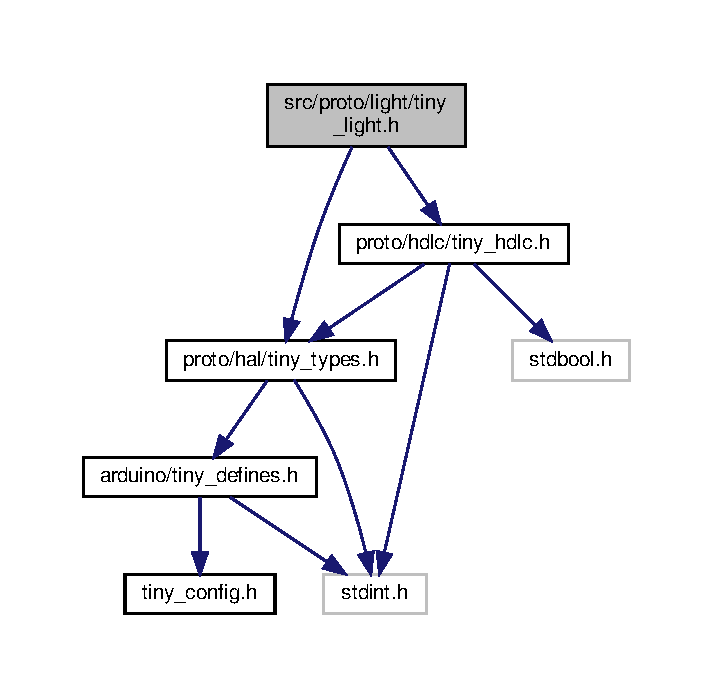
\includegraphics[width=342pt]{tiny__light_8h__incl}
\end{center}
\end{figure}
This graph shows which files directly or indirectly include this file\+:
\nopagebreak
\begin{figure}[H]
\begin{center}
\leavevmode
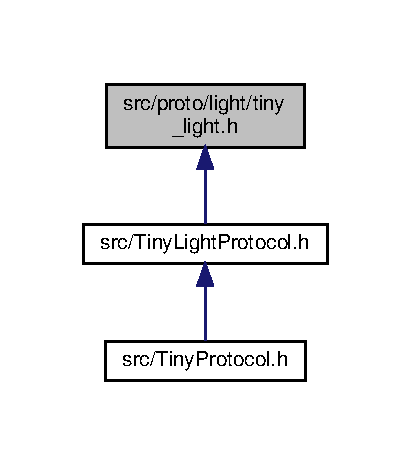
\includegraphics[width=197pt]{tiny__light_8h__dep__incl}
\end{center}
\end{figure}
\subsection*{Classes}
\begin{DoxyCompactItemize}
\item 
struct \hyperlink{structSTinyLightData}{S\+Tiny\+Light\+Data}
\end{DoxyCompactItemize}
\subsection*{Functions}
\begin{DoxyCompactItemize}
\item 
int \hyperlink{group__LIGHT__API_ga221cf790724163d1aee89ad6a6c9a14d}{tiny\+\_\+light\+\_\+init} (void $\ast$handle, \hyperlink{tiny__types_8h_aafd634660bba76cace57a8f9b01e044d}{write\+\_\+block\+\_\+cb\+\_\+t} write\+\_\+func, \hyperlink{tiny__types_8h_a15bec127d9ee63658563d62e92b5261b}{read\+\_\+block\+\_\+cb\+\_\+t} read\+\_\+func, void $\ast$pdata)
\item 
int \hyperlink{group__LIGHT__API_ga6e045b8f4ef551c274fbacaa625e2748}{tiny\+\_\+light\+\_\+close} (void $\ast$handle)
\item 
int \hyperlink{group__LIGHT__API_ga12391f0d4c06fb6296b84fd4681a87f7}{tiny\+\_\+light\+\_\+send} (void $\ast$handle, const uint8\+\_\+t $\ast$pbuf, int len)
\begin{DoxyCompactList}\small\item\em sends frame with user payload to communication channel in blocking mode \end{DoxyCompactList}\item 
int \hyperlink{group__LIGHT__API_ga0181db79922917957779e1f2d740c407}{tiny\+\_\+light\+\_\+read} (void $\ast$handle, uint8\+\_\+t $\ast$pbuf, int len)
\begin{DoxyCompactList}\small\item\em reads frame from the channel in blocking mode. \end{DoxyCompactList}\item 
\hyperlink{struct__hdlc__handle__t}{hdlc\+\_\+handle\+\_\+t} \hyperlink{group__LIGHT__API_gabf582877977ecd57299d8675a1279e36}{tiny\+\_\+light\+\_\+get\+\_\+hdlc} (void $\ast$handle)
\begin{DoxyCompactList}\small\item\em returns lower level hdlc handle. \end{DoxyCompactList}\end{DoxyCompactItemize}


\subsection{Detailed Description}
Tiny Light protocol A\+PI. 

This is Tiny Light protocol implementation for microcontrollers 
\hypertarget{TinyLightProtocol_8h}{}\section{src/\+Tiny\+Light\+Protocol.h File Reference}
\label{TinyLightProtocol_8h}\index{src/\+Tiny\+Light\+Protocol.\+h@{src/\+Tiny\+Light\+Protocol.\+h}}


Tiny light protocol Arduino A\+PI.  


{\ttfamily \#include \char`\"{}Tiny\+Packet.\+h\char`\"{}}\newline
{\ttfamily \#include \char`\"{}proto/tiny\+\_\+light.\+h\char`\"{}}\newline
{\ttfamily \#include $<$Hardware\+Serial.\+h$>$}\newline
Include dependency graph for Tiny\+Light\+Protocol.\+h\+:
\nopagebreak
\begin{figure}[H]
\begin{center}
\leavevmode
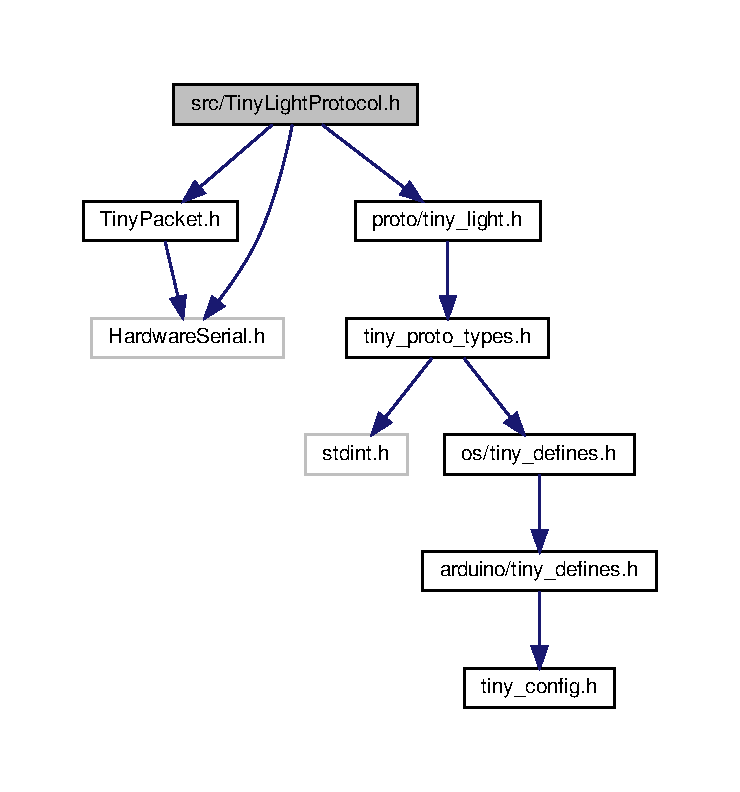
\includegraphics[width=350pt]{TinyLightProtocol_8h__incl}
\end{center}
\end{figure}
\subsection*{Classes}
\begin{DoxyCompactItemize}
\item 
class \hyperlink{classTiny_1_1ProtoLight}{Tiny\+::\+Proto\+Light}
\end{DoxyCompactItemize}


\subsection{Detailed Description}
Tiny light protocol Arduino A\+PI. 

This is Tiny light protocol implementation for microcontrollers 
\hypertarget{TinyPacket_8h}{}\section{src/\+Tiny\+Packet.h File Reference}
\label{TinyPacket_8h}\index{src/\+Tiny\+Packet.\+h@{src/\+Tiny\+Packet.\+h}}


Tiny protocol Arduino A\+PI.  


{\ttfamily \#include $<$Hardware\+Serial.\+h$>$}\newline
Include dependency graph for Tiny\+Packet.\+h\+:\nopagebreak
\begin{figure}[H]
\begin{center}
\leavevmode
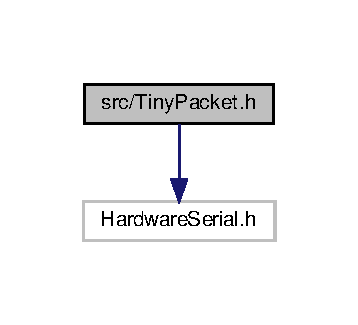
\includegraphics[width=172pt]{TinyPacket_8h__incl}
\end{center}
\end{figure}
This graph shows which files directly or indirectly include this file\+:\nopagebreak
\begin{figure}[H]
\begin{center}
\leavevmode
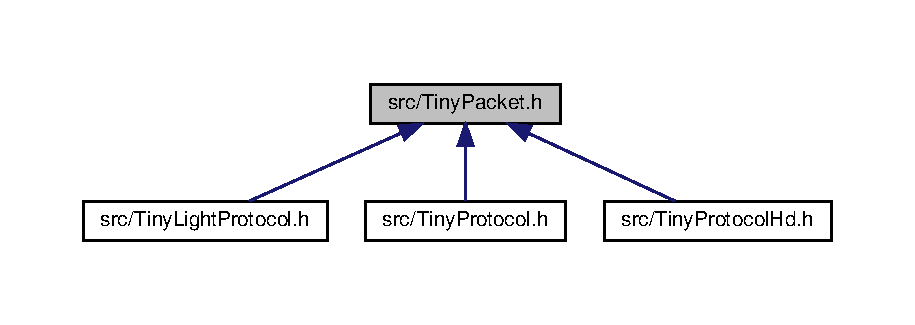
\includegraphics[width=350pt]{TinyPacket_8h__dep__incl}
\end{center}
\end{figure}
\subsection*{Classes}
\begin{DoxyCompactItemize}
\item 
class \hyperlink{classTiny_1_1Packet}{Tiny\+::\+Packet}
\end{DoxyCompactItemize}


\subsection{Detailed Description}
Tiny protocol Arduino A\+PI. 

This is Tiny protocol implementation for microcontrollers 
\hypertarget{TinyProtocol_8h}{}\section{src/arduino/src/\+Tiny\+Protocol.h File Reference}
\label{TinyProtocol_8h}\index{src/arduino/src/\+Tiny\+Protocol.\+h@{src/arduino/src/\+Tiny\+Protocol.\+h}}


Tiny protocol Arduino A\+P\+I.  


{\ttfamily \#include \char`\"{}proto/tiny\+\_\+layer2.\+h\char`\"{}}\\*
{\ttfamily \#include $<$Hardware\+Serial.\+h$>$}\\*
Include dependency graph for Tiny\+Protocol.\+h\+:
\nopagebreak
\begin{figure}[H]
\begin{center}
\leavevmode
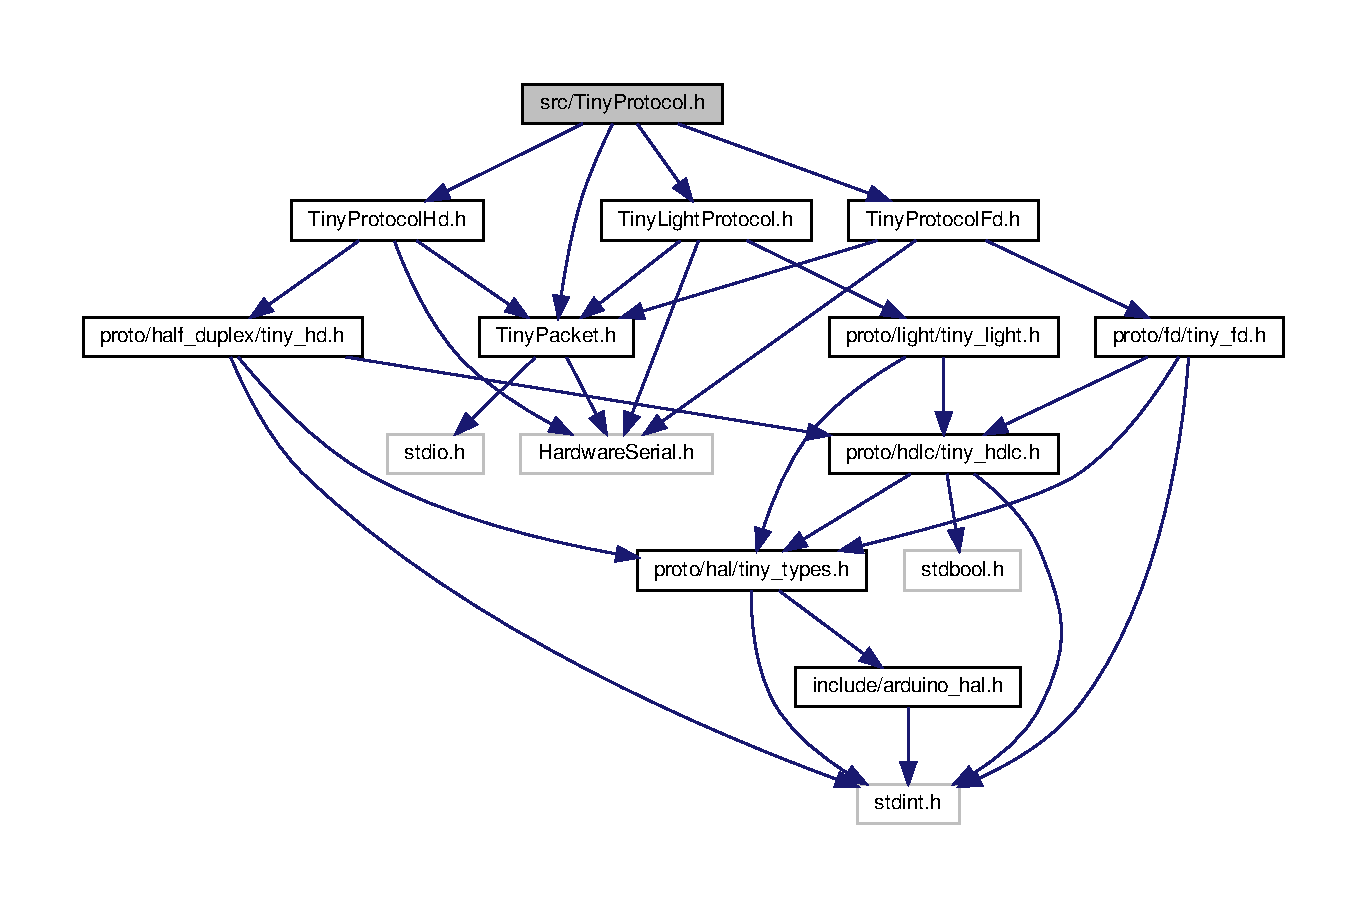
\includegraphics[width=350pt]{TinyProtocol_8h__incl}
\end{center}
\end{figure}
\subsection*{Classes}
\begin{DoxyCompactItemize}
\item 
class \hyperlink{classTiny_1_1Proto}{Tiny\+::\+Proto}
\item 
class \hyperlink{classTiny_1_1Packet}{Tiny\+::\+Packet}
\end{DoxyCompactItemize}


\subsection{Detailed Description}
Tiny protocol Arduino A\+P\+I. 

This is Tiny protocol implementation for microcontrollers 
\hypertarget{TinyProtocolFd_8h}{}\section{src/\+Tiny\+Protocol\+Fd.h File Reference}
\label{TinyProtocolFd_8h}\index{src/\+Tiny\+Protocol\+Fd.\+h@{src/\+Tiny\+Protocol\+Fd.\+h}}


Tiny protocol Arduino A\+PI.  


{\ttfamily \#include \char`\"{}Tiny\+Packet.\+h\char`\"{}}\newline
{\ttfamily \#include \char`\"{}proto/fd/tiny\+\_\+fd.\+h\char`\"{}}\newline
{\ttfamily \#include $<$Hardware\+Serial.\+h$>$}\newline
Include dependency graph for Tiny\+Protocol\+Fd.\+h\+:
\nopagebreak
\begin{figure}[H]
\begin{center}
\leavevmode
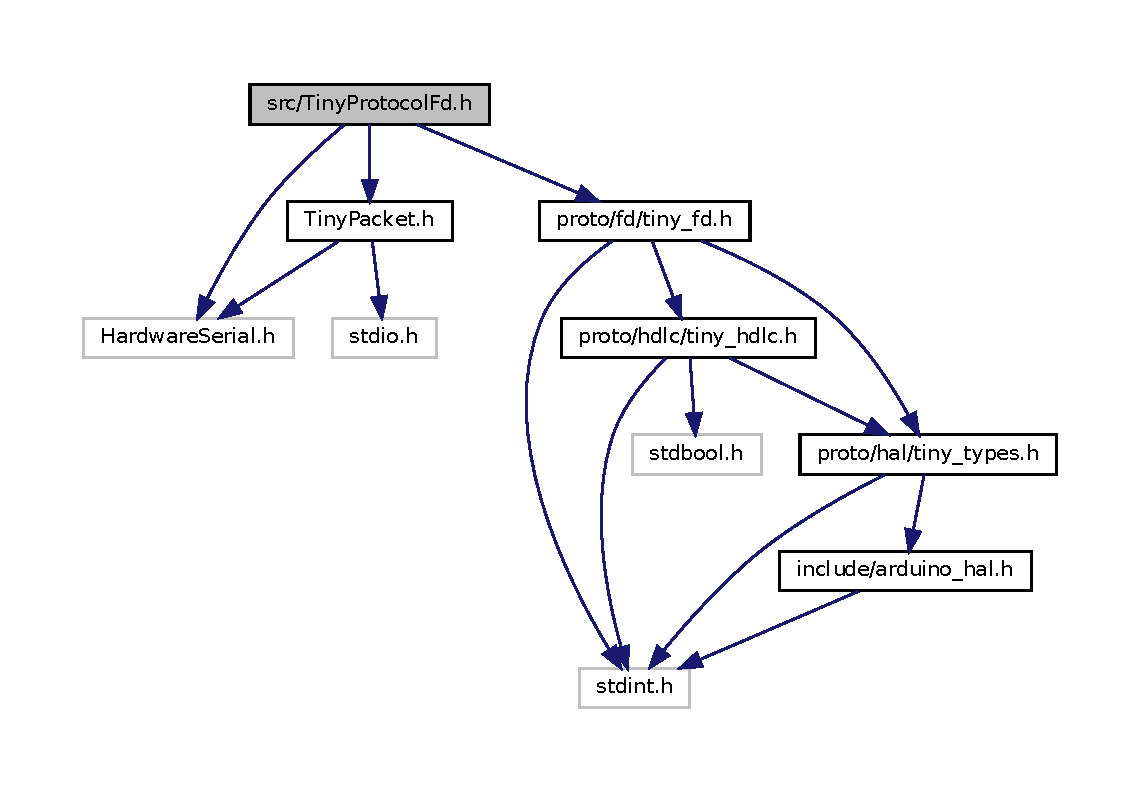
\includegraphics[width=350pt]{TinyProtocolFd_8h__incl}
\end{center}
\end{figure}
This graph shows which files directly or indirectly include this file\+:
\nopagebreak
\begin{figure}[H]
\begin{center}
\leavevmode
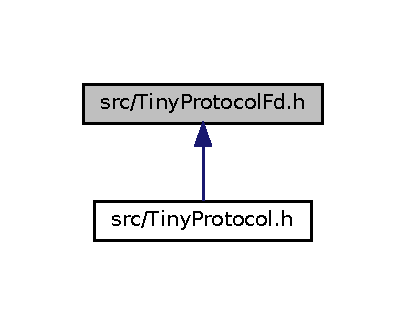
\includegraphics[width=195pt]{TinyProtocolFd_8h__dep__incl}
\end{center}
\end{figure}
\subsection*{Classes}
\begin{DoxyCompactItemize}
\item 
class \hyperlink{classTiny_1_1IProtoFd}{Tiny\+::\+I\+Proto\+Fd}
\item 
class \hyperlink{classTiny_1_1ProtoFd}{Tiny\+::\+Proto\+Fd$<$ S $>$}
\item 
class \hyperlink{classTiny_1_1ProtoFdD}{Tiny\+::\+Proto\+FdD}
\end{DoxyCompactItemize}


\subsection{Detailed Description}
Tiny protocol Arduino A\+PI. 

This is Tiny protocol implementation for microcontrollers 
\hypertarget{TinyProtocolHd_8h}{}\section{src/arduino/src/\+Tiny\+Protocol\+Hd.h File Reference}
\label{TinyProtocolHd_8h}\index{src/arduino/src/\+Tiny\+Protocol\+Hd.\+h@{src/arduino/src/\+Tiny\+Protocol\+Hd.\+h}}


Tiny protocol Arduino A\+P\+I.  


{\ttfamily \#include \char`\"{}Tiny\+Packet.\+h\char`\"{}}\\*
{\ttfamily \#include \char`\"{}proto/tiny\+\_\+hd.\+h\char`\"{}}\\*
{\ttfamily \#include $<$Hardware\+Serial.\+h$>$}\\*
Include dependency graph for Tiny\+Protocol\+Hd.\+h\+:
\nopagebreak
\begin{figure}[H]
\begin{center}
\leavevmode
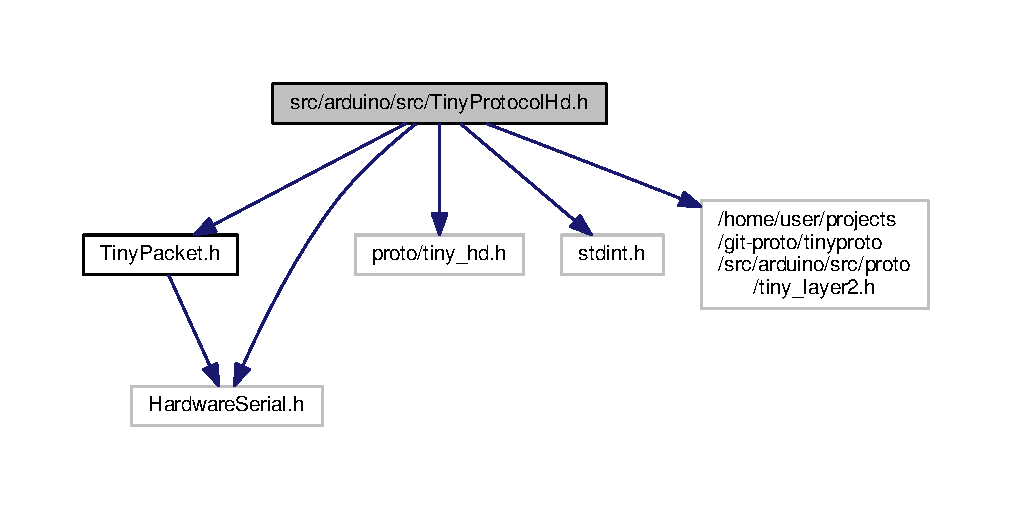
\includegraphics[width=350pt]{TinyProtocolHd_8h__incl}
\end{center}
\end{figure}
\subsection*{Classes}
\begin{DoxyCompactItemize}
\item 
class \hyperlink{classTiny_1_1ProtoHd}{Tiny\+::\+Proto\+Hd}
\end{DoxyCompactItemize}


\subsection{Detailed Description}
Tiny protocol Arduino A\+P\+I. 

This is Tiny protocol implementation for microcontrollers 
%--- End generated contents ---

% Index
\backmatter
\newpage
\phantomsection
\clearemptydoublepage
\addcontentsline{toc}{chapter}{Index}
\printindex

\end{document}
